В качестве исходного сигнала рассмотрим функцию

\begin{equation}
    g(t)=\begin{cases}
        3, & t \in [-2, 5] \\
        0, & t \in (-\infty,2)\cup (5,\infty)

    \end{cases},
\end{equation}

график которой приведен ниже:

\begin{figure}[ht!]
    \centering
    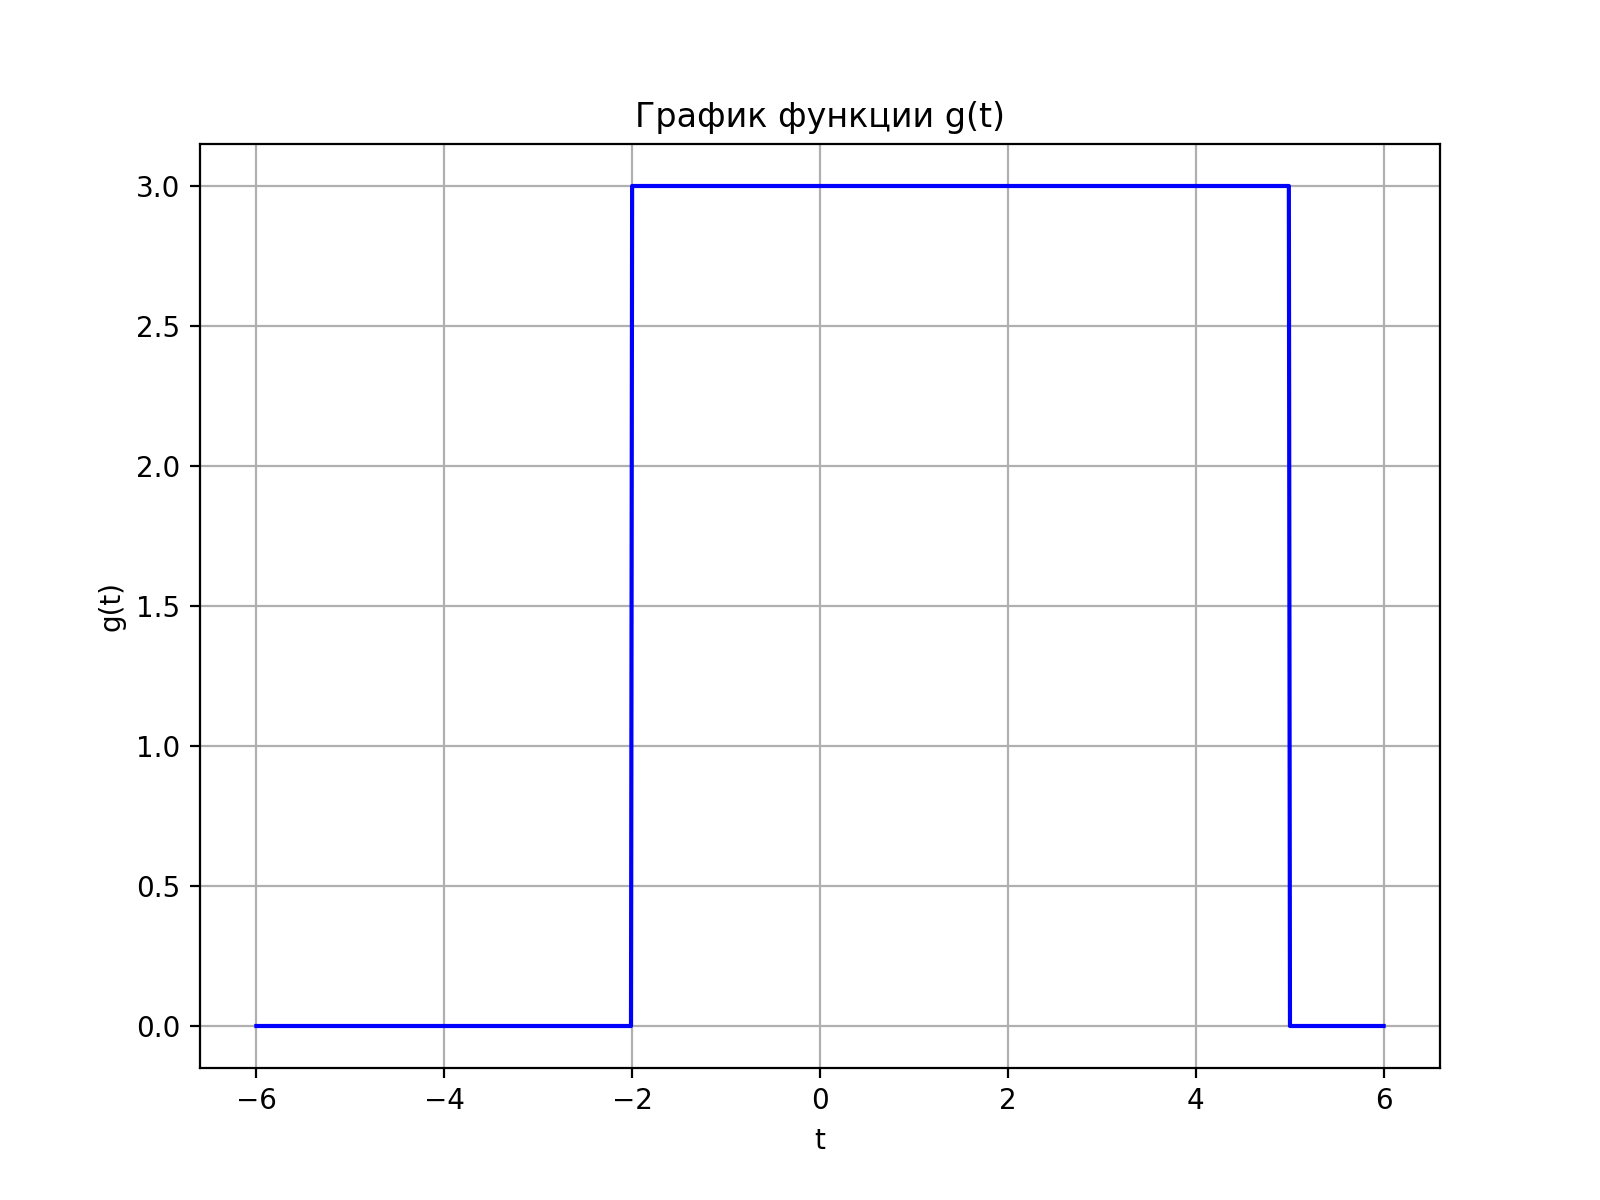
\includegraphics[width=\textwidth]{media/1 task/high_freq/Initial.png}
    \caption{График функции $g(t)$}
    \label{fig:initial}
\end{figure}

\clearpage

Для выполнения первого задания нам необходимо создать зашумлённую версию функции, или сигнала, при помощи функции

\begin{equation}
    u(t)=g(t)+b(rand(size(t))-0.5)+c*\sin(d*t),
\end{equation}

в которой $b$, $c$, $d$ - параметры, чьё влияние на фильтрацию сигнала $u(t)$ мы будем исследовать в этом задании.

\subsection{Высокие частоты}\label{high_freq}

При выполнении этого пункта значение параметра $c$ мы примем равным $0$. Параметр $b$ принимает значения $0.25, 1, 4$. Графики зашумлённого сигнала приведены ниже:

\begin{figure}[ht!]
    \centering
    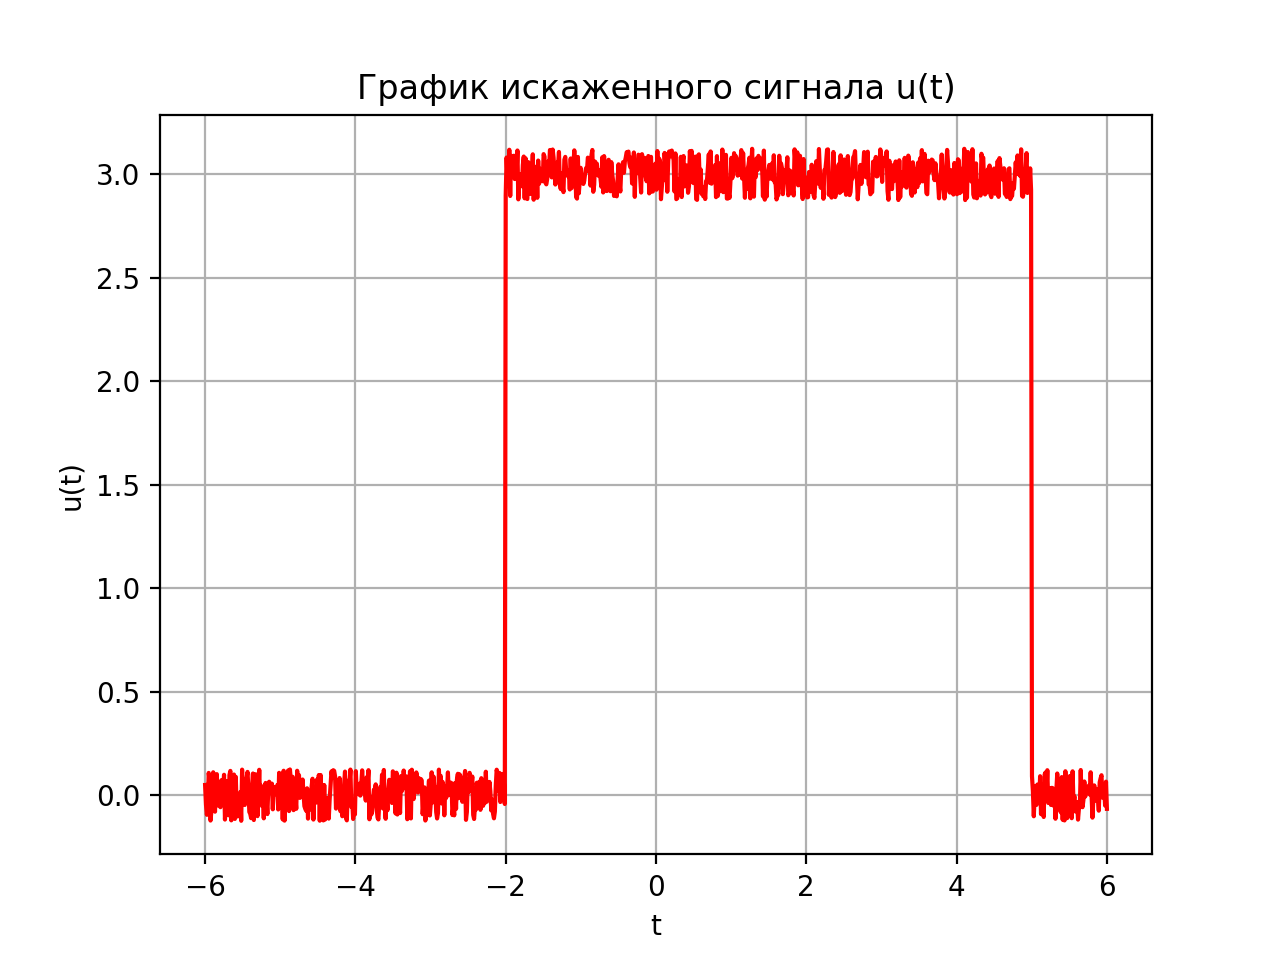
\includegraphics[scale=0.75]{media/1 task/high_freq/Noisy_0,25.png}
    \caption{График функции $u(t)$ при $b=0.25$}
    \label{fig:noisy_025}
\end{figure}

\clearpage

\begin{figure}[ht!]
    \centering
    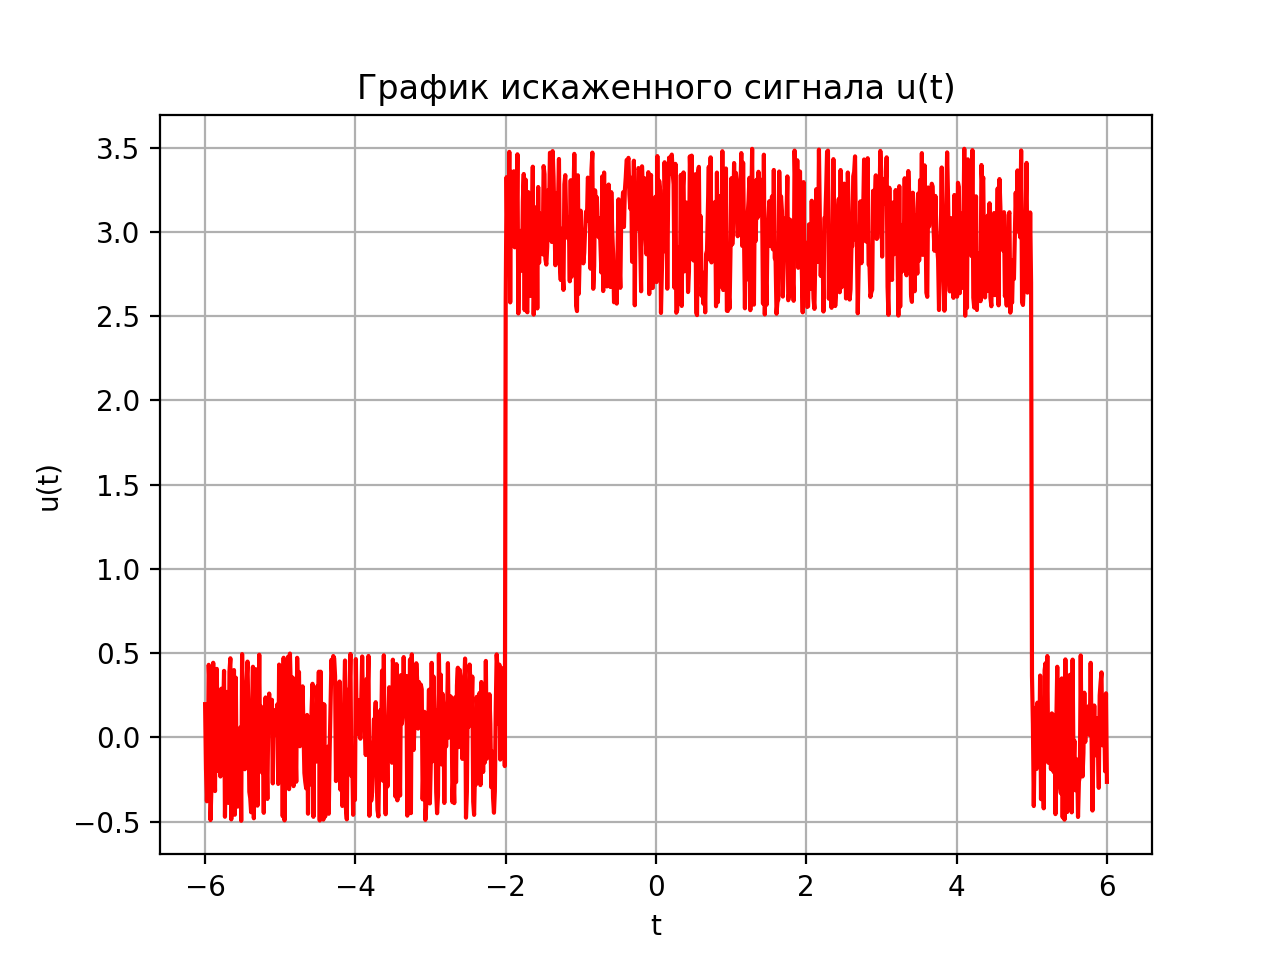
\includegraphics[scale=0.75]{media/1 task/high_freq/Noisy_1.png}
    \caption{График функции $u(t)$ при $b=1$}
    \label{fig:noisy_1}
\end{figure}

\begin{figure}[ht!]
    \centering
    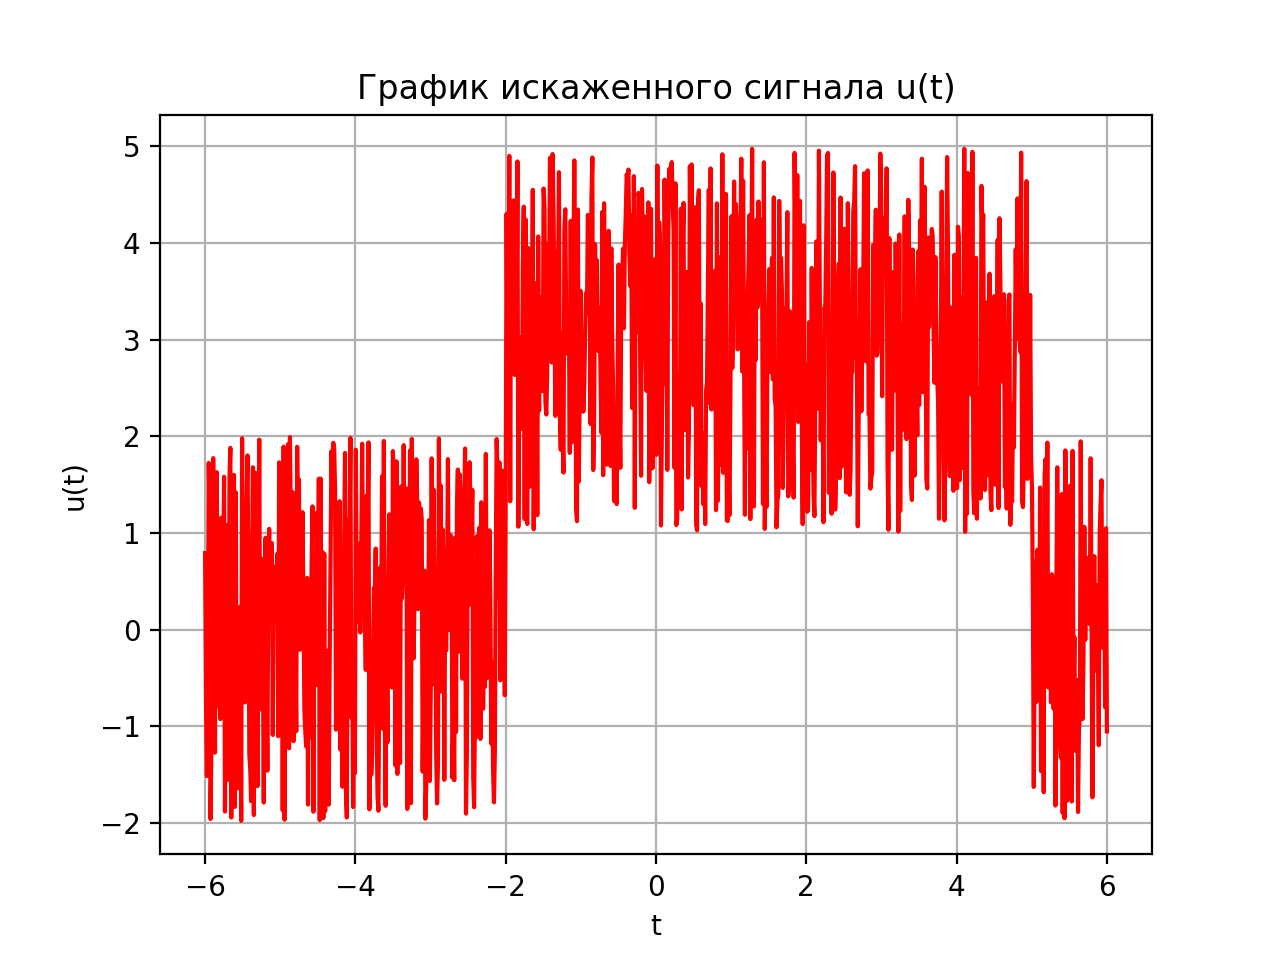
\includegraphics[scale=0.75]{media/1 task/high_freq/Noisy_4.png}
    \caption{График функции $u(t)$ при $b=4$}
    \label{fig:noisy_4}
\end{figure}

Благодаря графикам мы можем сделать вывод о том, что параметр $b$ влияет на степень хаотического шума, точнее на его амплитуду. Переходим к фильтрации!
\subsubsection{Режем Фурье-образы и фильтруем сигнал!}
 
Снова обращаемся к замечательному Фурье-преобразованию! Для выполнения задания 1 будем выполнять его для частоты $\nu$. В качестве частот среза ($\nu_0$) будут выступать значения $0.6, 1.2, 1.8$ Гц. Построим графики модулей Фурье-образов сигнала $u(t)$ и отфильтрованного сигнала, а также сравнительные графики модулей $g(t)$ и отфильтрованного сигнала:

\begin{figure}[ht!]
    \centering
    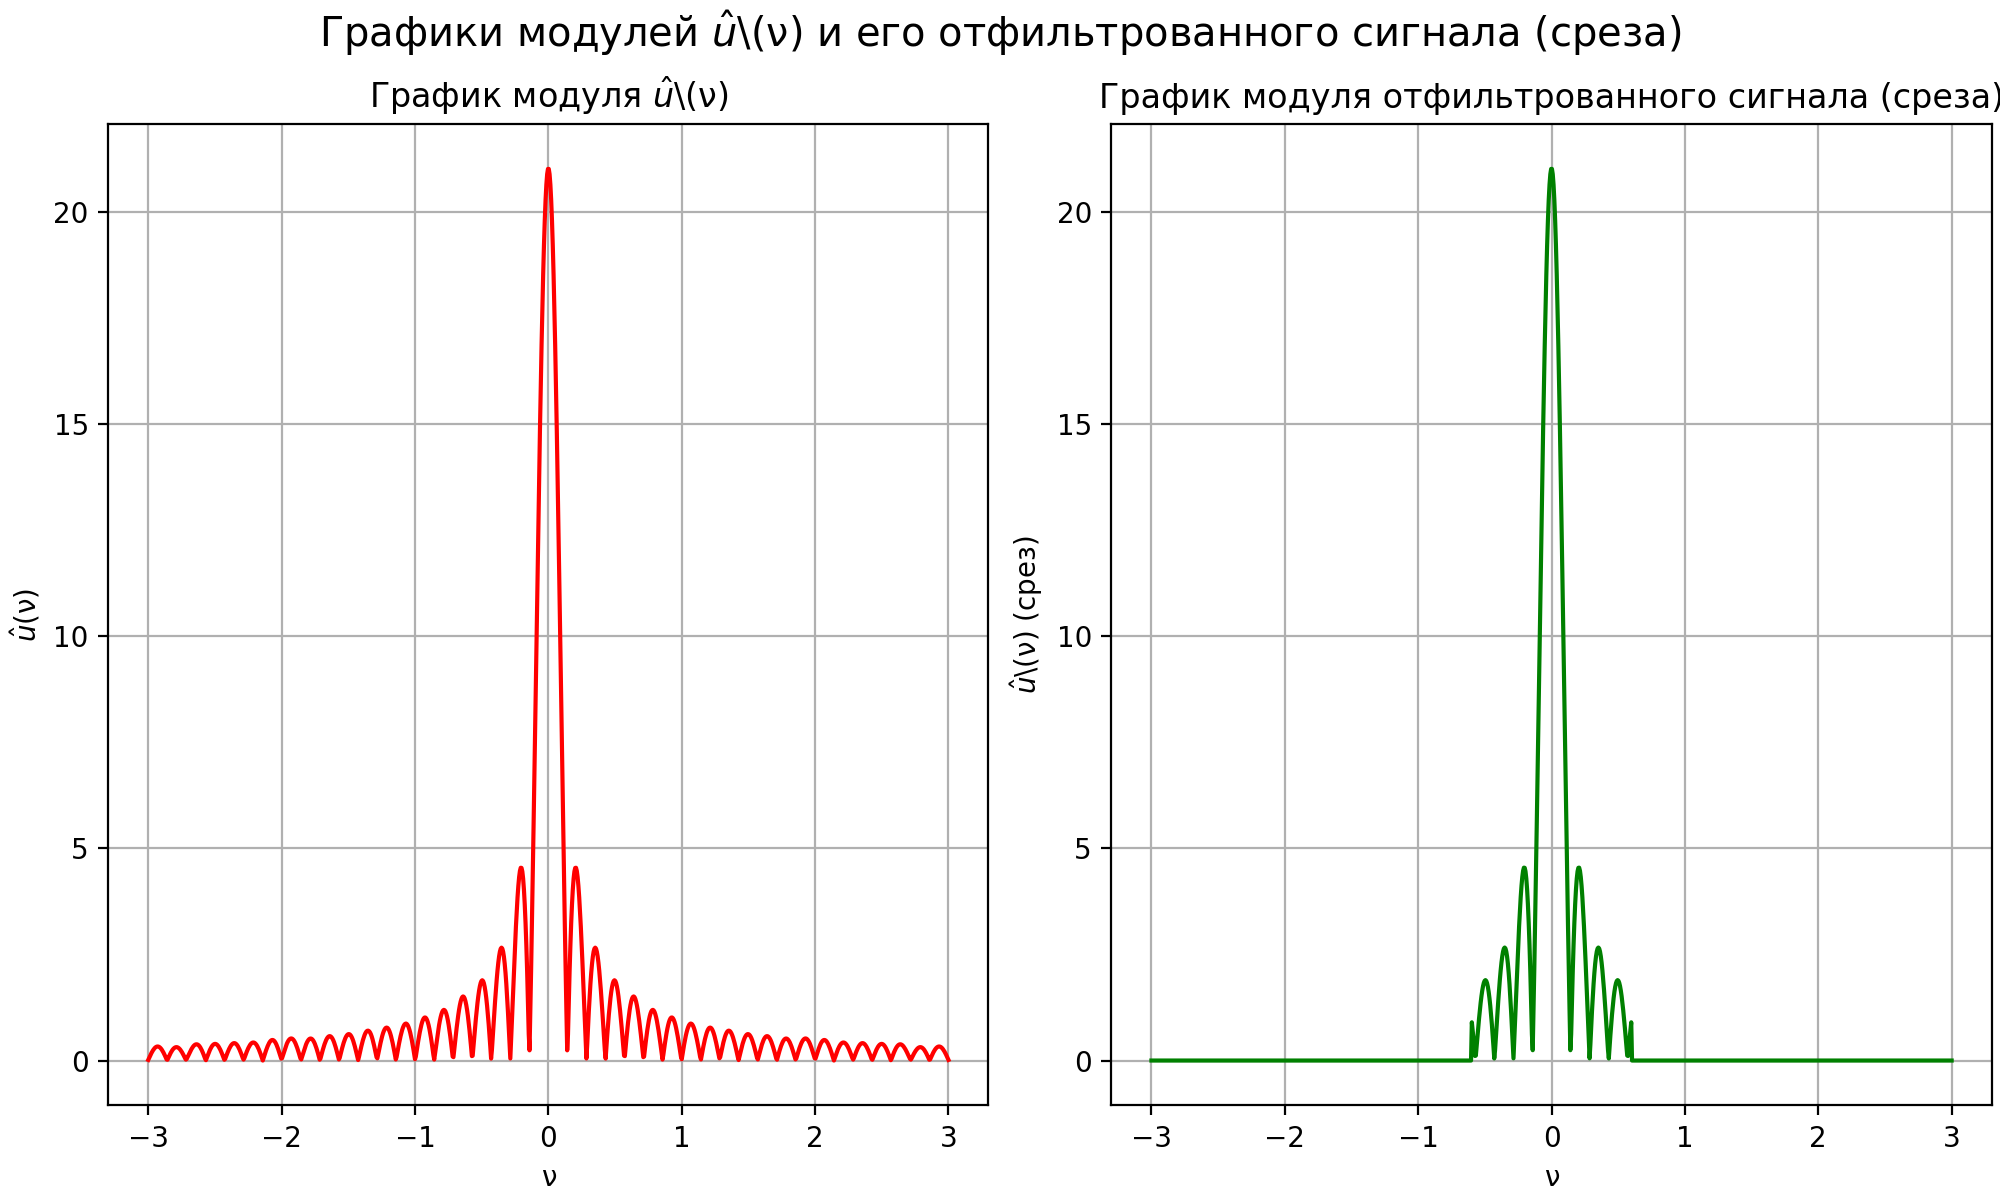
\includegraphics[scale=0.55]{media/1 task/high_freq/Fourier_Image_0,25_-0,5975975975975976.png}
    \caption{Графики модулей Фурье-образа $u(t)$ и отфильтрованного сигнала при $b=0.25$ и $\nu_0=0.6$ Гц}
    \label{fig:four_025_06}
\end{figure}

\begin{figure}[ht!]
    \centering
    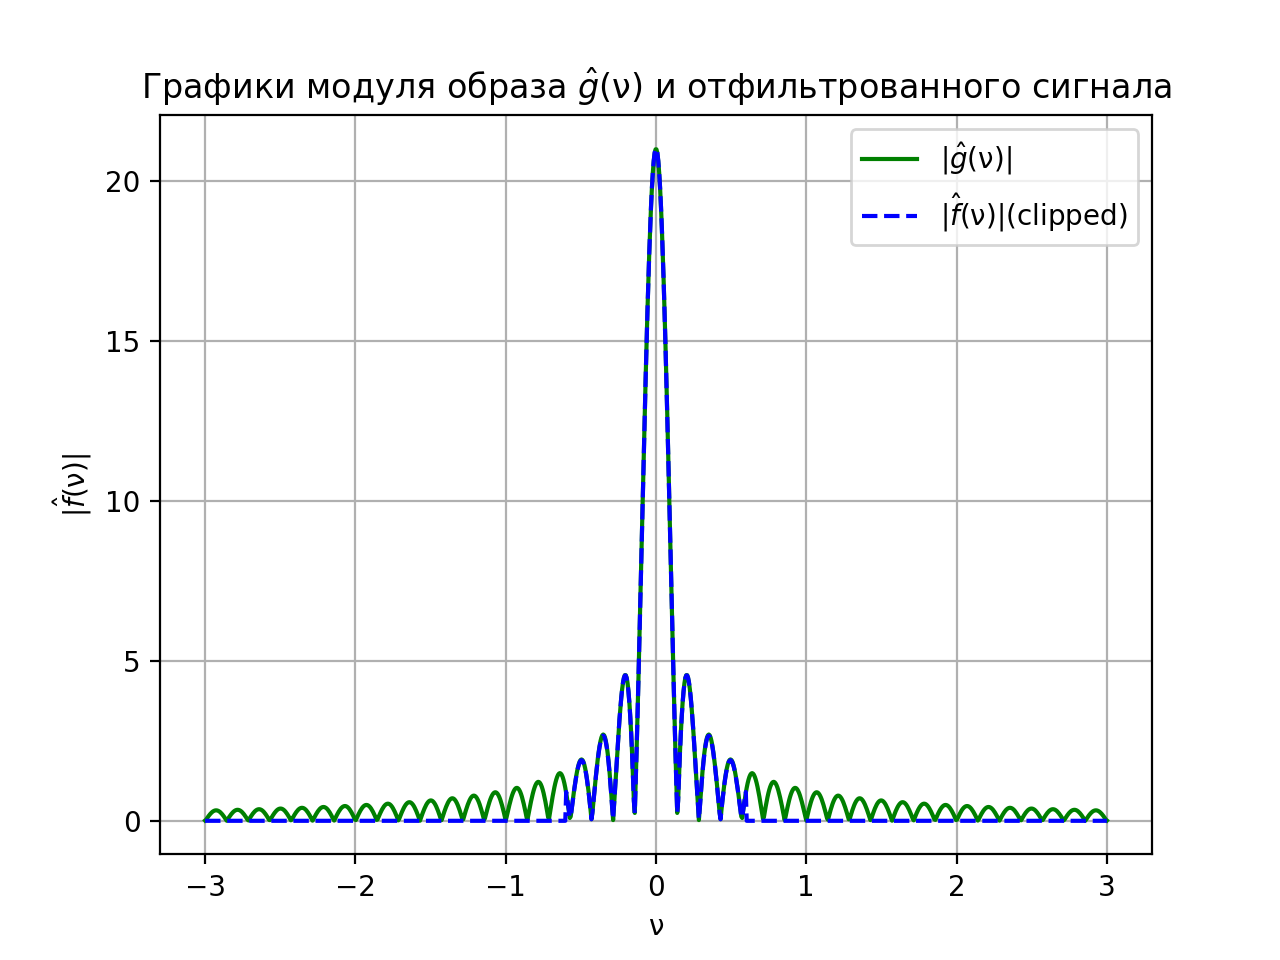
\includegraphics[scale=0.55]{media/1 task/high_freq/Fourier_Image_Comparison_0,25_-0,5975975975975976.png}
    \caption{Сравнительные графики модулей Фурье-образа $g(t)$ и отфильтрованного сигнала при $b=0.25$ и $\nu_0=0.6$ Гц}
    \label{fig:fourc_025_06}
\end{figure}

\begin{figure}[ht!]
    \centering
    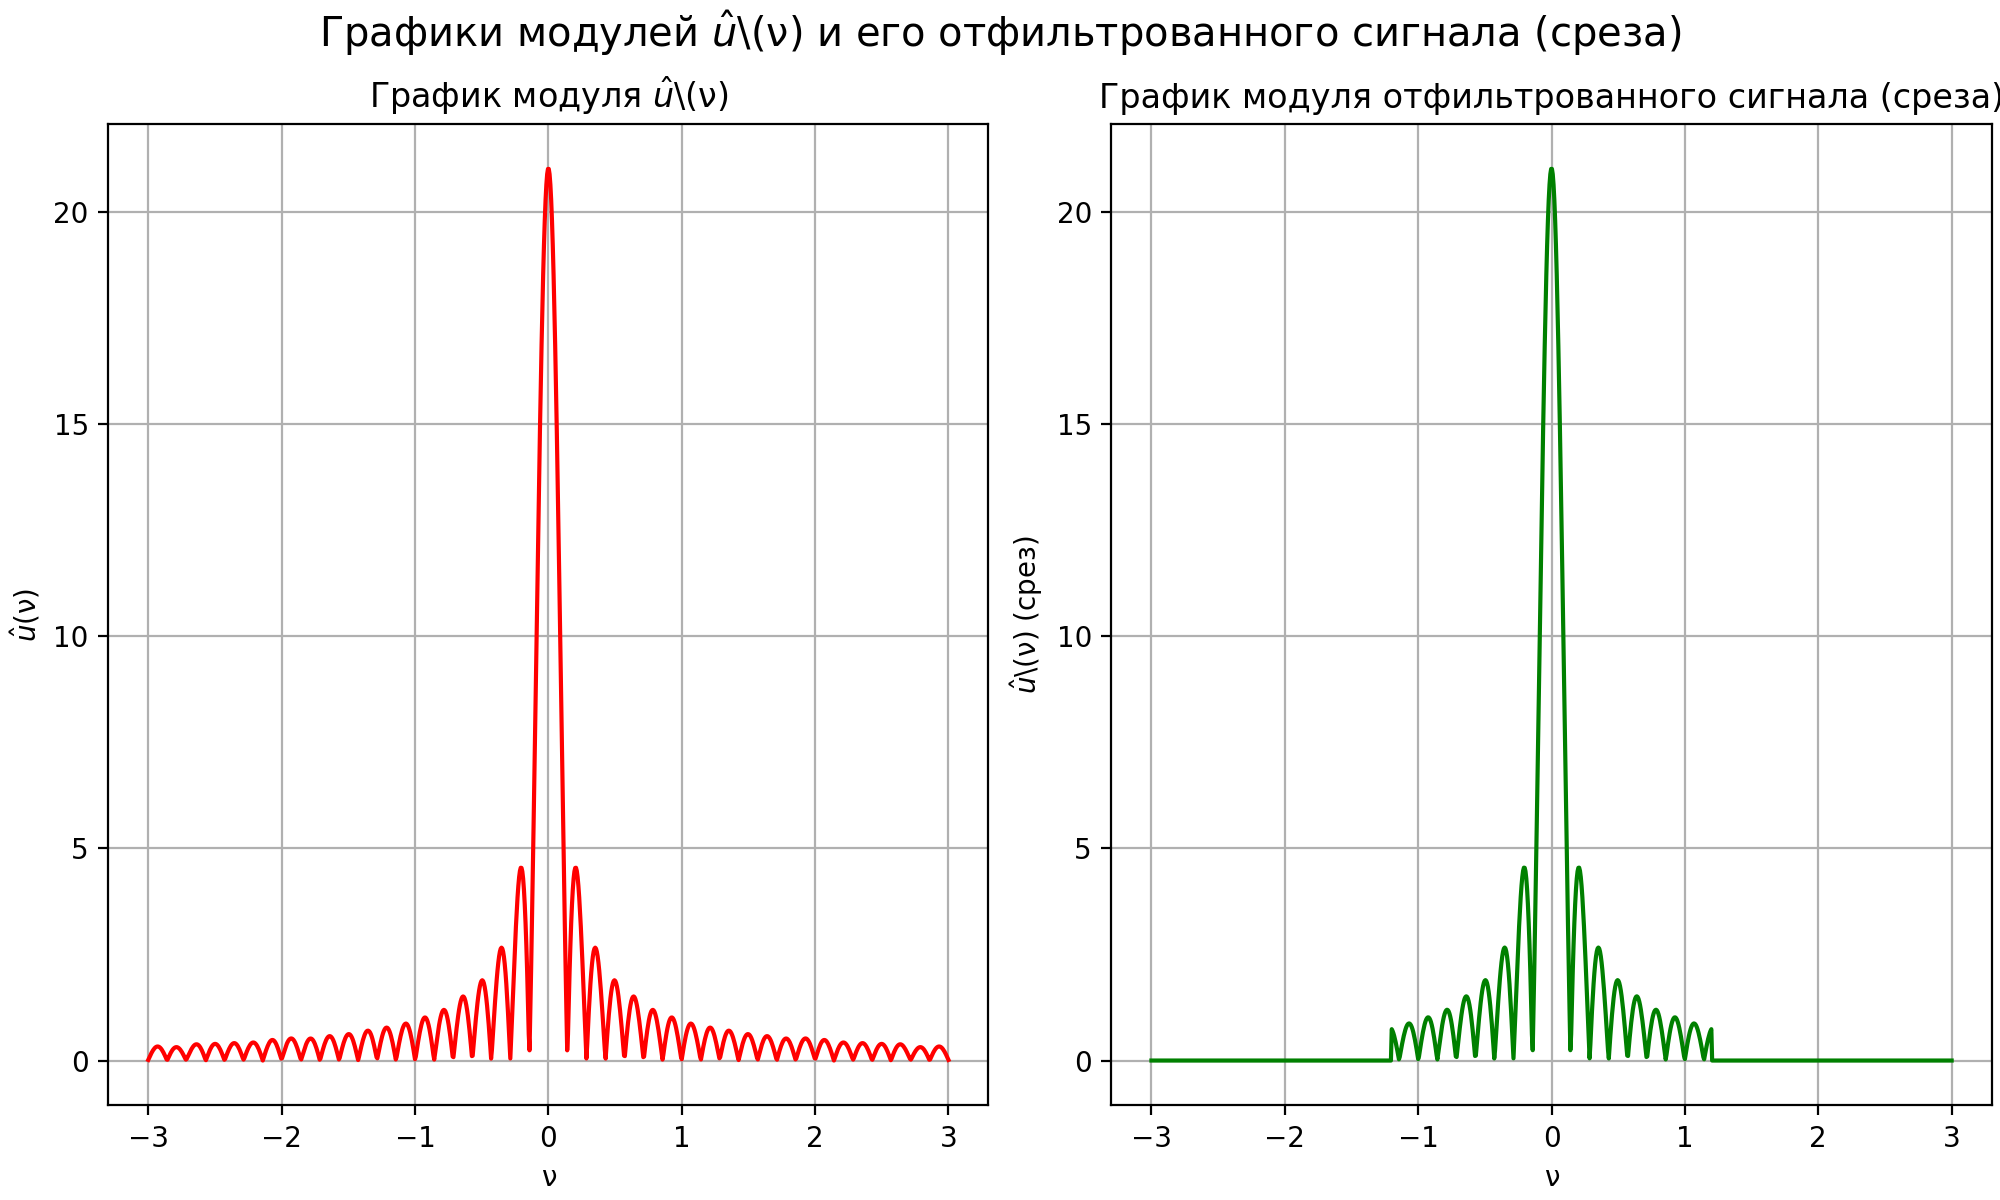
\includegraphics[scale=0.55]{media/1 task/high_freq/Fourier_Image_0,25_-1,1981981981981982.png}
    \caption{Графики модулей Фурье-образа $u(t)$ и отфильтрованного сигнала при $b=0.25$ и $\nu_0=1.2$ Гц}
    \label{fig:four_025_12}
\end{figure}

\begin{figure}[ht!]
    \centering
    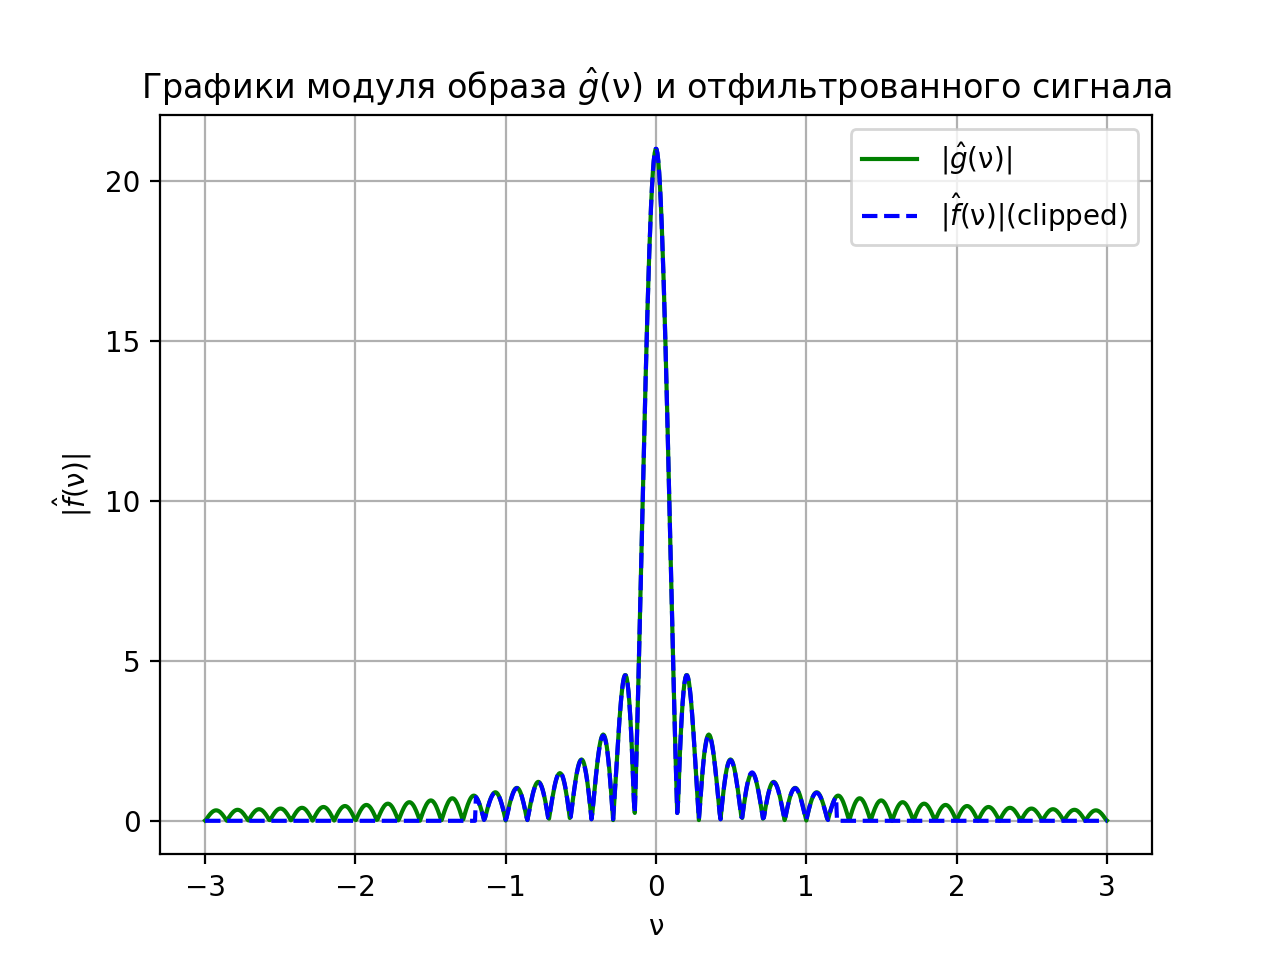
\includegraphics[scale=0.55]{media/1 task/high_freq/Fourier_Image_Comparison_0,25_-1,1981981981981982.png}
    \caption{Сравнительные графики модулей Фурье-образа $g(t)$ и отфильтрованного сигнала при $b=0.25$ и $\nu_0=1.2$ Гц}
    \label{fig:fourc_025_12}
\end{figure}

\clearpage

\begin{figure}[ht!]
    \centering
    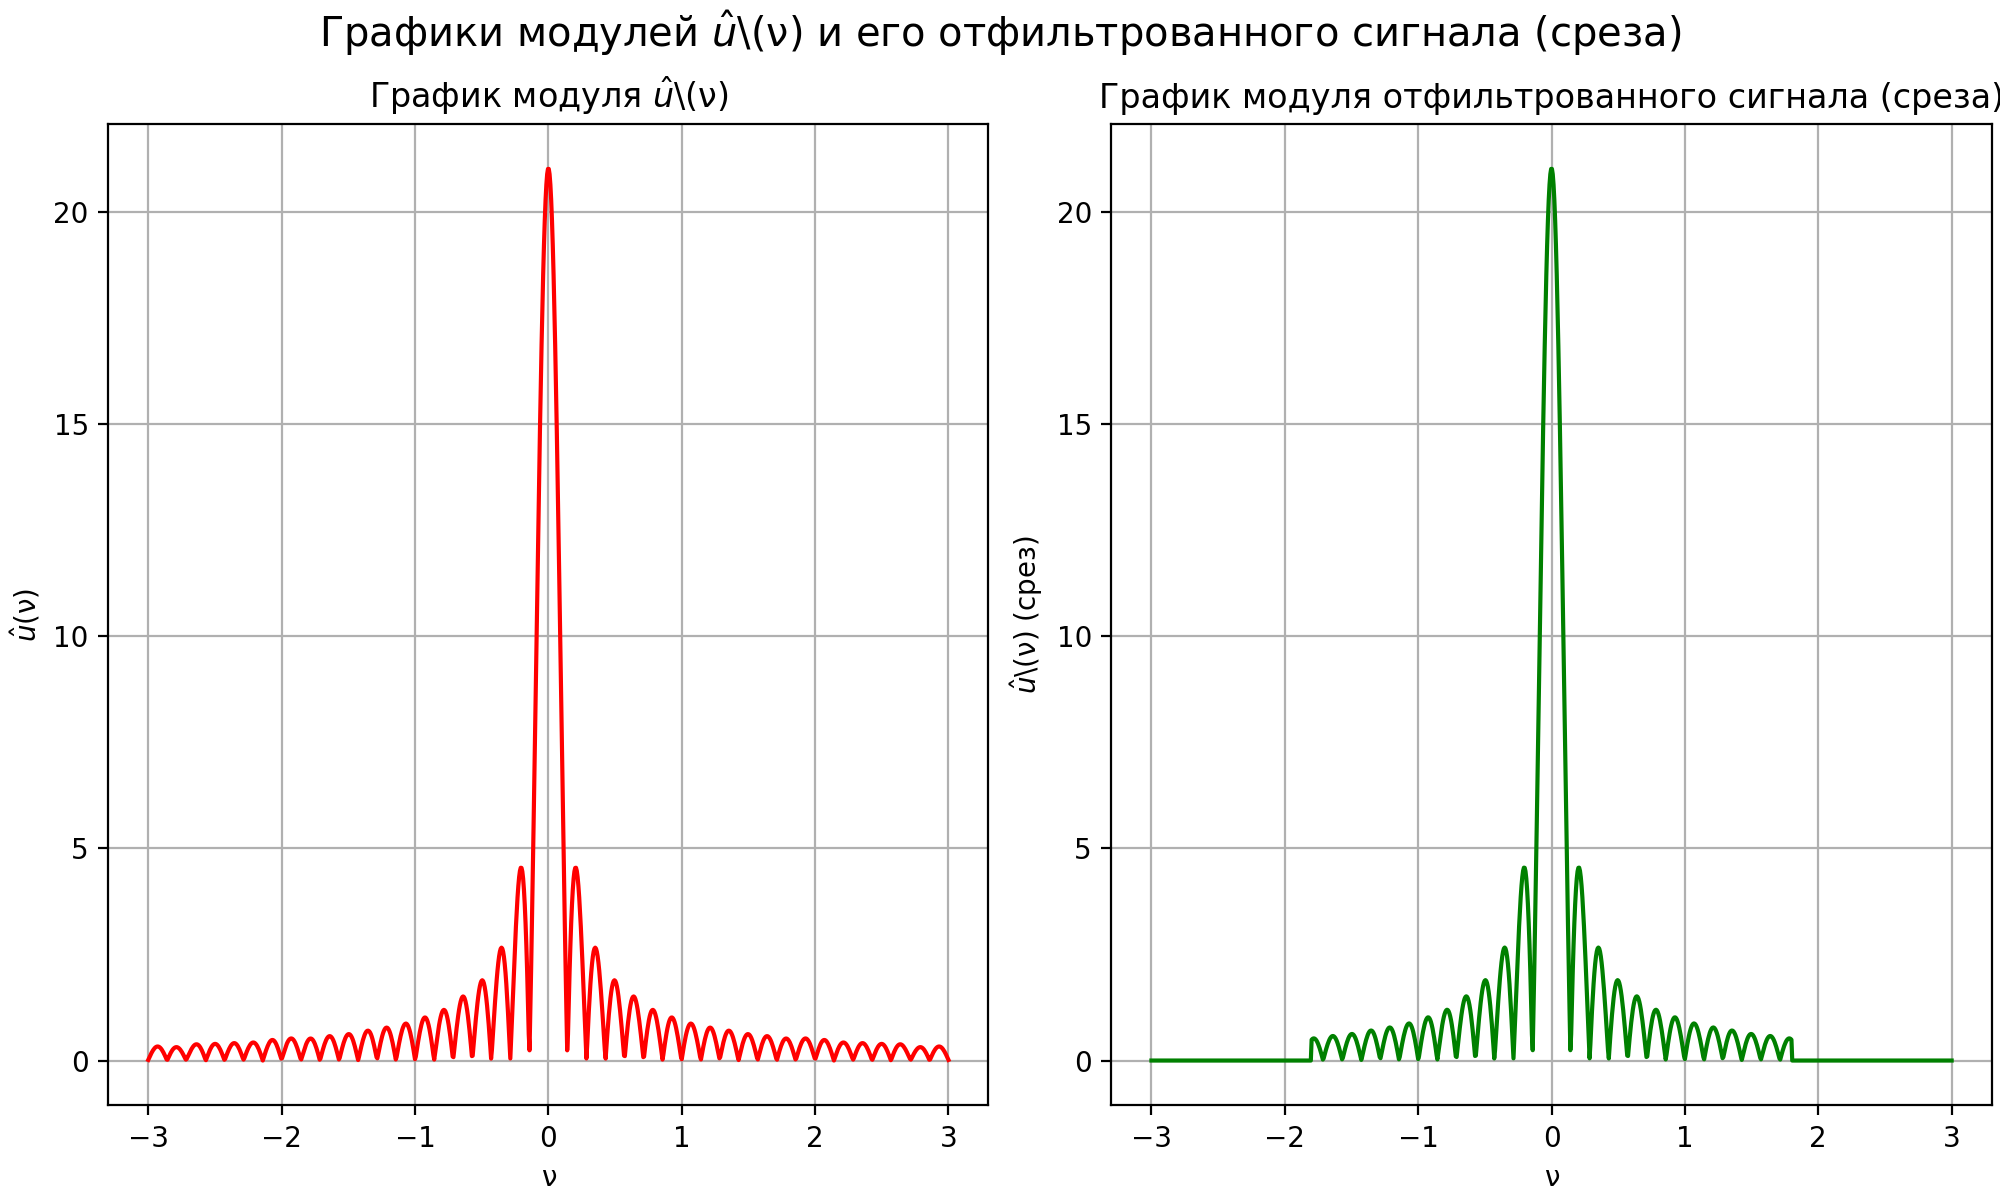
\includegraphics[scale=0.55]{media/1 task/high_freq/Fourier_Image_0,25_-1,7987987987987988.png}
    \caption{Графики модулей Фурье-образа $u(t)$ и отфильтрованного сигнала при $b=0.25$ и $\nu_0=1.8$ Гц}
    \label{fig:four_025_18}
\end{figure}

\begin{figure}[ht!]
    \centering
    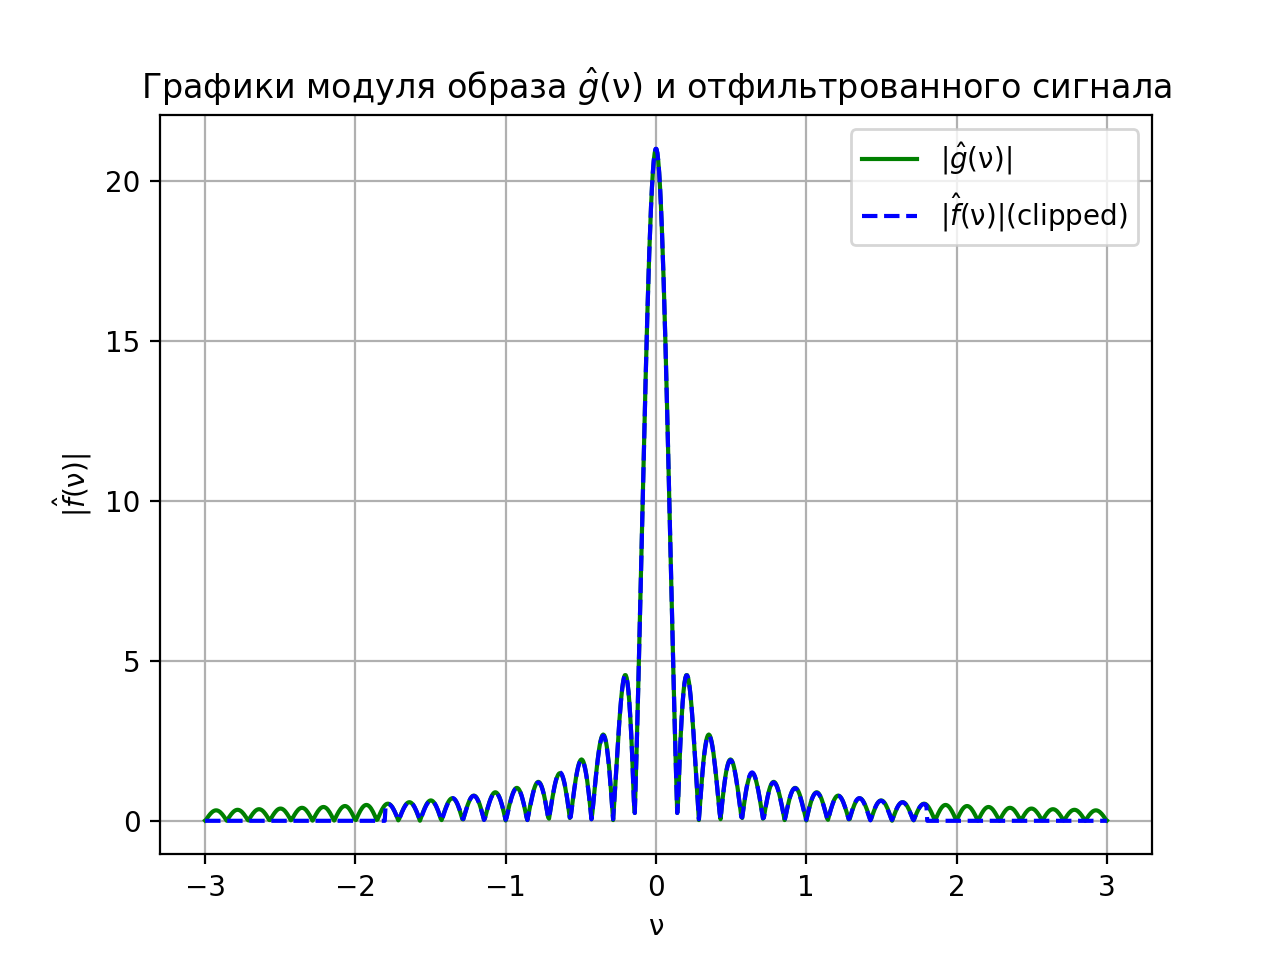
\includegraphics[scale=0.55]{media/1 task/high_freq/Fourier_Image_Comparison_0,25_-1,7987987987987988.png}
    \caption{Сравнительные графики модулей Фурье-образа $g(t)$ и отфильтрованного сигнала при $b=0.25$ и $\nu_0=1.8$ Гц}
    \label{fig:fourc_025_18}
\end{figure}

Выше были приведены графики для сигнала $u(t)$ при $b=0.25$, но с разными частотами среза. Это сделано для того, чтобы мы смогли узнать влияние частоты среза на отфильтрованный сигнал. Так что выполняем обратное преобразование Фурье <<обрезанного>> образа и сопоставляем полученный отфильтрованный сигнал с зашумленным и исходным:

\clearpage

\begin{figure}[ht!]
    \centering
    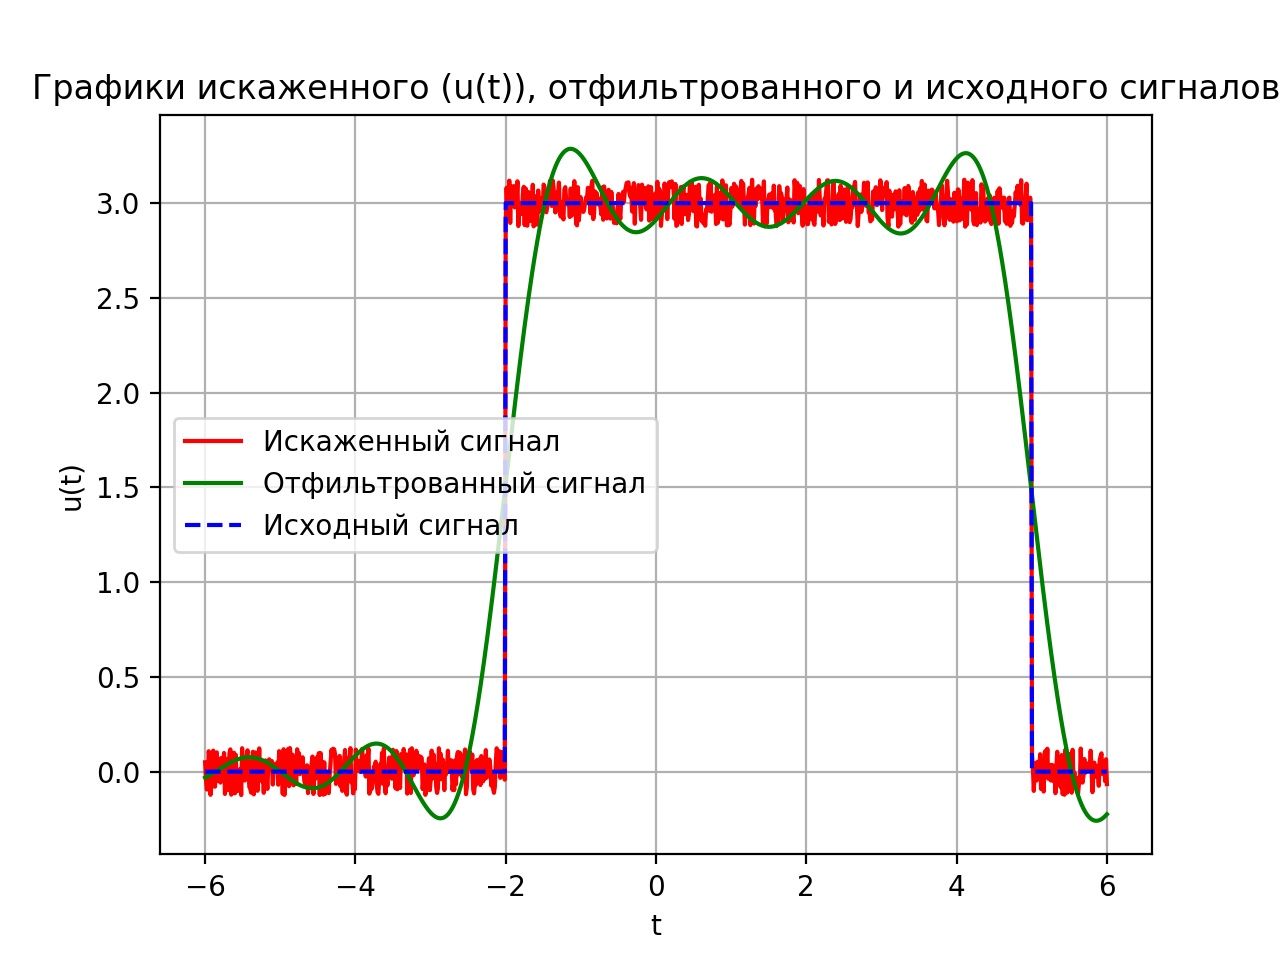
\includegraphics[scale=0.85]{media/1 task/high_freq/Cleaned_0,25_-0,5975975975975976.png}
    \caption{Графики  $u(t)$, отфильтрованного и исходного сигналов при $b=0.25$ и $\nu_0=0.6$ Гц}
    \label{fig:cleaned_025_06}
\end{figure}

\begin{figure}[ht!]
    \centering
    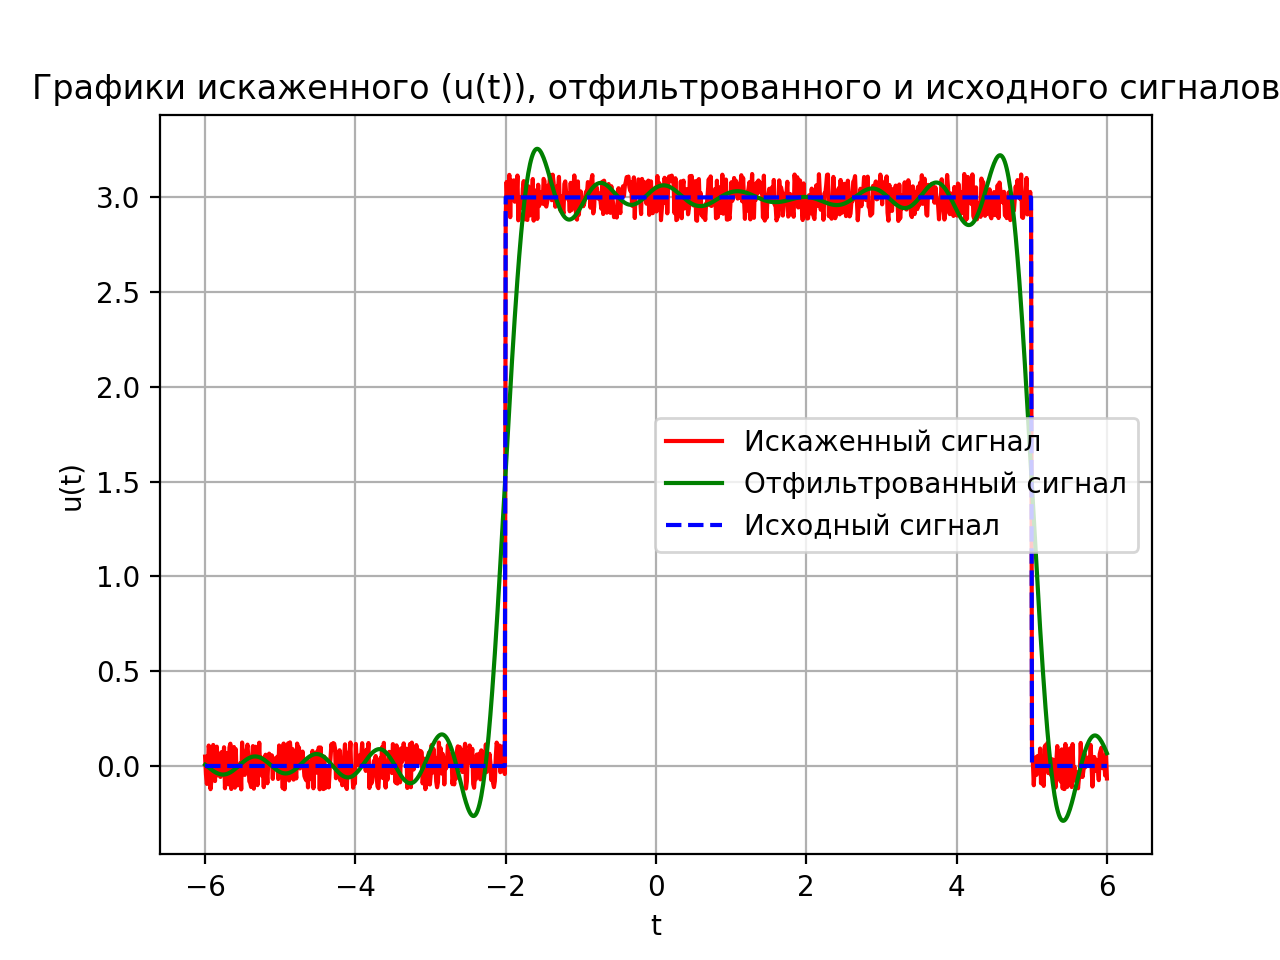
\includegraphics[scale=0.85]{media/1 task/high_freq/Cleaned_0,25_-1,1981981981981982.png}
    \caption{Графики  $u(t)$, отфильтрованного и исходного сигналов при $b=0.25$ и $\nu_0=1.2$ Гц}
    \label{fig:cleaned_025_12}
\end{figure}

\clearpage

\begin{figure}[ht!]
    \centering
    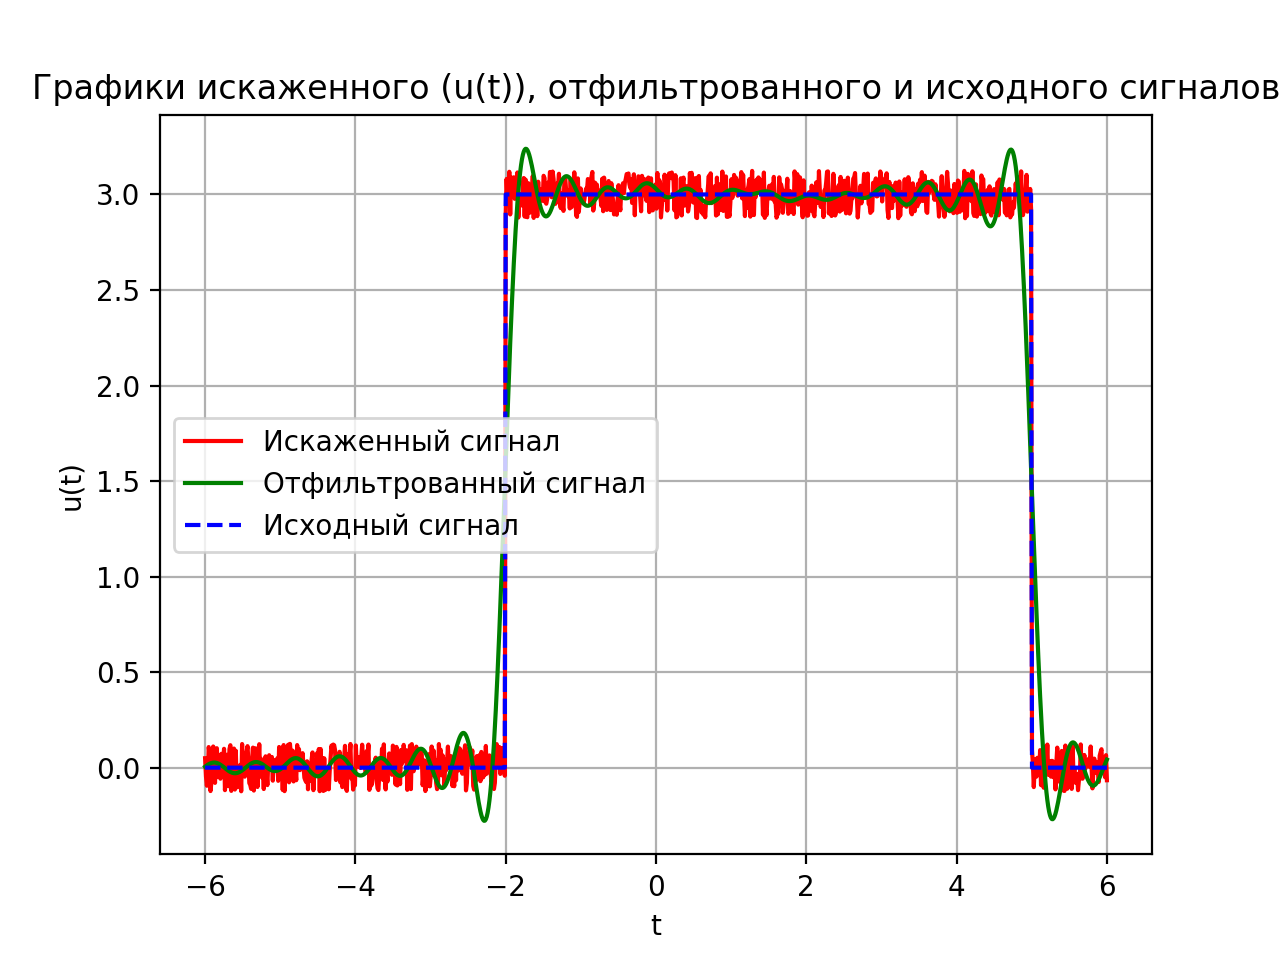
\includegraphics[scale=0.85]{media/1 task/high_freq/Cleaned_0,25_-1,7987987987987988.png}
    \caption{Графики  $u(t)$, отфильтрованного и исходного сигналов при $b=0.25$ и $\nu_0=1.8$ Гц} 
    \label{fig:cleaned_025_18}
\end{figure}

Из полученных графиков можно заключить, что при увеличении частоты среза отфильтрованный сигнал приближается к исходному по норме. В то же время увеличиваются колебания сигнала, что свидетельствует о большем влиянии хаотического шума. При меньшей частоте среза колебания (шумы) уменьшаются, но при этом функция становится более искажённой: сведение к минимуму влияния шума приводит к тому, что мы теряем часть высокочастотных компонент исходного сигнала.

Теперь зафиксируем частоту среза $\nu_0=1.2$ Гц и проанализируем влияние параметра $b$ на фильтрацию сигнала. Строим графики модулей Фурье-образов сигнала $u(t)$ и отфильтрованного сигнала, а также сравнительные графики модулей $g(t)$ и отфильтрованного сигнала при разных значениях $b$:



\begin{figure}[ht!]
    \centering
    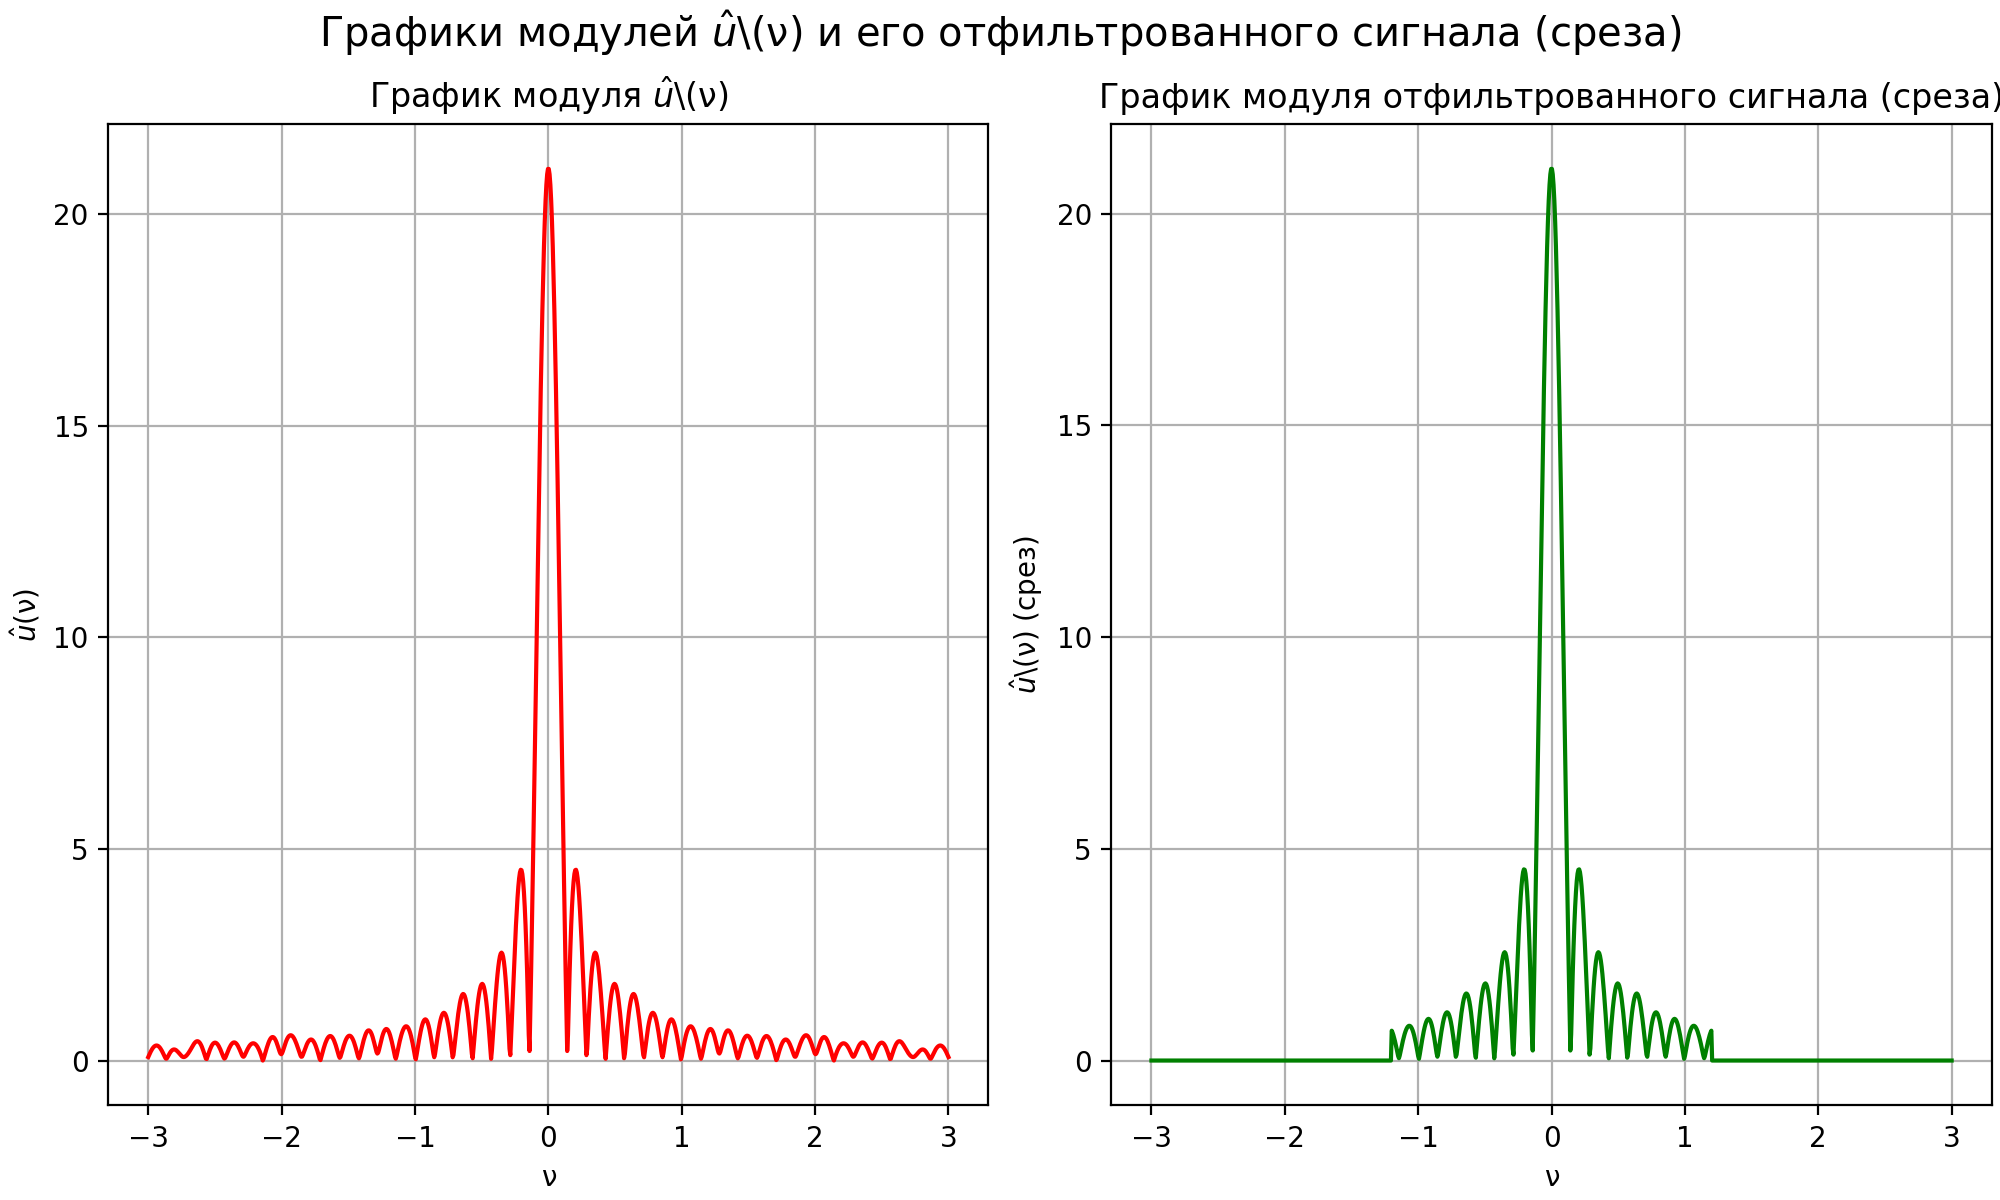
\includegraphics[scale=0.55]{media/1 task/high_freq/Fourier_Image_1_-1,1981981981981982.png}
    \caption{Графики модулей Фурье-образа $u (t)$ и отфильтрованного сигнала при $b=1$ и $\nu_0=1.2$ Гц}
    \label{fig:four_1_12}
\end{figure}

\begin{figure}[ht!]
    \centering
    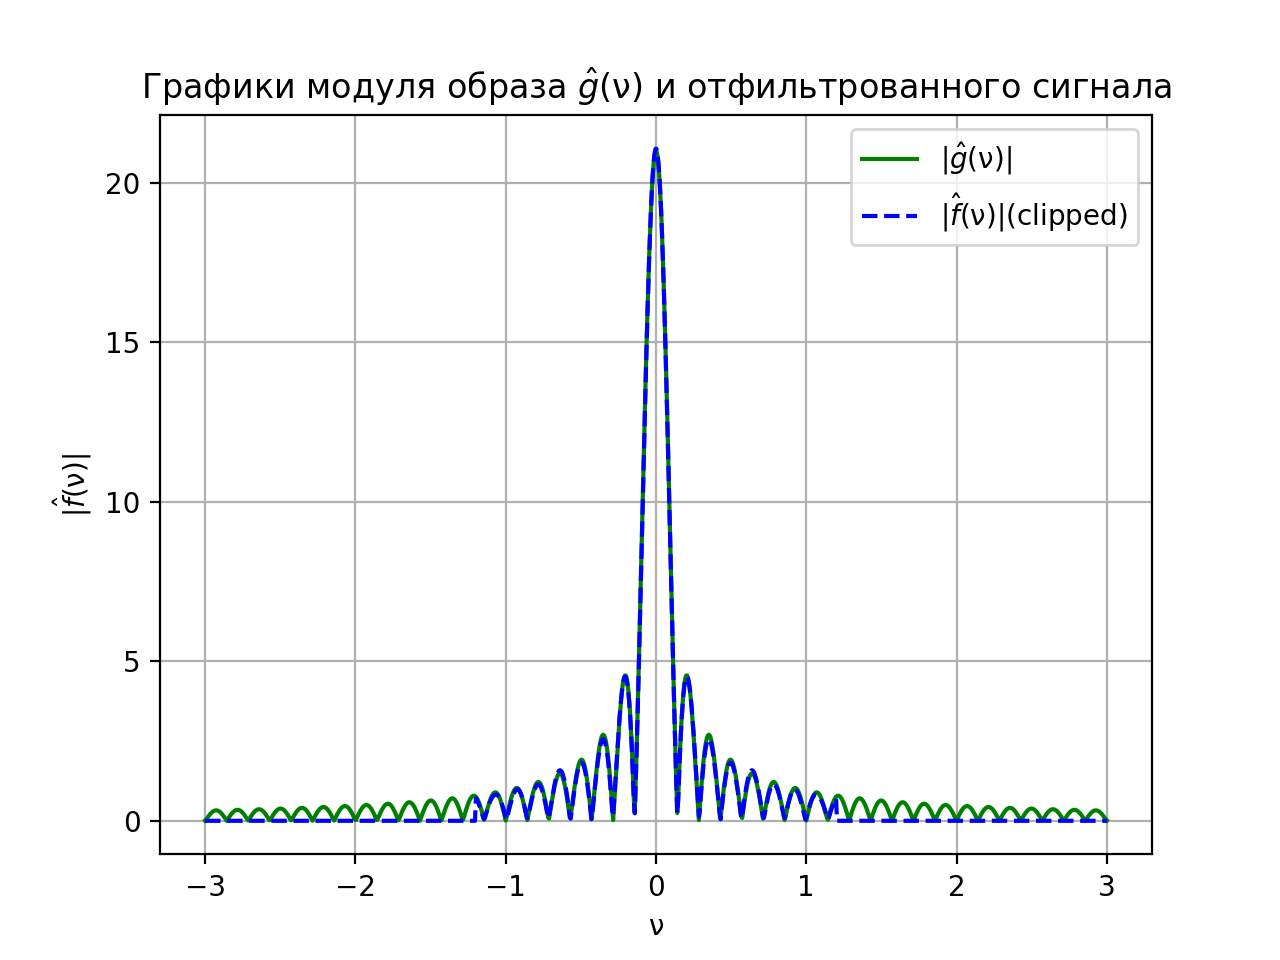
\includegraphics[scale=0.55]{media/1 task/high_freq/Fourier_Image_Comparison_1_-1,1981981981981982.png}
    \caption{Сравнительные графики модулей Фурье-образа $g(t)$ и отфильтрованного сигнала при $b=1$ и $\nu_0=1.2$ Гц}
    \label{fig:fourc_1_12}
\end{figure}

\begin{figure}[ht!]
    \centering
    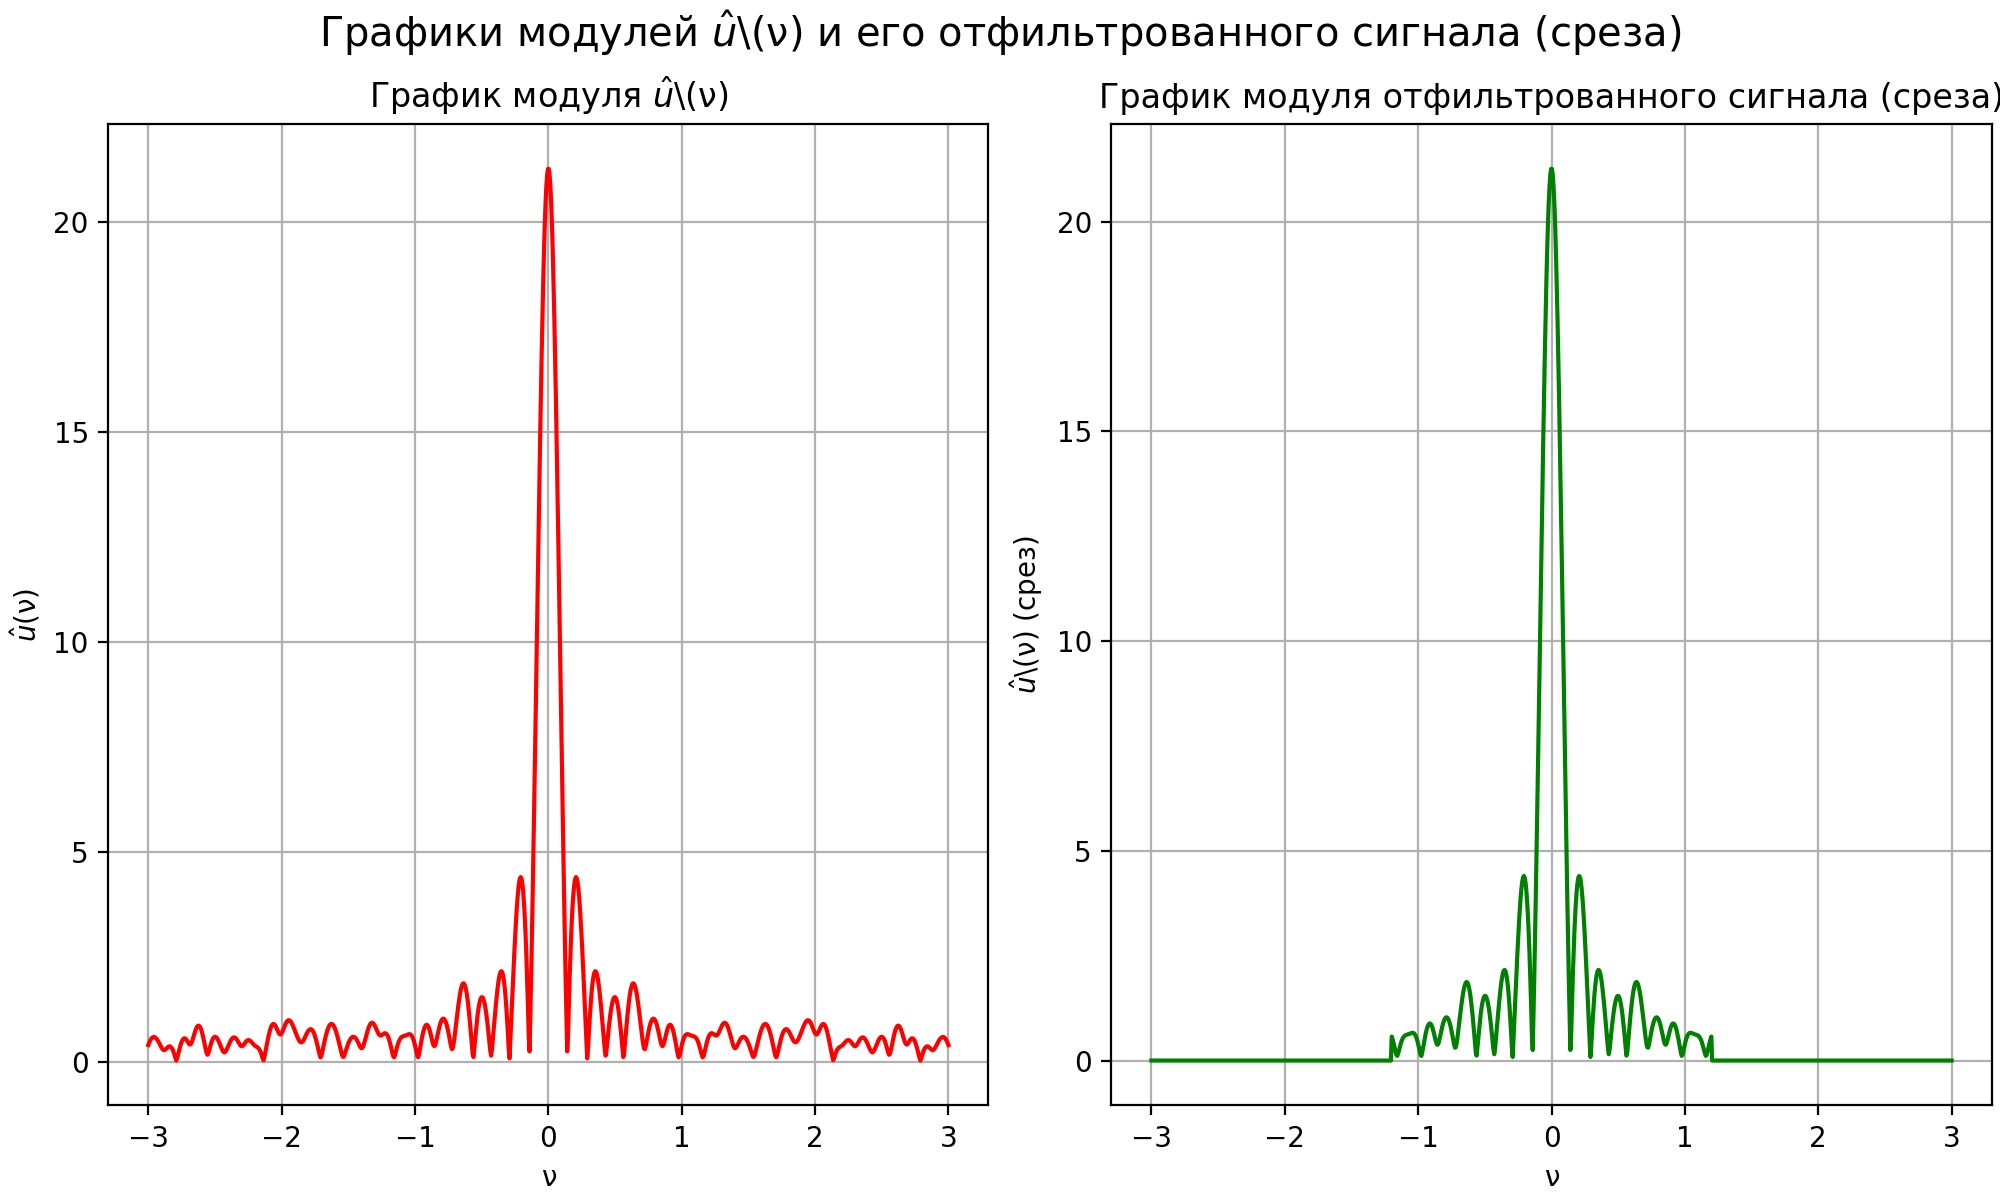
\includegraphics[scale=0.55]{media/1 task/high_freq/Fourier_Image_4_-1,1981981981981982.png}
    \caption{Графики модулей Фурье-образа $u(t)$ и отфильтрованного сигнала при $b=4$ и $\nu_0=1.2$ Гц}
    \label{fig:four_4_12}
\end{figure}

\begin{figure}[ht!]
    \centering
    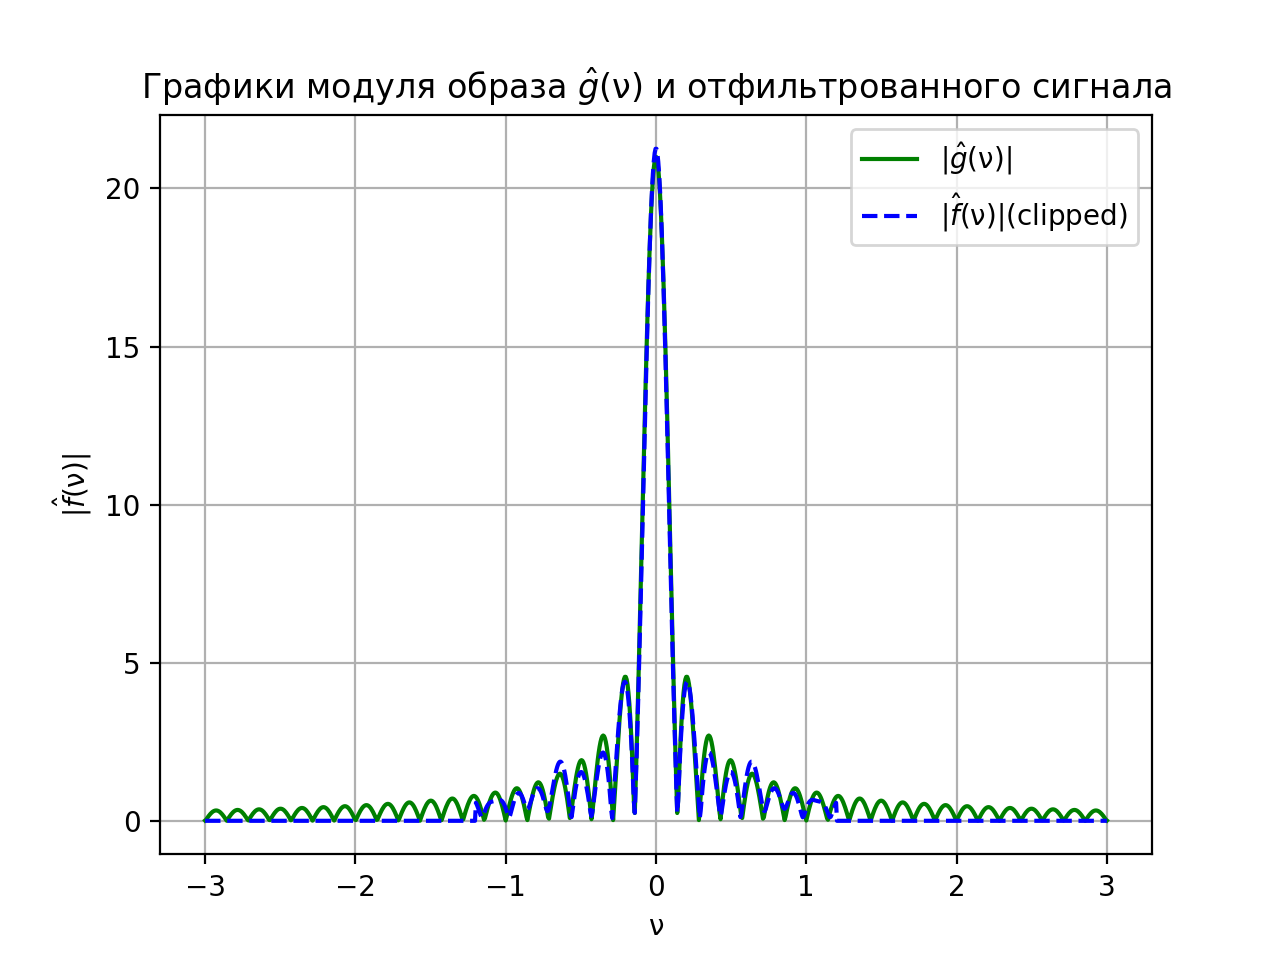
\includegraphics[scale=0.55]{media/1 task/high_freq/Fourier_Image_Comparison_4_-1,1981981981981982.png}
    \caption{Сравнительные графики модулей Фурье-образа $g(t)$ и отфильтрованного сигнала при $b=4$ и $\nu_0=1.2$ Гц}
    \label{fig:fourc_4_12}
\end{figure}

\clearpage

Графики зашумленного, отфильтрованного и исходного сигналов:

\begin{figure}[ht!]
    \centering
    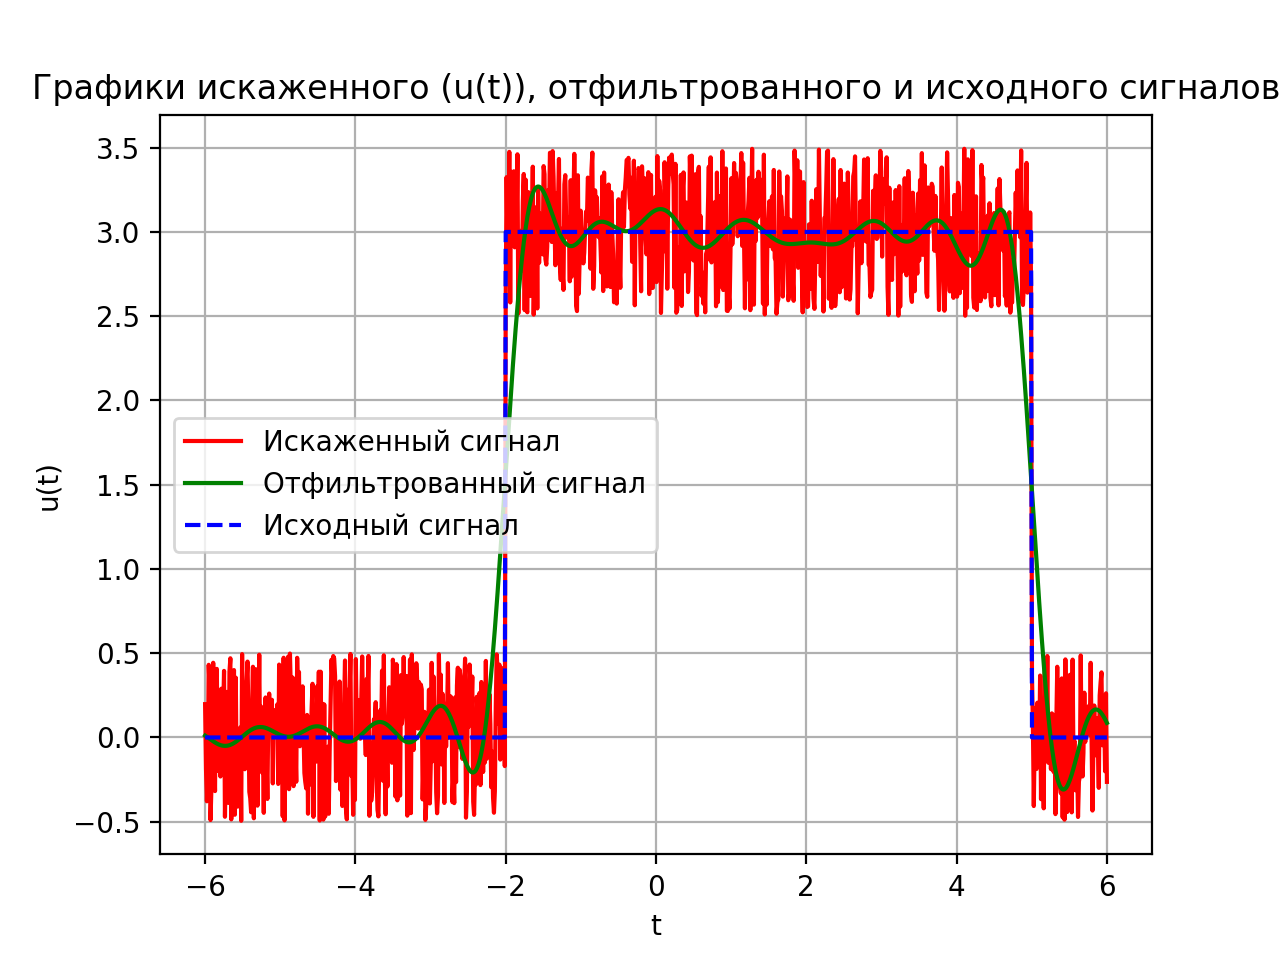
\includegraphics[scale=0.85]{media/1 task/high_freq/Cleaned_1_-1,1981981981981982.png}
    \caption{Графики  $u(t)$, отфильтрованного и исходного сигналов при $b=1$ и $\nu_0=1.2$ Гц} 
    \label{fig:cleaned_1_12}
\end{figure}

\begin{figure}[ht!]
    \centering
    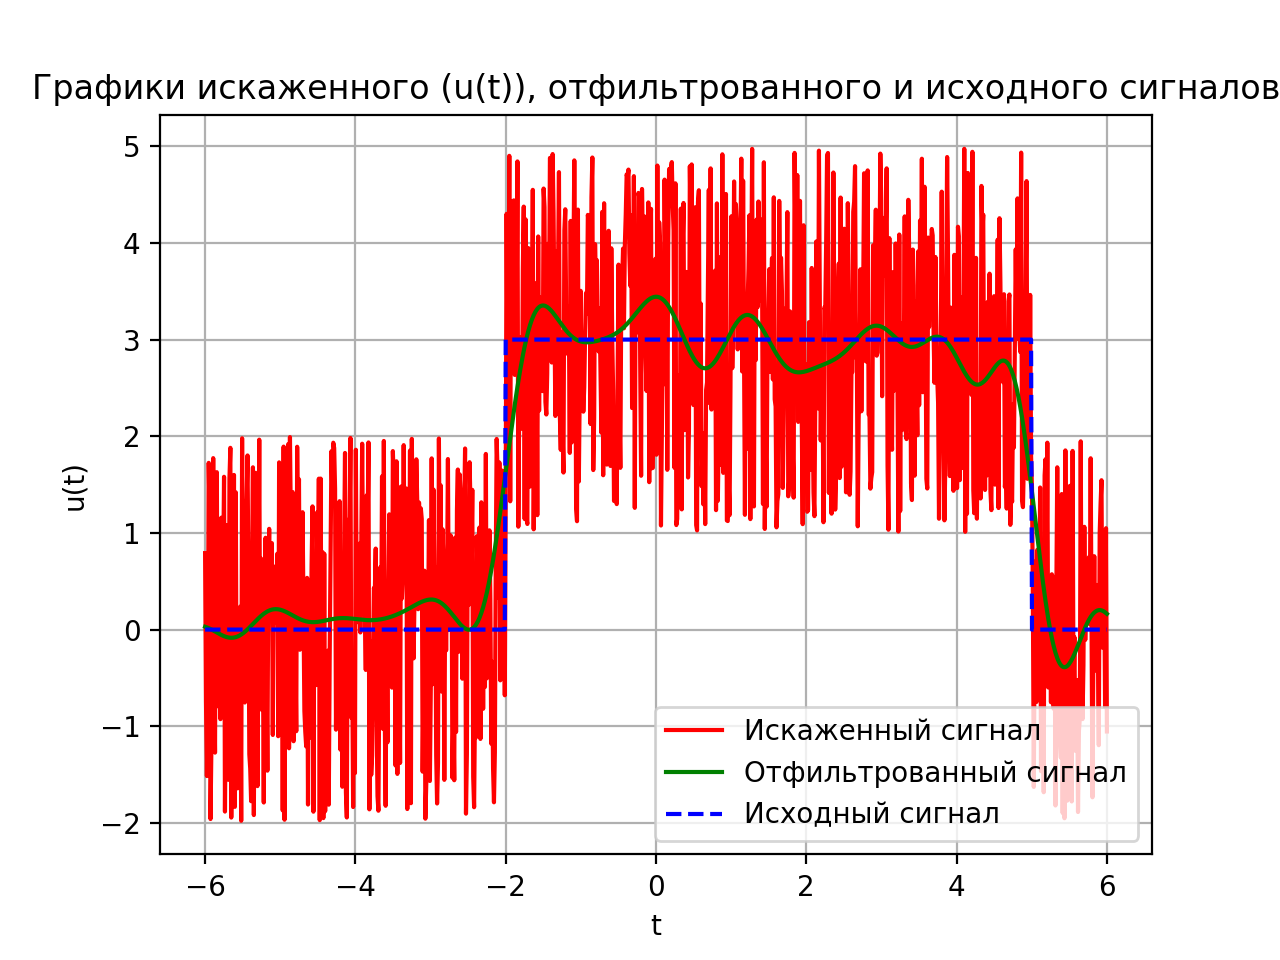
\includegraphics[scale=0.85]{media/1 task/high_freq/Cleaned_4_-1,1981981981981982.png}
    \caption{Графики  $u(t)$, отфильтрованного и исходного сигналов при $b=4$ и $\nu_0=1.2$ Гц}
    \label{fig:cleaned_4_12}
\end{figure}

Обратим внимание на модули Фурье-образов при значениях $0.25, 1, 4$ параметра $b$ (рисунки \ref{fig:four_025_12}, \ref{fig:four_1_12} и \ref{fig:four_4_12} соответственно). Стоит отметить, что при увеличении значения графики модуля Фурье-образа становятся более хаотичным при высоких частотах. Это свидетельствует о том, что увеличивается влияние высокочастотного шума на сигнал $u(t)$. Далее перейдём к графикам отфильтрованного сигнала (рисунки \ref{fig:cleaned_025_12}, \ref{fig:cleaned_1_12}, \ref{fig:cleaned_4_12}). При увеличении параметра уменьшается приближение отфильтрованного сигнала к исходному по норме, что является признаком большего влияния высокочастотного шума на сигнал. Однако это приводит к тому, что при большем значении $b$ отфильтрованный сигнал имеет меньше колебаний, так как высокочастотные компоненты Фурье-образа в большей степени вызваны искажением сигнала, а не природой исходной функции $g(t)$. 

\clearpage
\subsection{Специфические частоты}

Теперь мы будем оставлять значение лишь определённого диапазона частот при фильтрации. Это означает, что мы будем отбрасывать частоты таким образом, чтобы график модуля образа Фурье отфильтрованного сигнала как можно точнее совпадал с аналогичным графиком исходного сигнала $g(t)$. Для того, чтобы проанализировать влияние параметров на фильтрацию сигнала, мы для начала зафиксируем диапазон определённых частот, а затем рассмотрим влияние частот среза. В этом пункте параметры $c$ и $d$ будут ненулевыми.

\subsubsection{Рассматриваем зашумленные сигналы при $b=0$}\label{b_0}

Начнём наши ислледования при $b=0$. Строим графики аналогично пункту выше и анализируем их:

\begin{figure}[ht!]
    \centering
    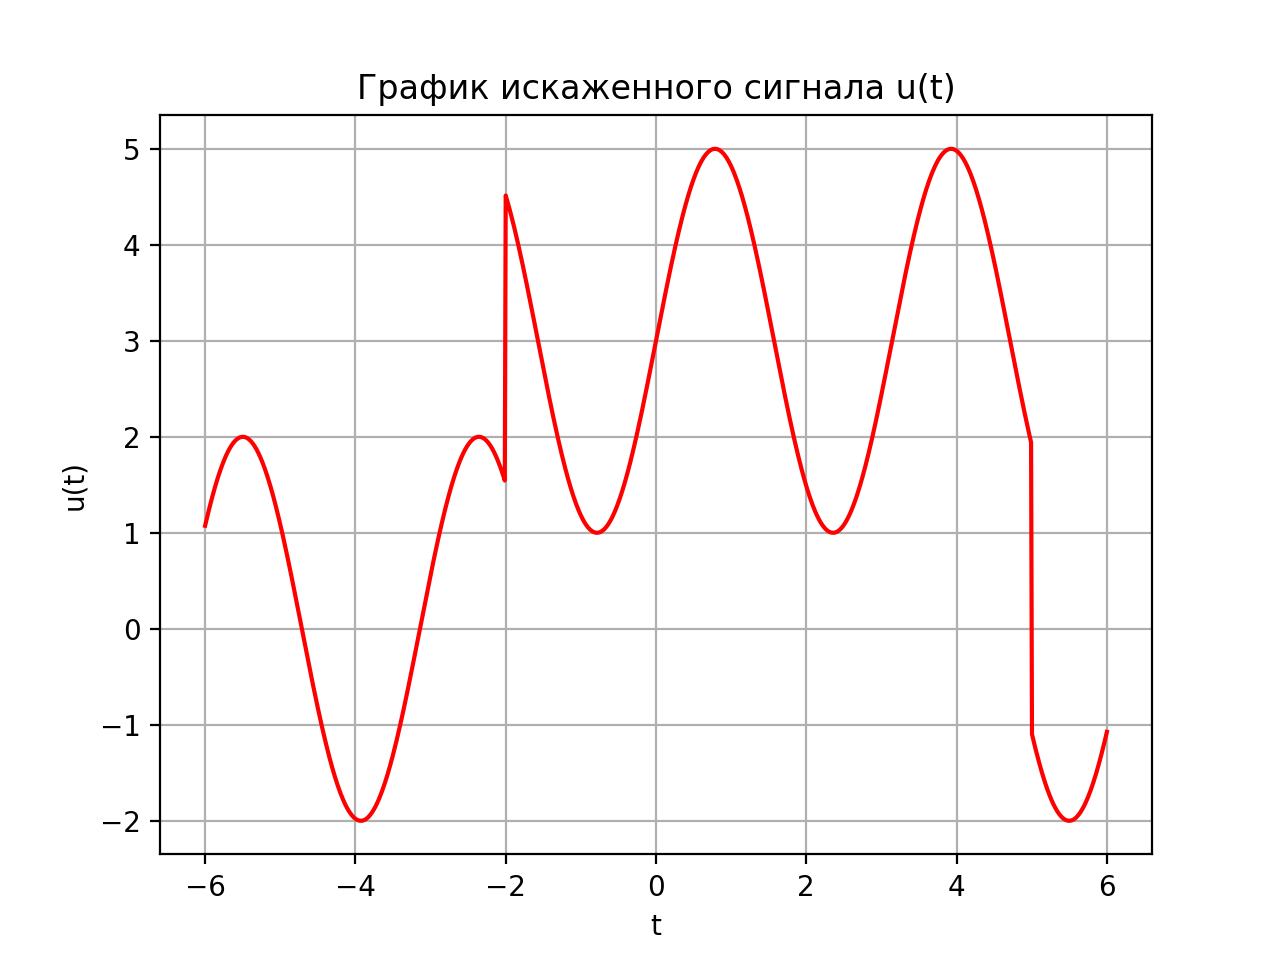
\includegraphics[scale=0.75]{media/1 task/specific_freq/Noisy_0_2_2.png}
    \caption{График функции $u(t)$ при $b=0$,  $c=2$,  $d=2$}
    \label{fig:noisy_0_2_2}
\end{figure}

\clearpage

\begin{figure}[ht!]
    \centering
    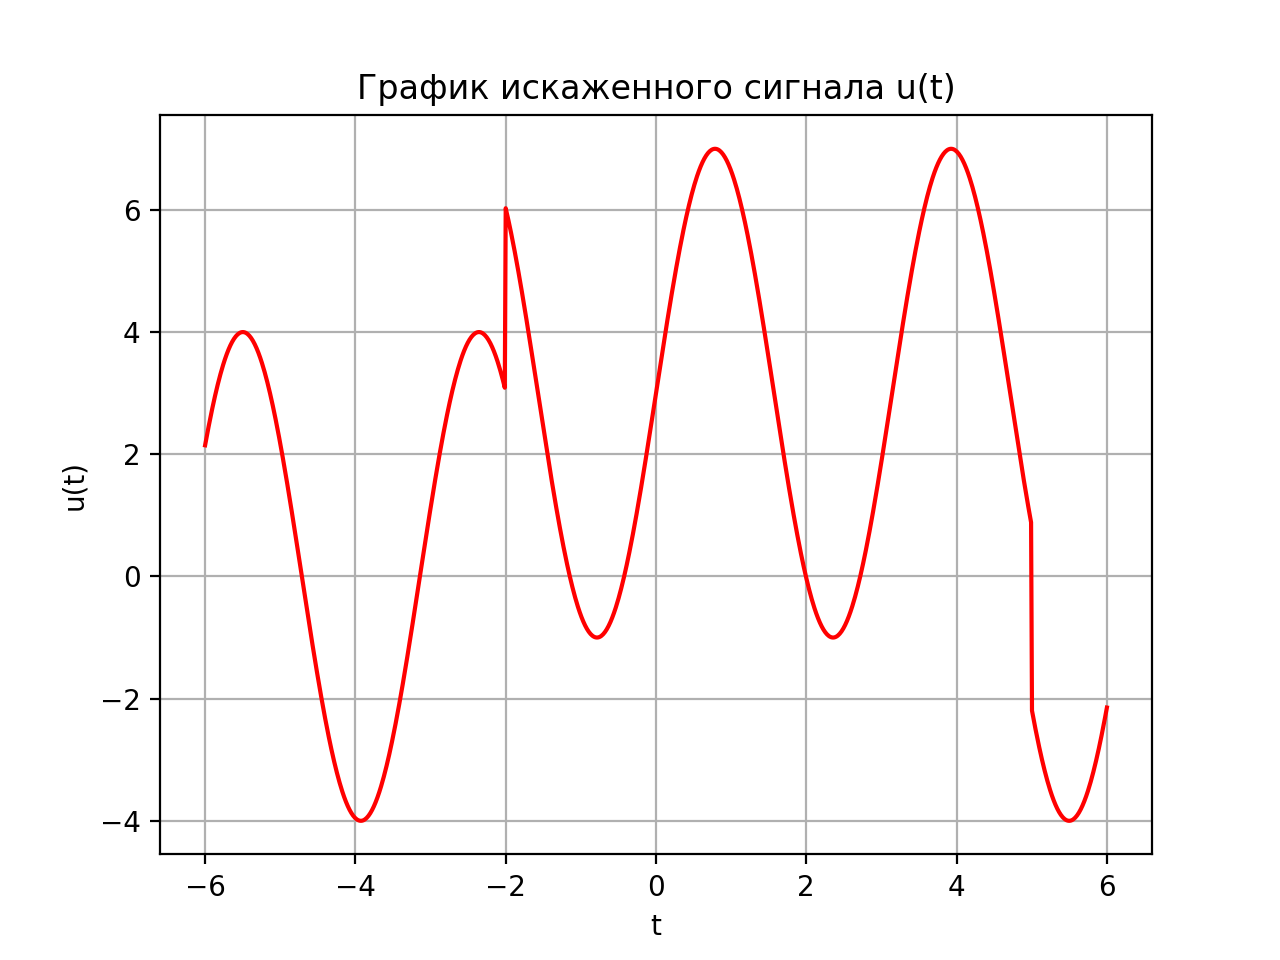
\includegraphics[scale=0.75]{media/1 task/specific_freq/Noisy_0_4_2.png}
    \caption{График функции $u(t)$ при $b=0$,  $c=4$,  $d=2$}
    \label{fig:noisy_0_4_2}
\end{figure}

\begin{figure}[ht!]
    \centering
    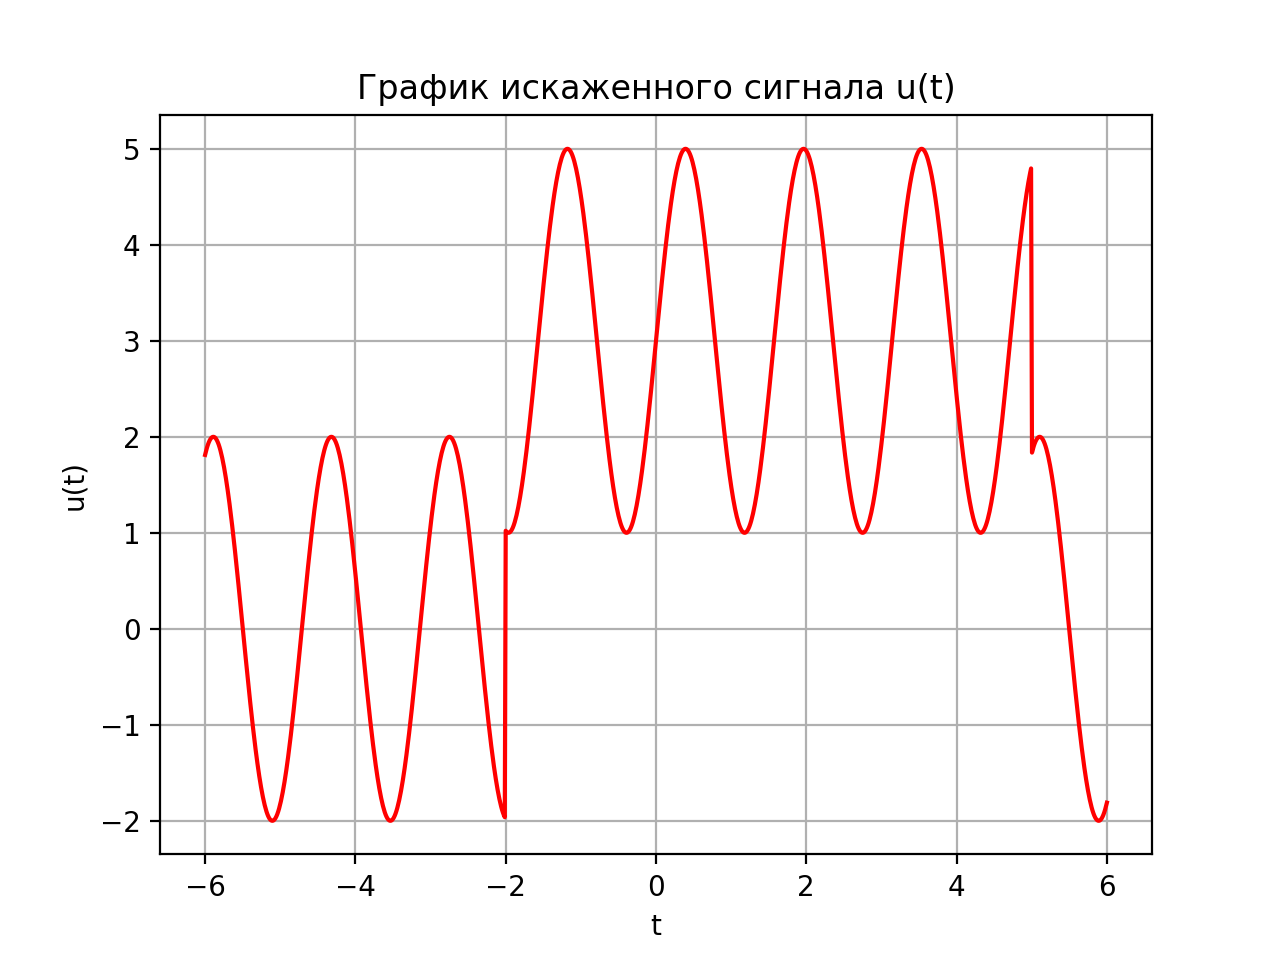
\includegraphics[scale=0.75]{media/1 task/specific_freq/Noisy_0_2_4.png}
    \caption{График функции $u(t)$ при $b=0$,  $c=2$,  $d=4$}
    \label{fig:noisy_0_2_4}
\end{figure}

На основе графиков можно сделать вывод, что параметр $c$ влияет на амплитуду зашумленного сигнала, параметр $d$ --- частоту сигнала. Теперь оценим влияние этих параметров на фильтрацию при исключении частот $\nu_0\in[0.156, 0.805]$:


\begin{figure}[ht!]
    \centering
    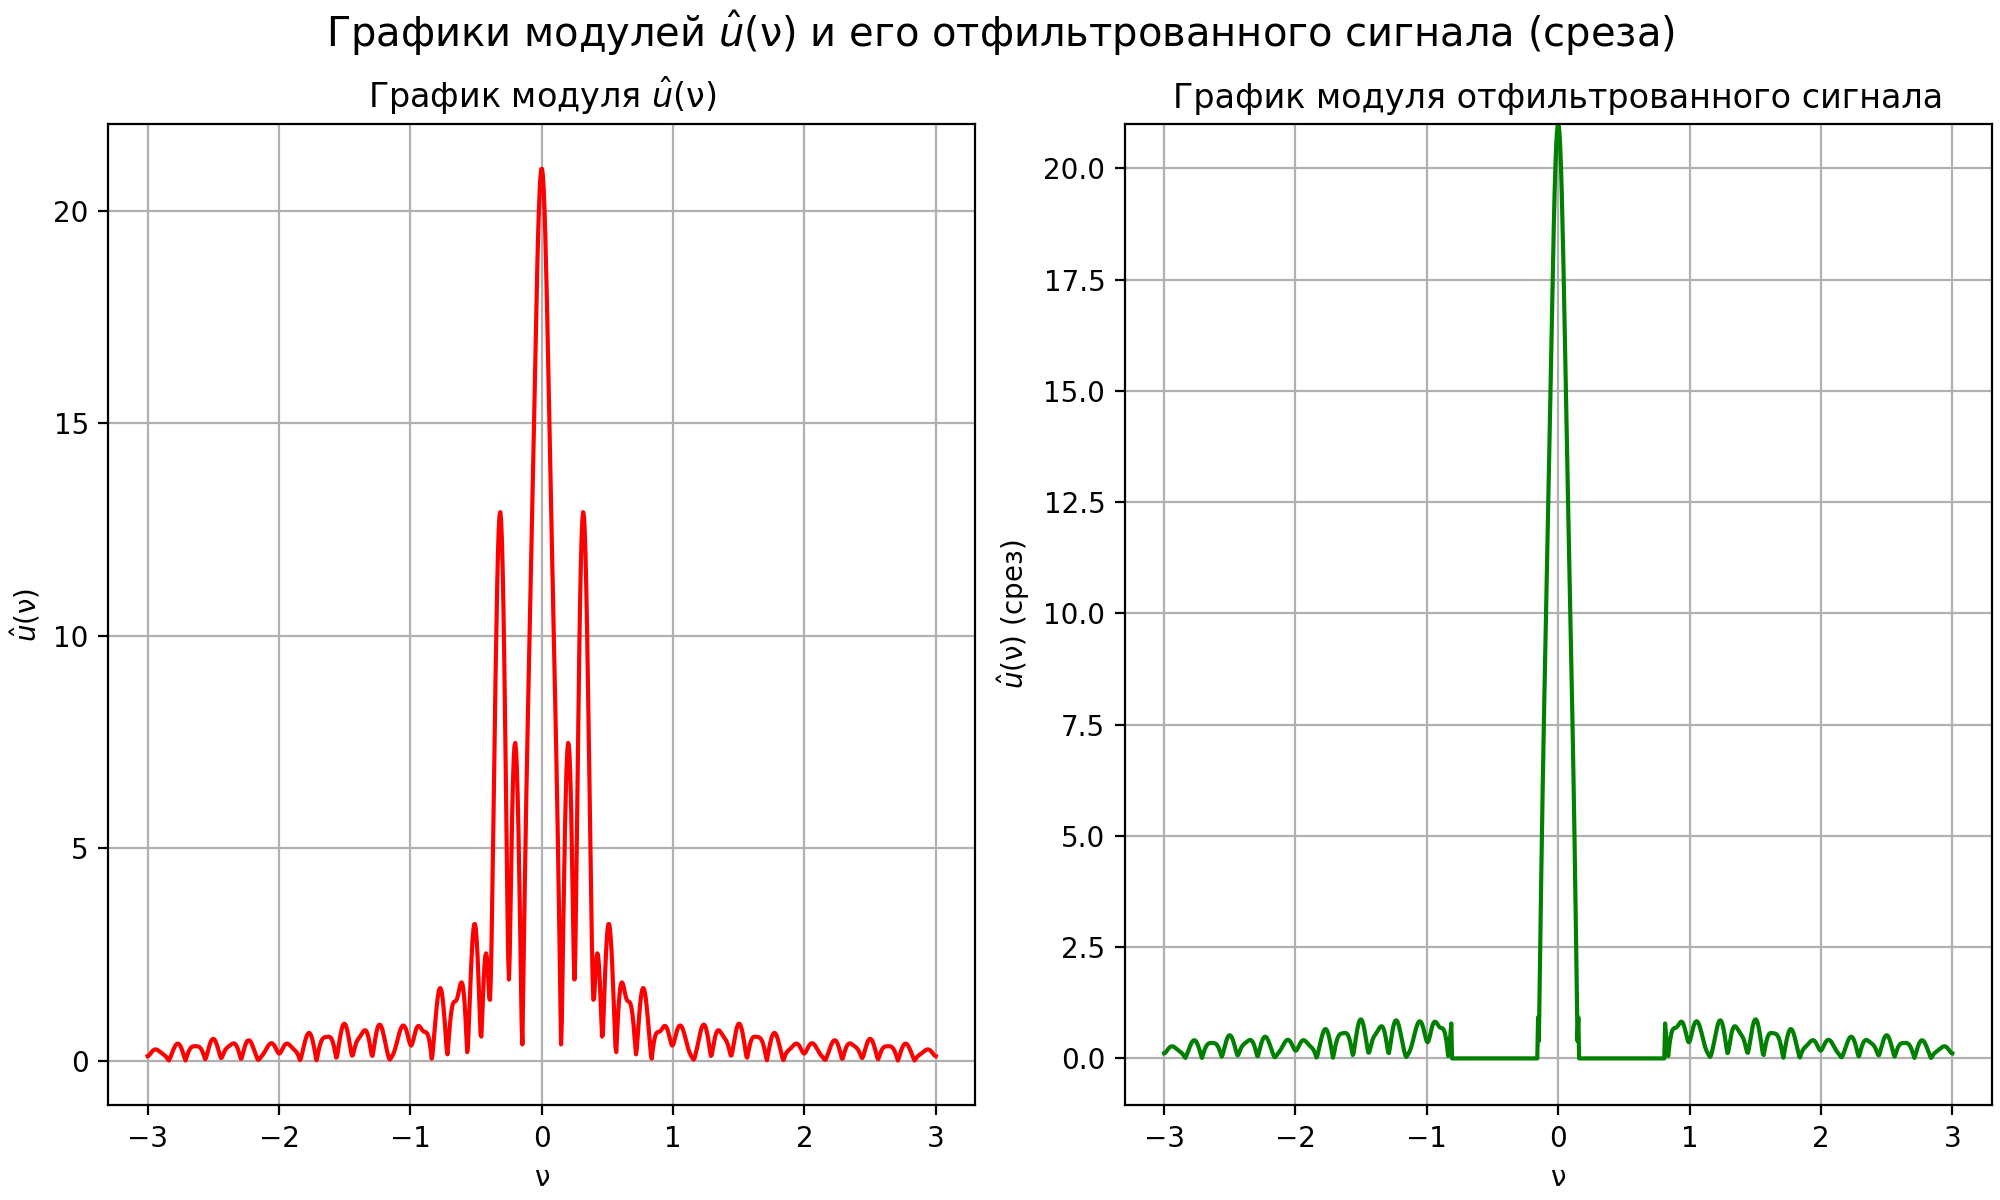
\includegraphics[scale=0.55]{media/1 task/specific_freq/Fourier_Image_0_2_2_-0,805:-0,156.png}
    \caption{Графики модулей Фурье-образа $u(t)$ и отфильтрованного сигнала при $b=0$,  $c=2$,  $d=2$}
    \label{fig:four_0_2_2}
\end{figure}

\begin{figure}[ht!]
    \centering
    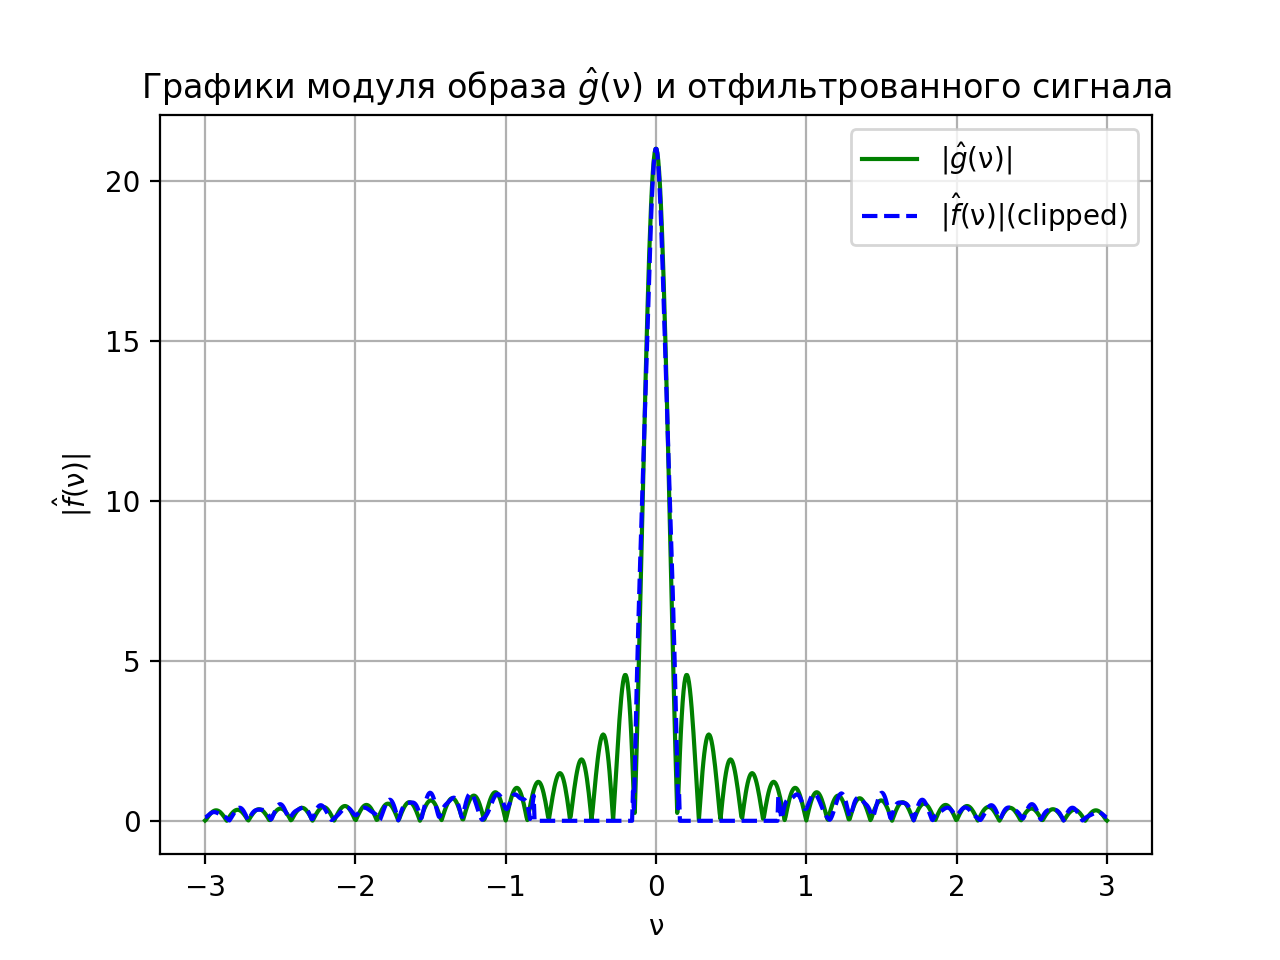
\includegraphics[scale=0.55]{media/1 task/specific_freq/Fourier_Image_Comparison_0_2_2_-0,805:-0,156.png}
    \caption{Сравнительные графики модулей Фурье-образа $g(t)$ и отфильтрованного сигнала при $b=0$,  $c=2$,  $d=2$}
    \label{fig:fourc_0_2_2}
\end{figure}

\begin{figure}[ht!]
    \centering
    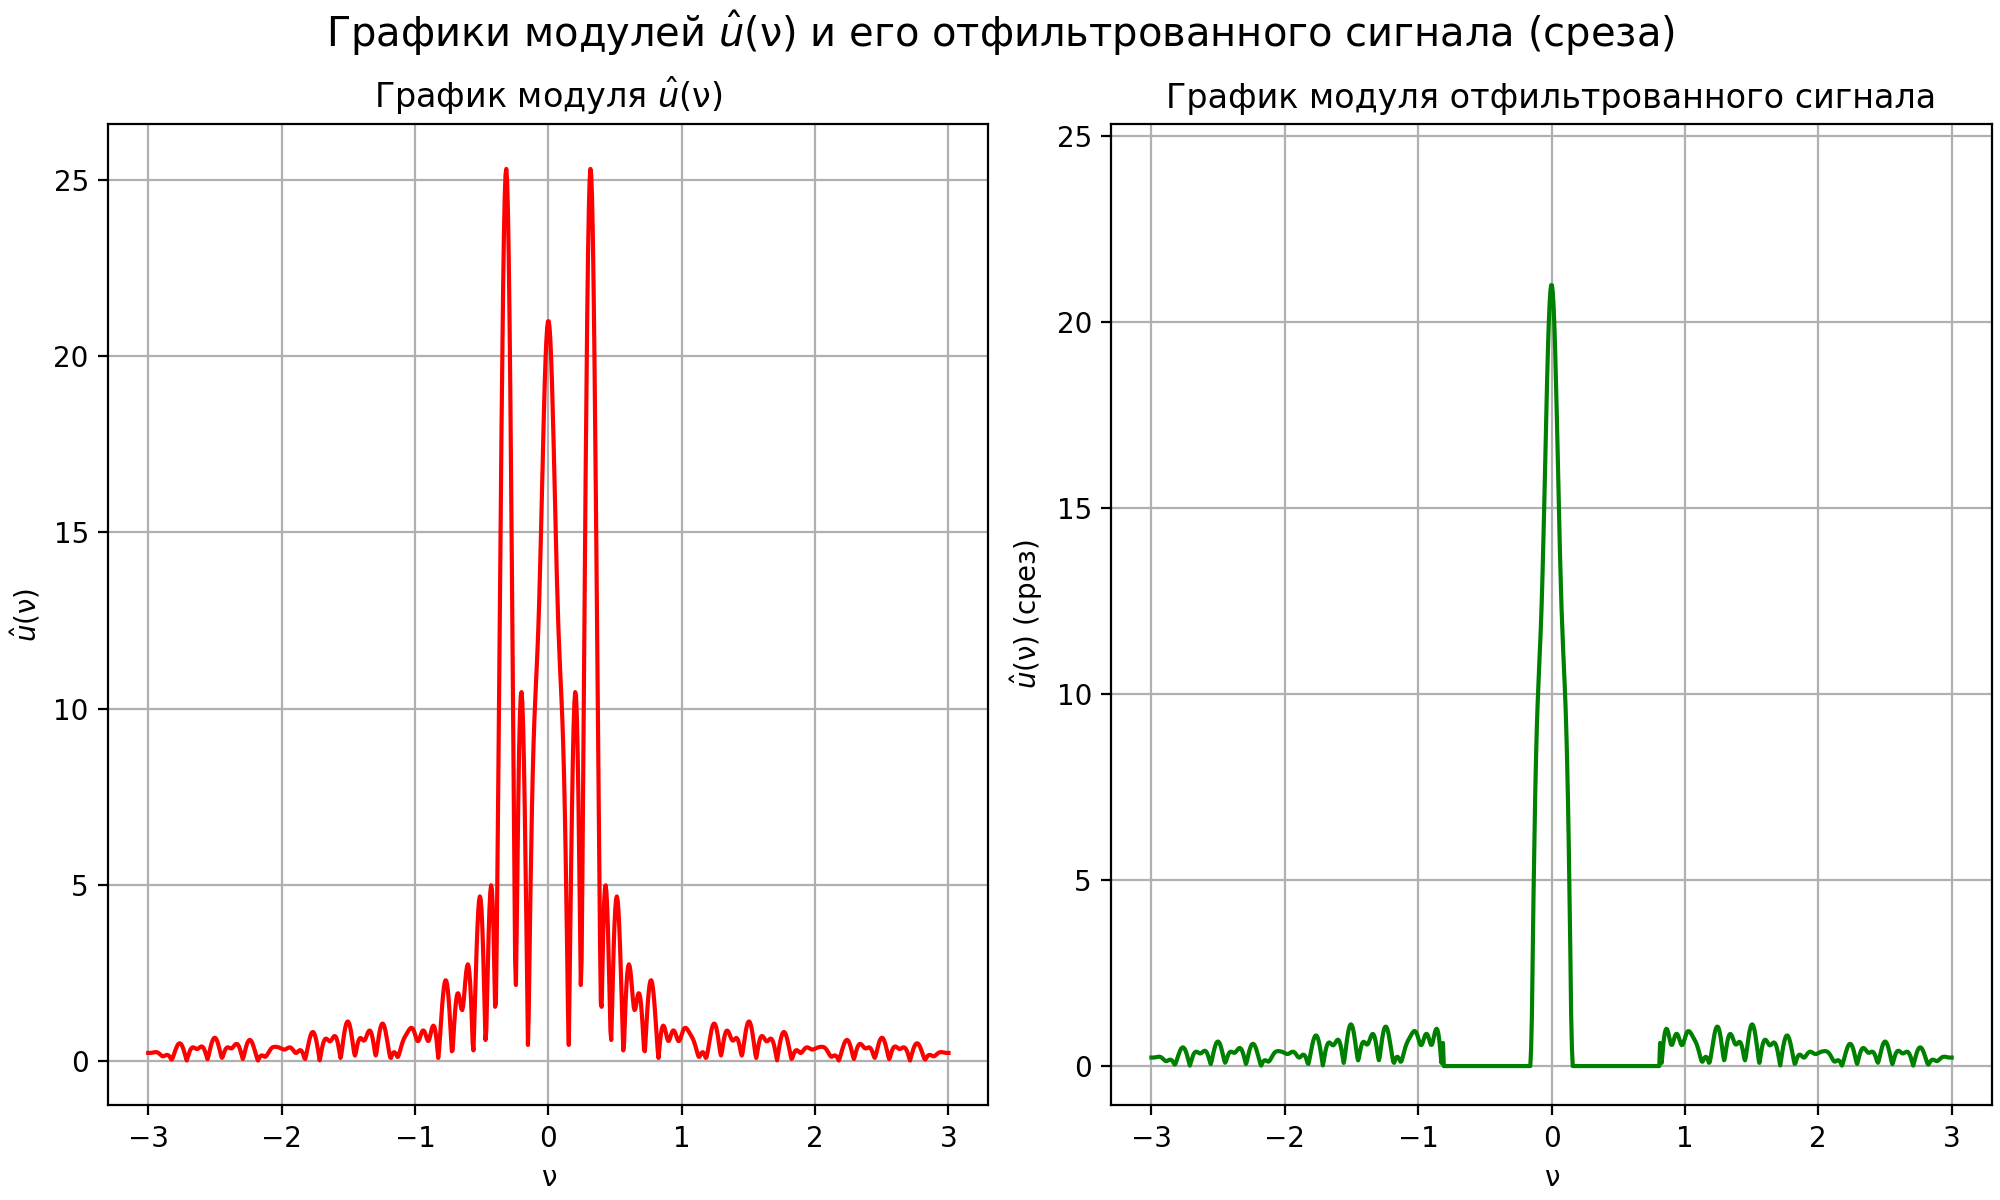
\includegraphics[scale=0.55]{media/1 task/specific_freq/Fourier_Image_0_4_2_-0,805:-0,156.png}
    \caption{Графики модулей Фурье-образа $u(t)$ и отфильтрованного сигнала при $b=0$,  $c=4$,  $d=2$}
    \label{fig:four_0_4_2}
\end{figure}

\begin{figure}[ht!]
    \centering
    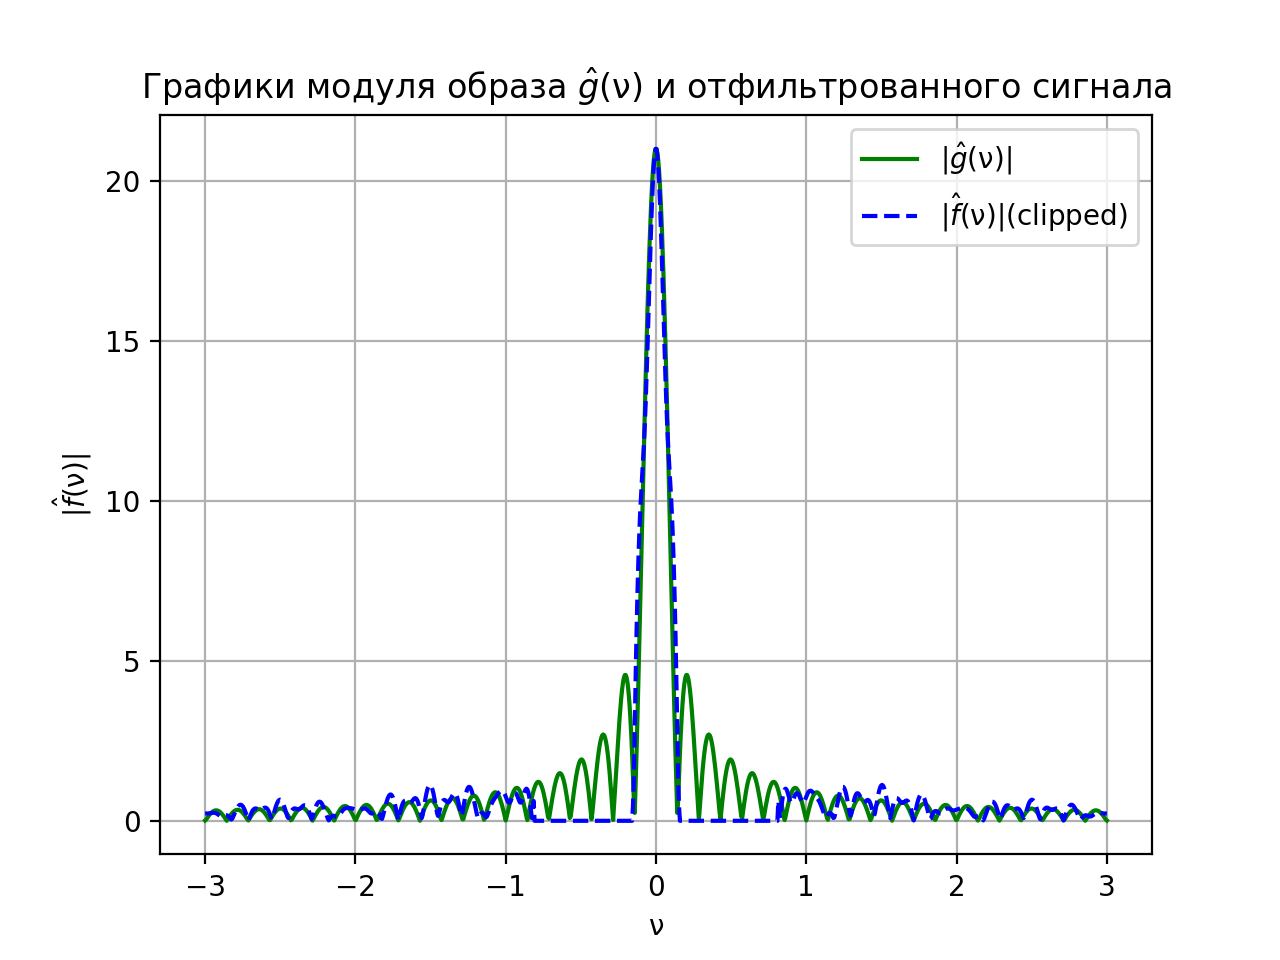
\includegraphics[scale=0.55]{media/1 task/specific_freq/Fourier_Image_Comparison_0_4_2_-0,805:-0,156.png}
    \caption{Сравнительные графики модулей Фурье-образа $g(t)$ и отфильтрованного сигнала при $b=0$,  $c=4$,  $d=2$}
    \label{fig:fourc_0_4_2}
\end{figure}

\clearpage

\begin{figure}[ht!]
    \centering
    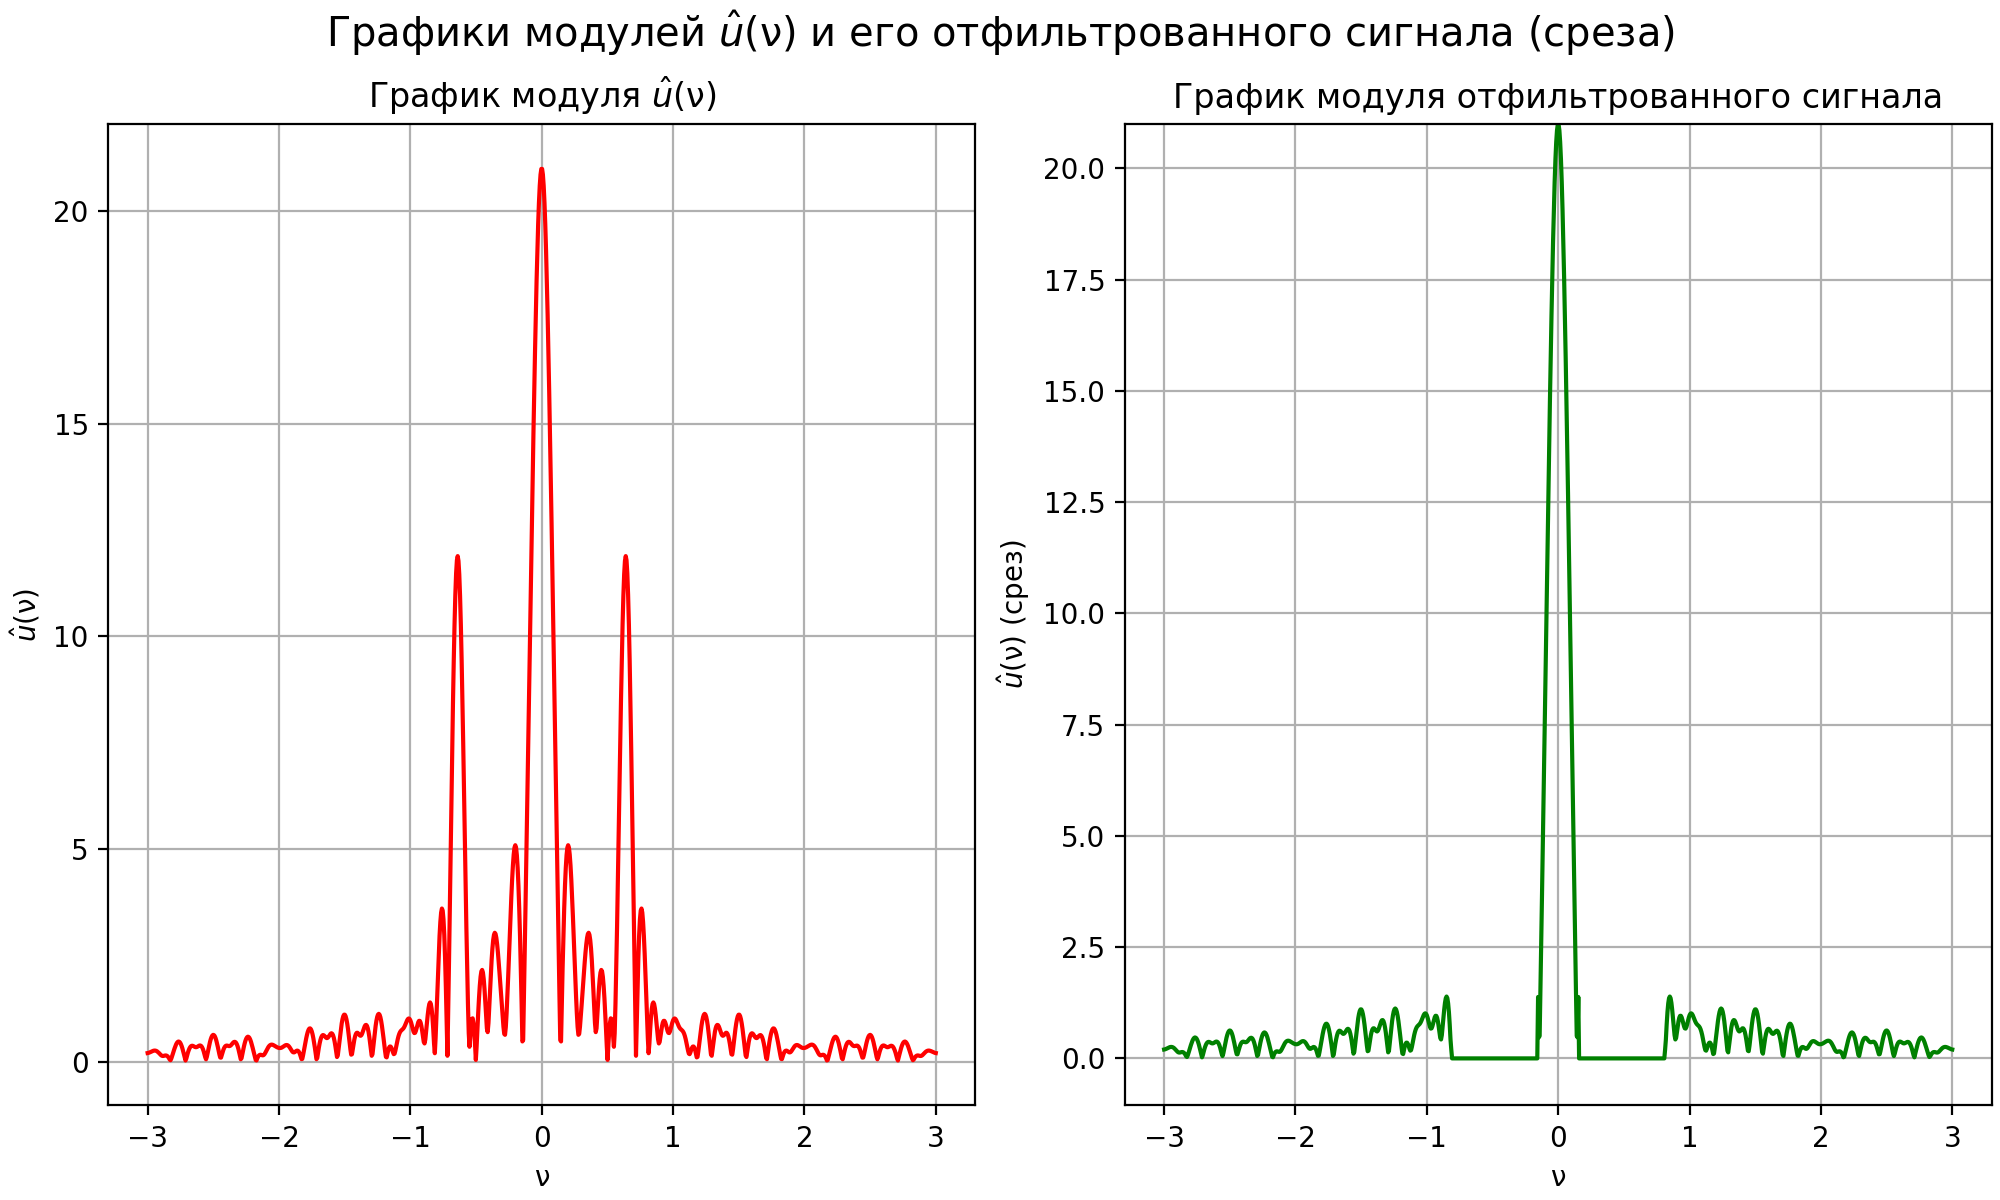
\includegraphics[scale=0.55]{media/1 task/specific_freq/Fourier_Image_0_2_4_-0,805:-0,156.png}
    \caption{Графики модулей Фурье-образа $f(t)$ и отфильтрованного сигнала при $b=0$,  $c=2$,  $d=4$}
    \label{fig:four_0_2_4}
\end{figure}

\begin{figure}[ht!]
    \centering
    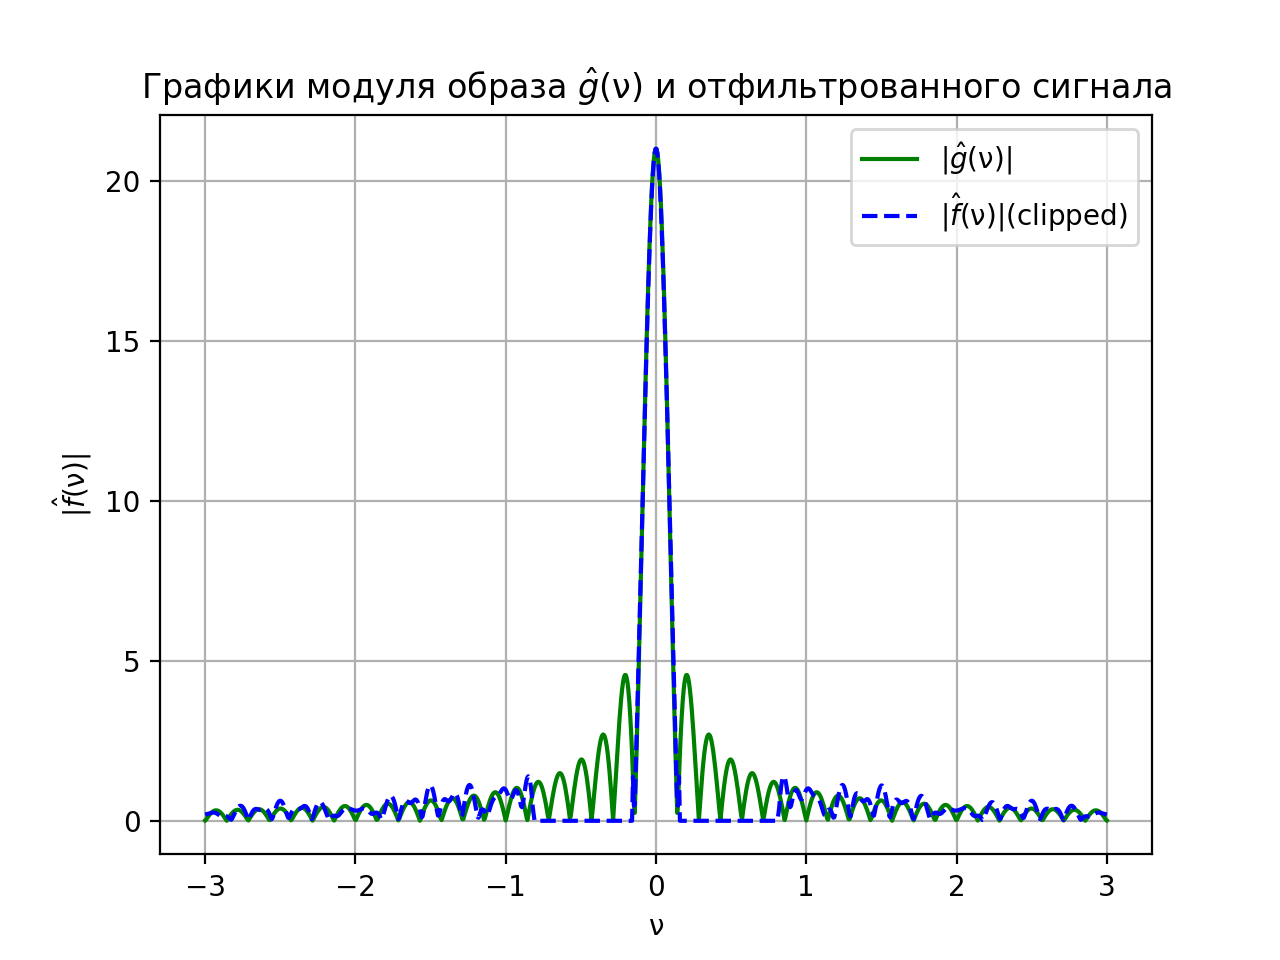
\includegraphics[scale=0.55]{media/1 task/specific_freq/Fourier_Image_Comparison_0_2_4_-0,805:-0,156.png}
    \caption{Сравнительные графики модулей Фурье-образа $g(t)$ и отфильтрованного сигнала при  $b=0$,  $c=2$,  $d=4$}
    \label{fig:fourc_0_2_4}
\end{figure}

Внимательно рассмотрев графики модулей Фурье-образов, можно прийти к выводу, что параметр $c$ прямо пропорционально влияет на значение модуля при частотах ниже $0.5$ Гц. Параметр $d$ при возрастании уменьшает влияние частот ниже 0.5 Гц и увеличивает влияние частот диапазона $\nu_0 \in[0.5, 1]$. При этом оба параметра увеличивают шум графика модуля образа Фурье для интервала остальных частот. Подобные выводы можно также сделать, взглянув на функцию $g(t)$.

\begin{figure}[ht!]
    \centering
    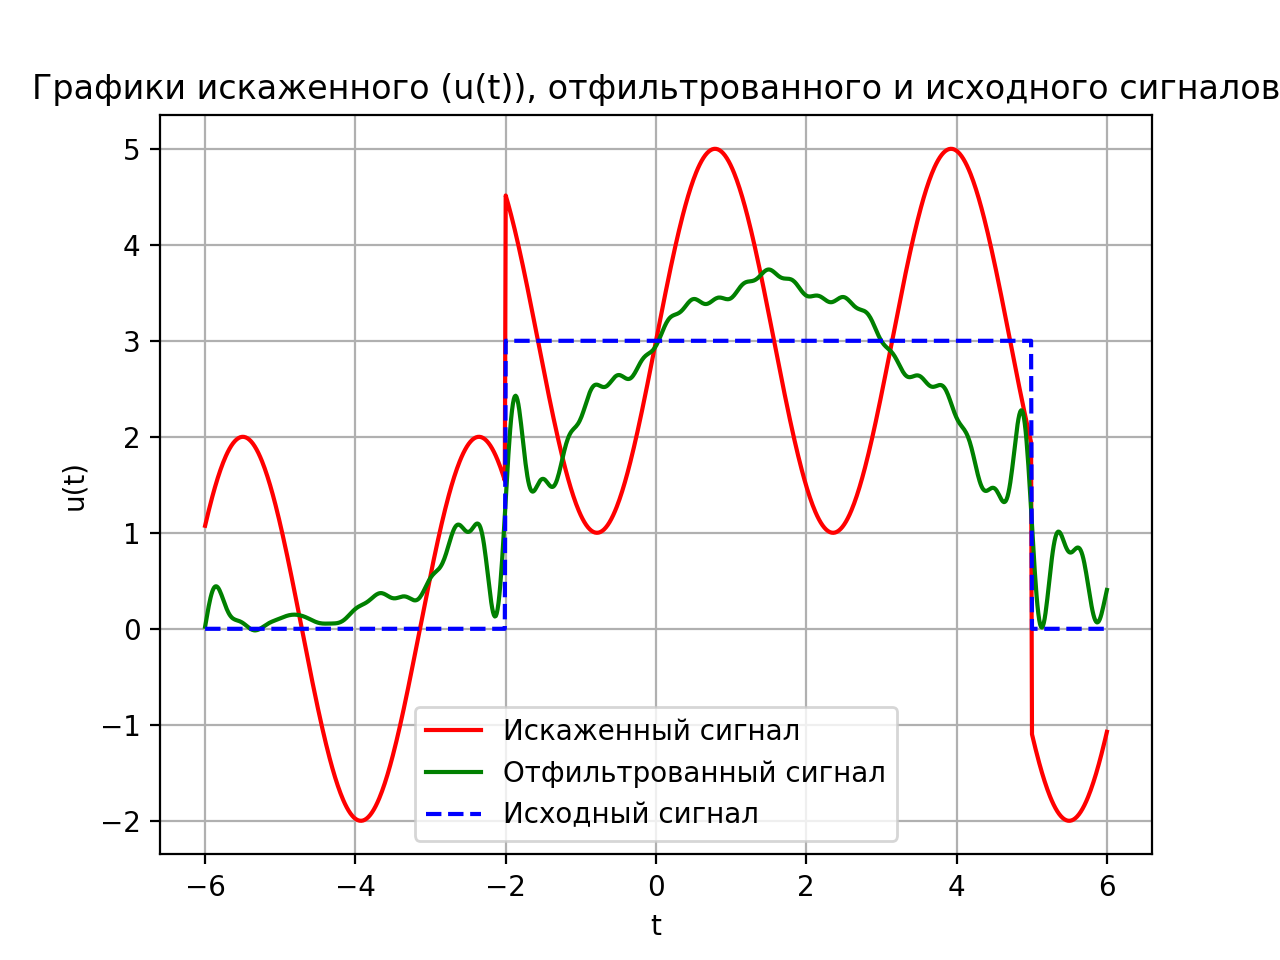
\includegraphics[scale=0.85]{media/1 task/specific_freq/Cleaned_0_2_2_-0,805:-0,156.png}
    \caption{Графики  $u(t)$, отфильтрованного и исходного сигналов при $b=0$,  $c=2$,  $d=2$}
    \label{fig:cleaned_0_2_2}
\end{figure}

\begin{figure}[ht!]
    \centering
    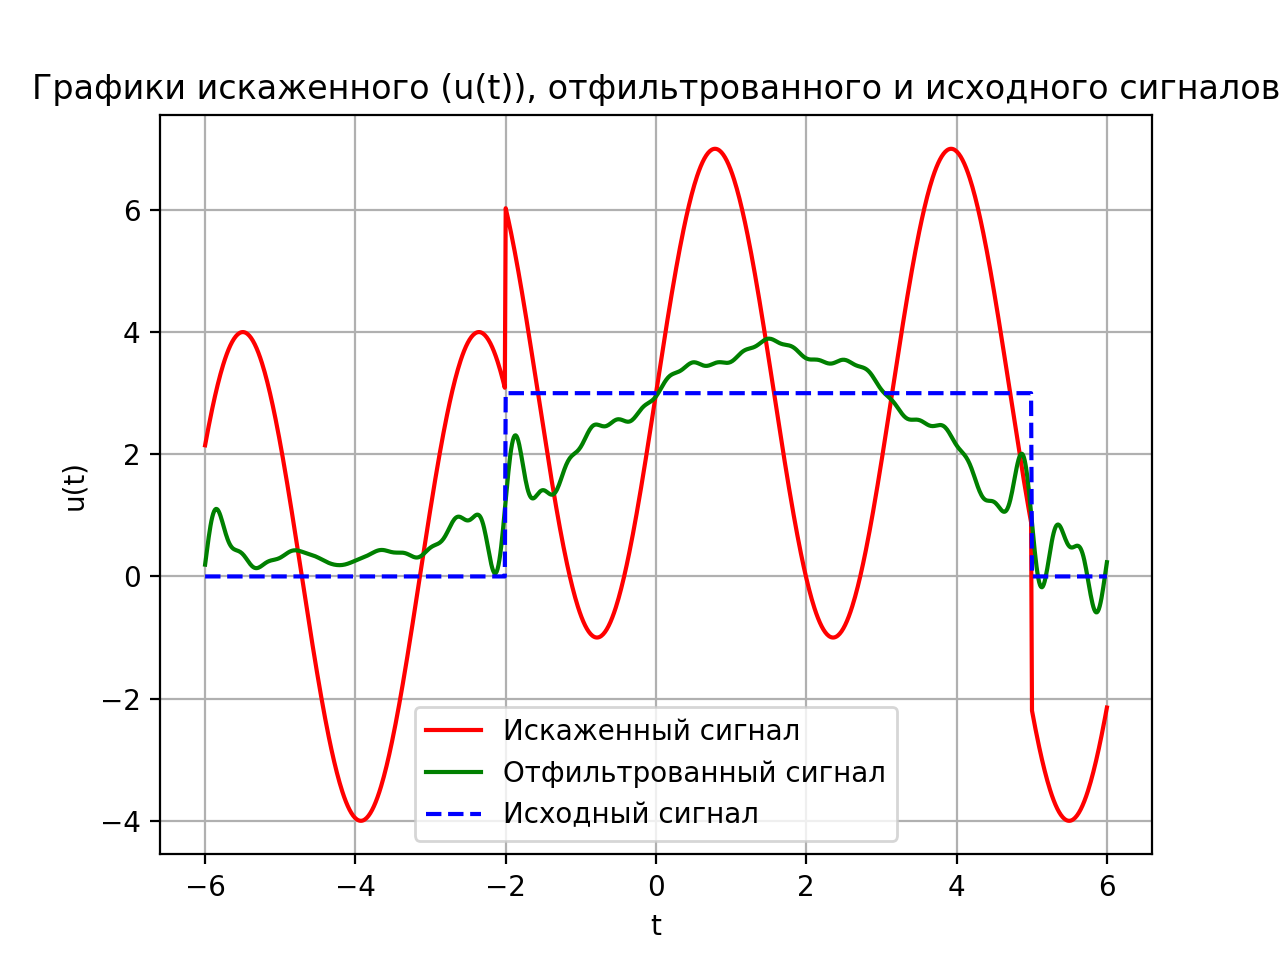
\includegraphics[scale=0.85]{media/1 task/specific_freq/Cleaned_0_4_2_-0,805:-0,156.png}
    \caption{Графики  $u(t)$, отфильтрованного и исходного сигналов при $b=0$,  $c=4$,  $d=2$}
    \label{fig:cleaned_0_4_2}
\end{figure}

\clearpage

\begin{figure}[ht!]
    \centering
    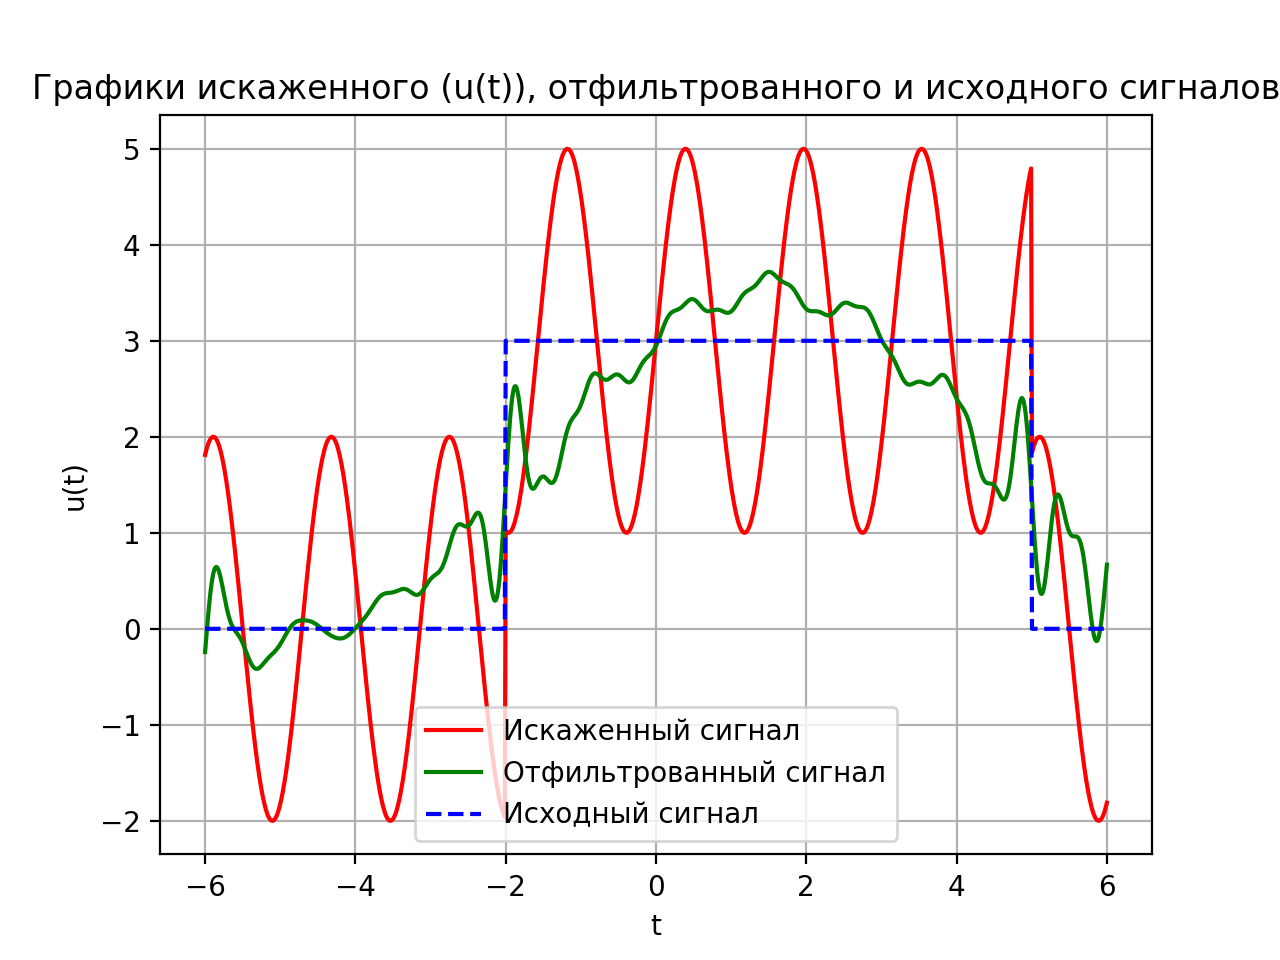
\includegraphics[scale=0.85]{media/1 task/specific_freq/Cleaned_0_2_4_-0,805:-0,156.png}
    \caption{Графики  $u(t)$, отфильтрованного и исходного сигналов при $b=0$,  $c=2$,  $d=4$}
    \label{fig:cleaned_0_2_4}
\end{figure}

Сравнение графиков подтверждает ранее сделанные нами выводы. Так как параметр $c$ оказывает влияние на амплитуду зашумленного сигнала, то у графика отфильтрованного сигнала также увеличиваются значения пиков. Параметр $d$, в свою очередь, оказывает влияние на частоту зашумленного и отфильтрованного сигналов, так что при увеличении значения этого параметра увеличивается частота отфильтрованного сигнала, и сигнал становится менее сглаженным.

\subsubsection{Влияние параметра $b$}\label{b_ex}

Теперь рассмотрим влияние параметра $b$ на фильтрацию. Зафиксируем параметры $c=4, d=2$ и частоты  $\nu_0 \in [0.153, 0.8]$

\begin{figure}[ht!]
    \centering
    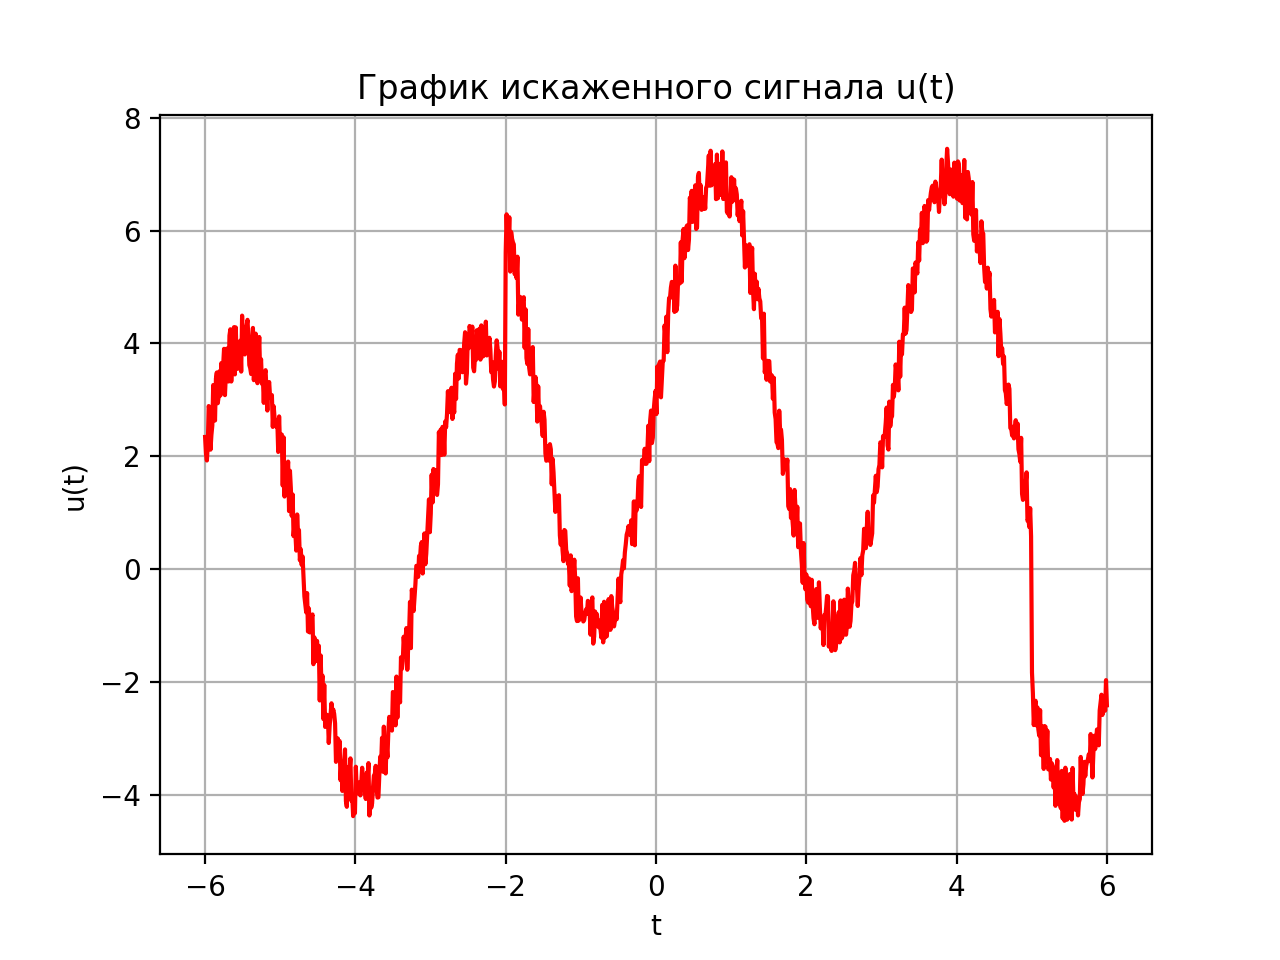
\includegraphics[scale=0.75]{media/1 task/specific_freq/Noisy_1_4_2.png}
    \caption{График функции $u(t)$ при $b=1$,  $c=4$,  $d=2$}
    \label{fig:noisy_1_4_2}
\end{figure}

\begin{figure}[ht!]
    \centering
    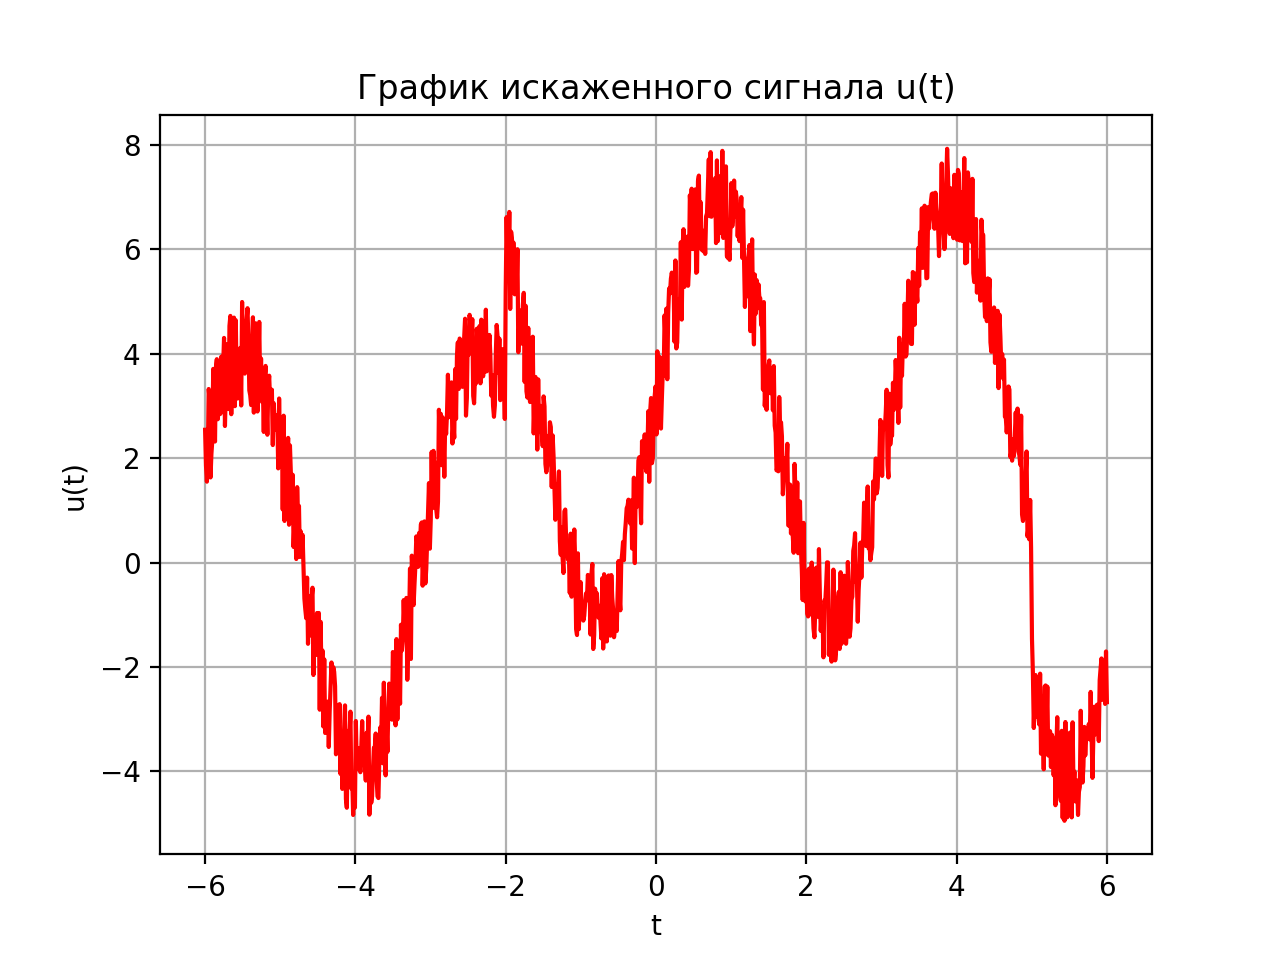
\includegraphics[scale=0.75]{media/1 task/specific_freq/Noisy_2_4_2.png}
    \caption{График функции $u(t)$ при $b=2$,  $c=4$,  $d=2$}
    \label{fig:noisy_2_4_2}
\end{figure}

\clearpage

\begin{figure}[ht!]
    \centering
    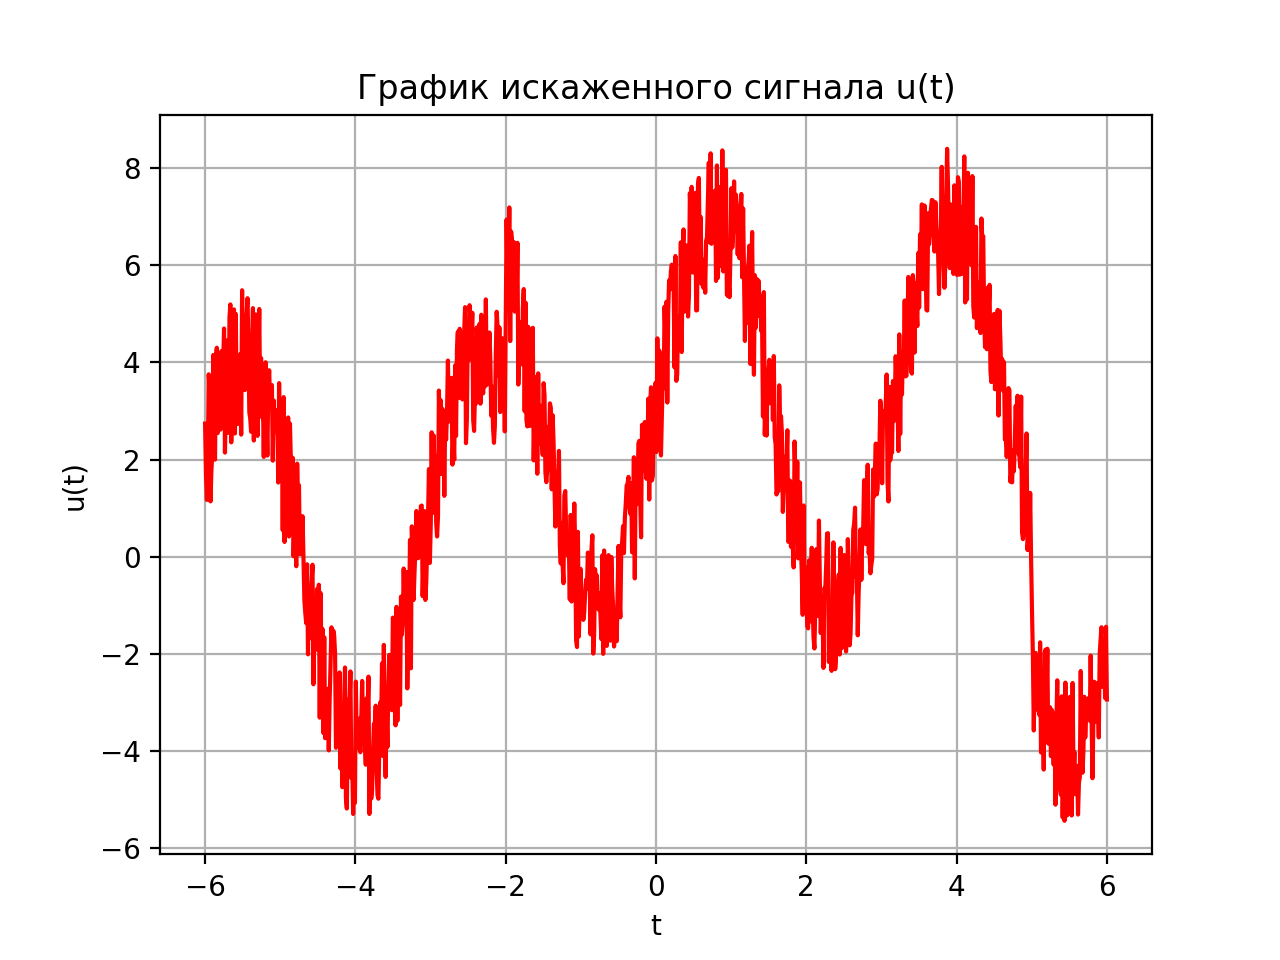
\includegraphics[scale=0.75]{media/1 task/specific_freq/Noisy_3_4_2.png}
    \caption{График функции $u(t)$ при $b=3$,  $c=4$,  $d=2$}
    \label{fig:noisy_3_4_2}
\end{figure}

Графики подтверждают вывод, сделанный в пункте \ref{high_freq}, о влиянии параметра $b$ на хаотический шум в зашумленном сигнале. А мы идём дальше к Фурье-образам!

\clearpage

\begin{figure}[ht!]
    \centering
    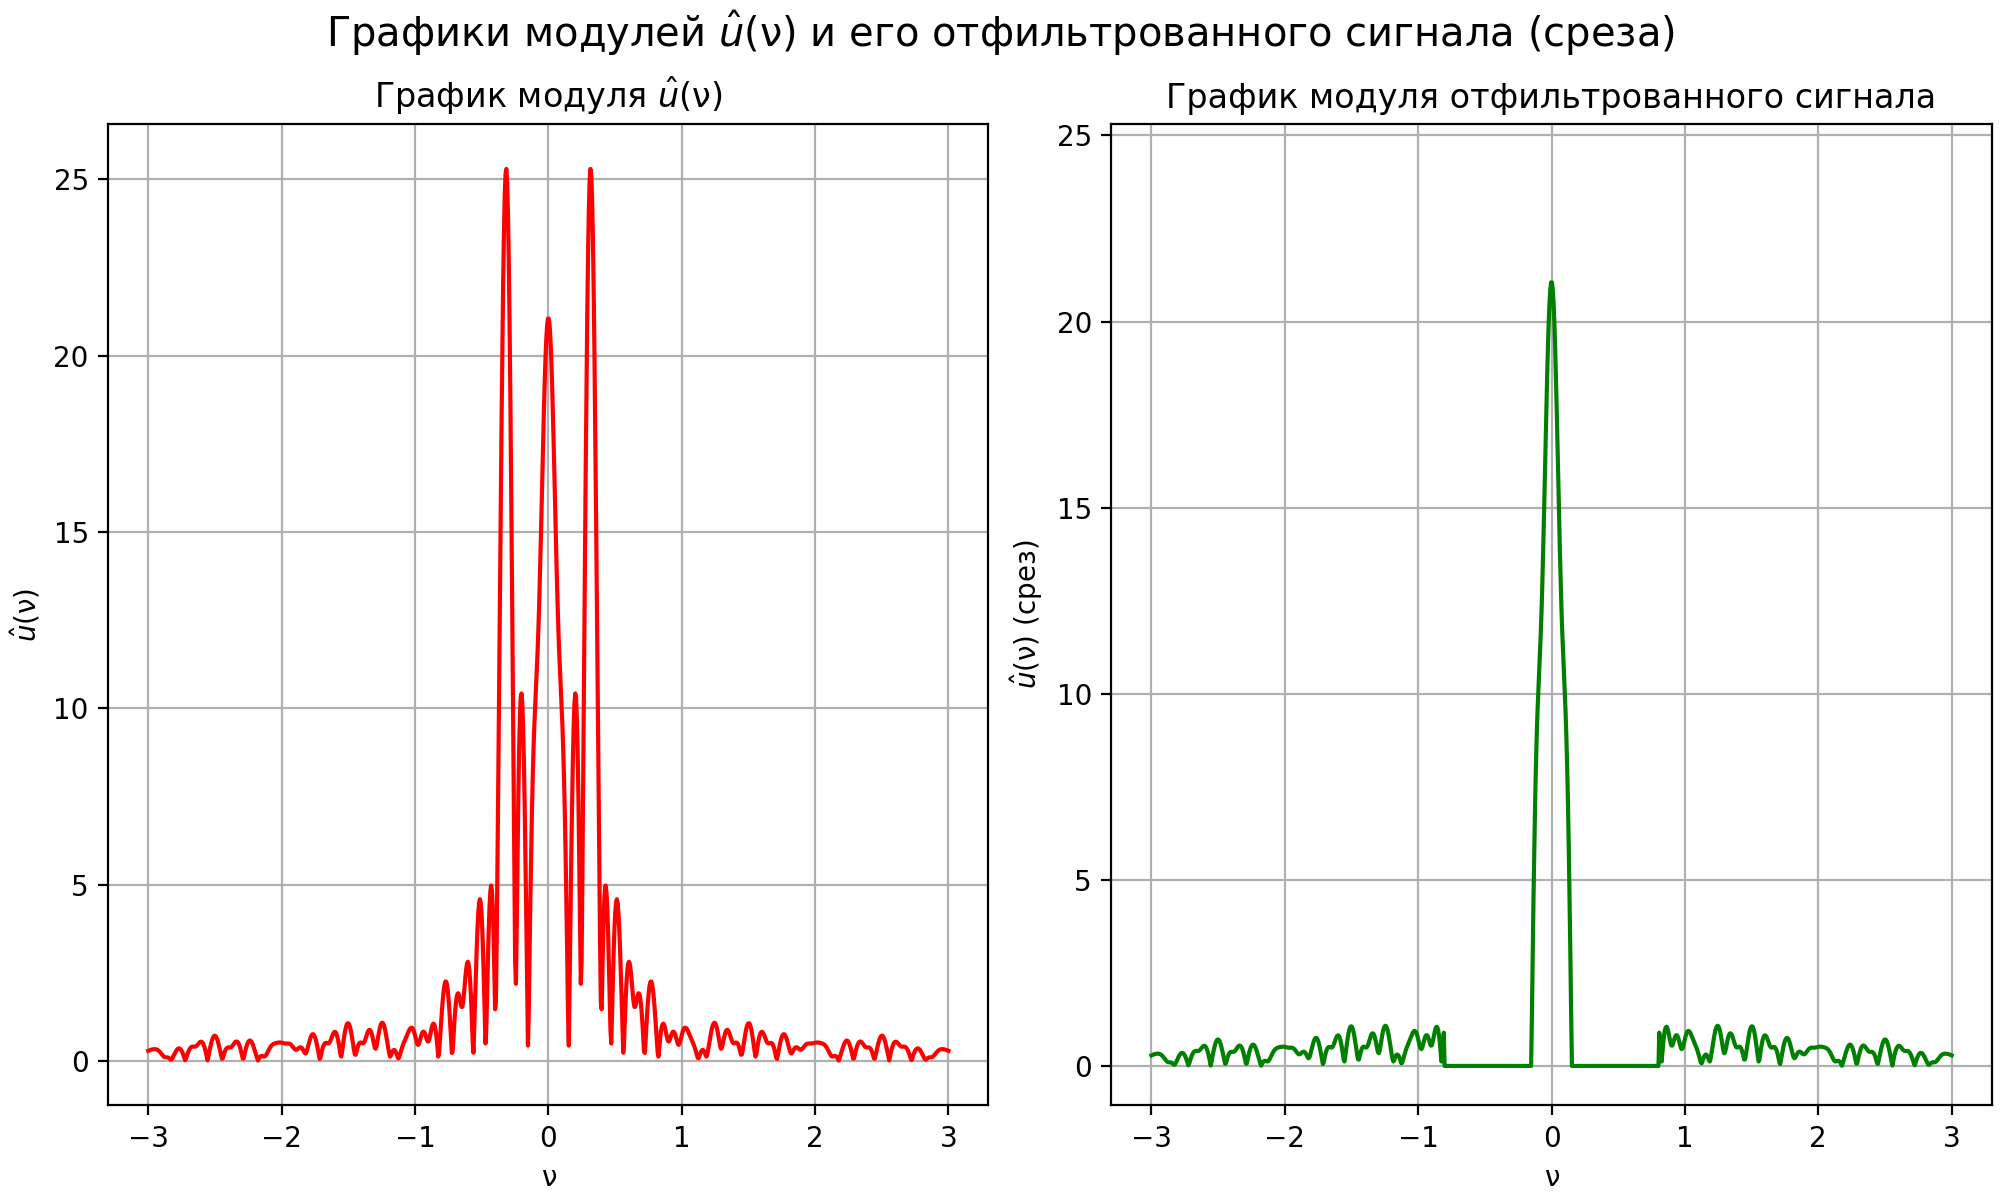
\includegraphics[scale=0.55]{media/1 task/specific_freq/Fourier_Image_1_4_2_-0,8:-0,153.png}
    \caption{Графики модулей Фурье-образа $u(t)$ и отфильтрованного сигнала при $b=1$,  $c=4$,  $d=2$}
    \label{fig:four_1_4_2}
\end{figure}


\begin{figure}[ht!]
    \centering
    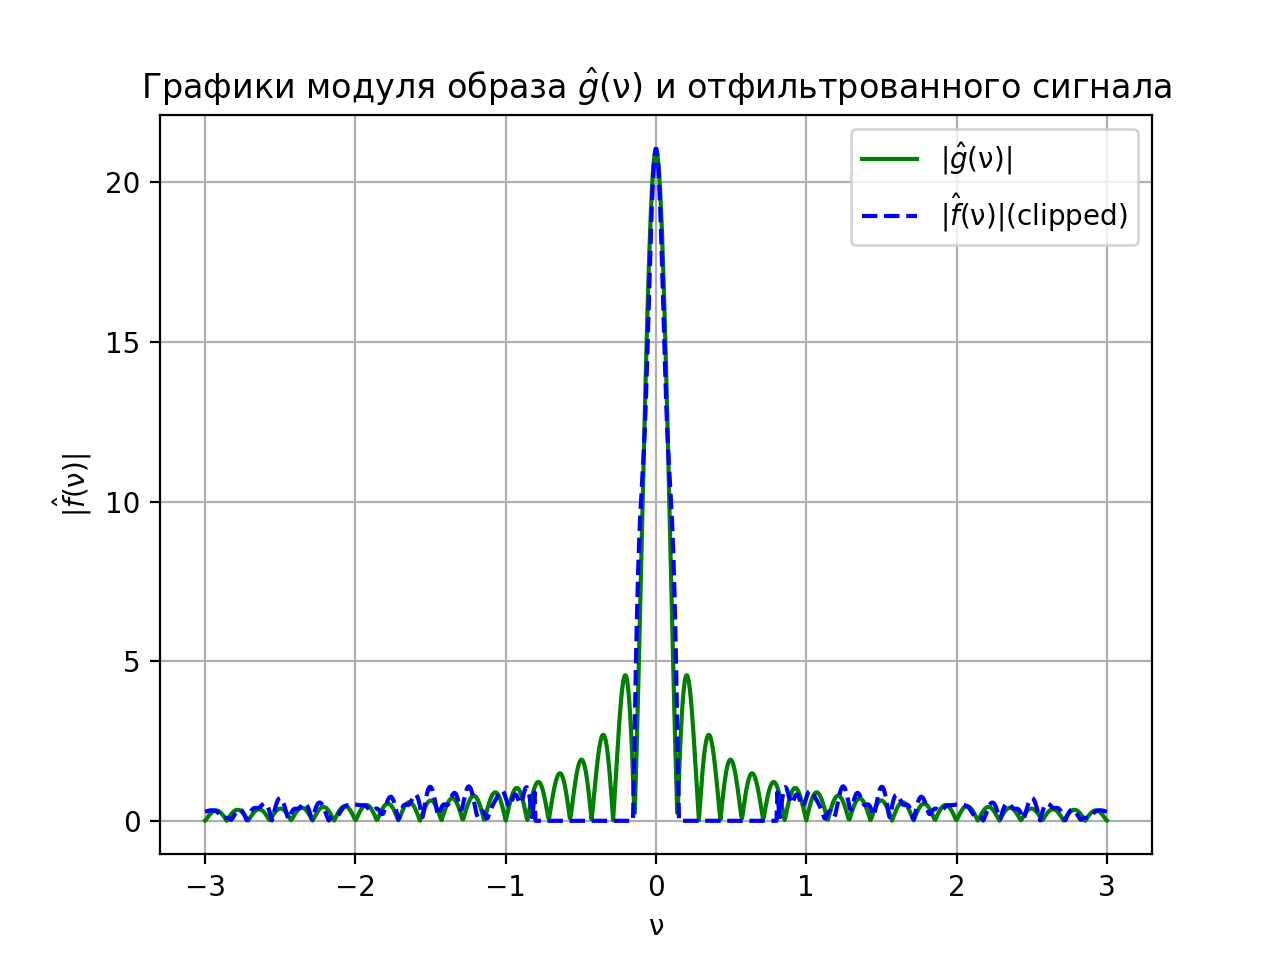
\includegraphics[scale=0.55]{media/1 task/specific_freq/Fourier_Image_Comparison_1_4_2_-0,8:-0,153.png}
    \caption{Сравнительные графики модулей Фурье-образа $g(t)$ и отфильтрованного сигнала при $b=1$,  $c=4$,  $d=2$}
    \label{fig:fourc_1_4_2}
\end{figure}

\begin{figure}[ht!]
    \centering
    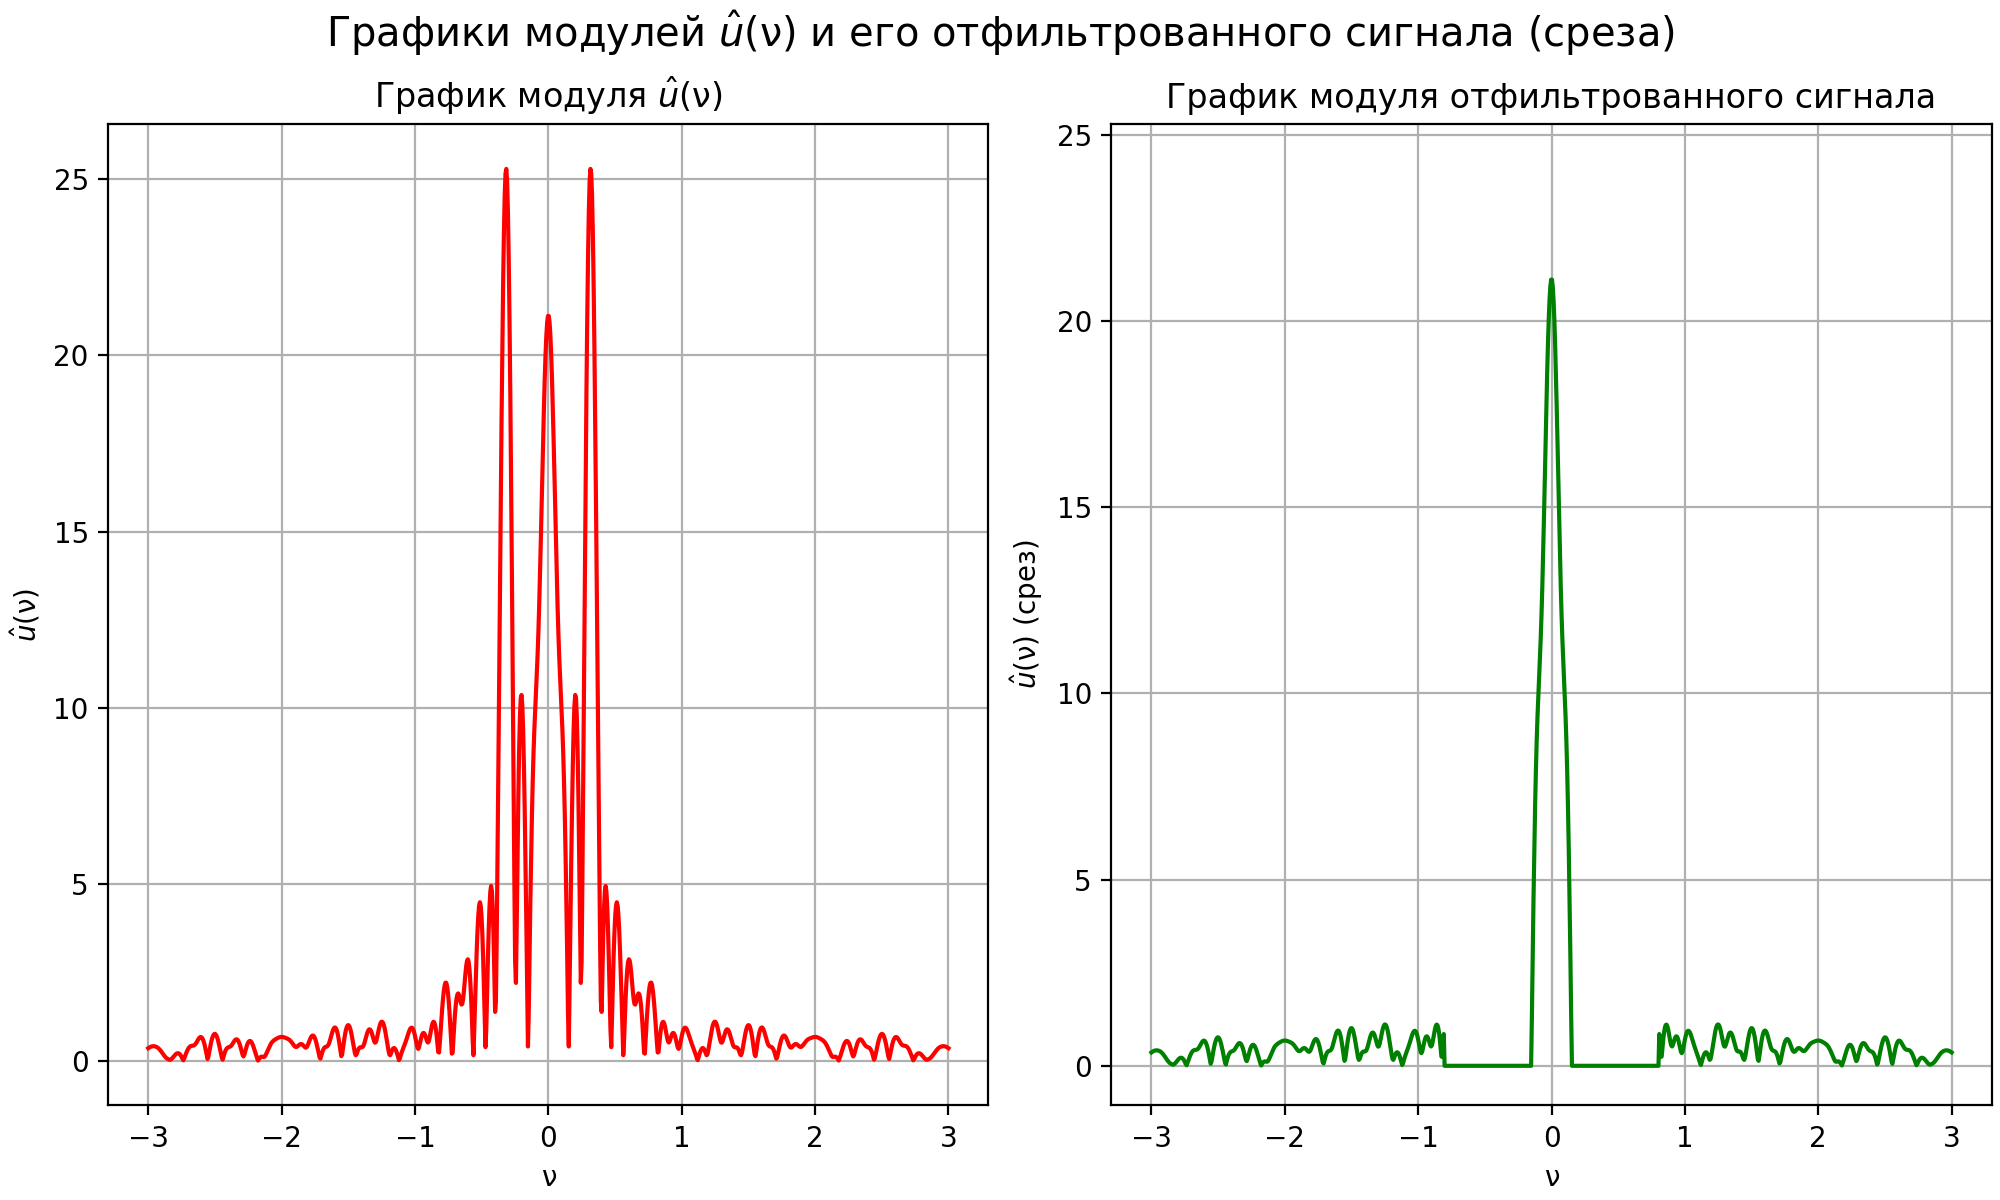
\includegraphics[scale=0.55]{media/1 task/specific_freq/Fourier_Image_2_4_2_-0,8:-0,153.png}
    \caption{Графики модулей Фурье-образа $u(t)$ и отфильтрованного сигнала при $b=2$,  $c=4$,  $d=2$}
    \label{fig:four_2_4_2}
\end{figure}

На графиках можно чётко проследить влияние параметра $b$ на Фурье-образ. При увеличении значения параметра мы видим, что значение модуля при некоторых частотах возрастает, при других --- уменьшается. В сравнении с графиками из пункта \ref{b_0} заметно появление хаотического шума.

\begin{figure}[ht!]
    \centering
    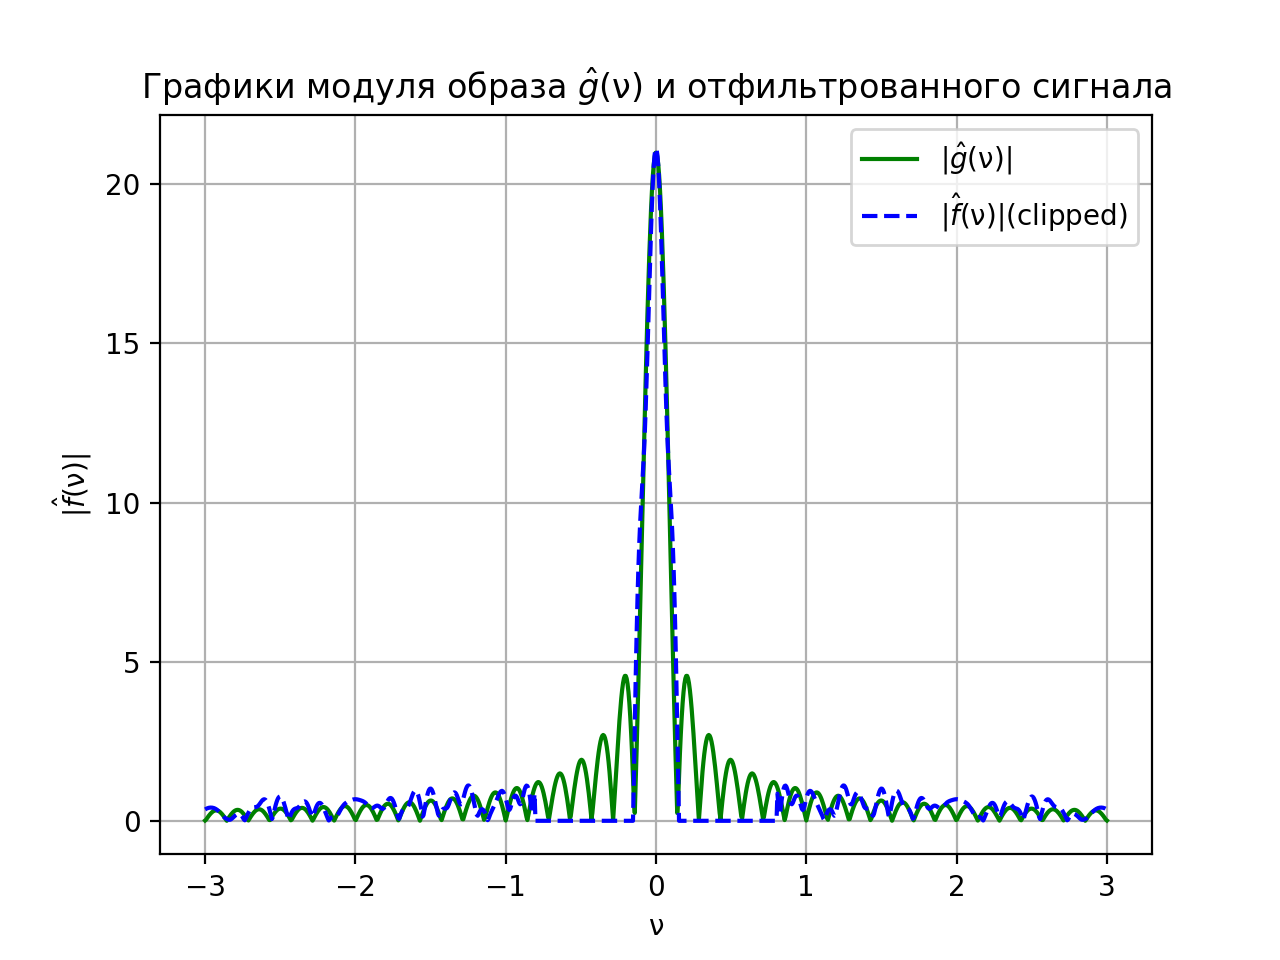
\includegraphics[scale=0.55]{media/1 task/specific_freq/Fourier_Image_Comparison_2_4_2_-0,8:-0,153.png}
    \caption{Сравнительные графики модулей Фурье-образа $g(t)$ и отфильтрованного сигнала при $b=2$,  $c=4$,  $d=2$}
    \label{fig:fourc_2_4_2}
\end{figure}



\begin{figure}[ht!]
    \centering
    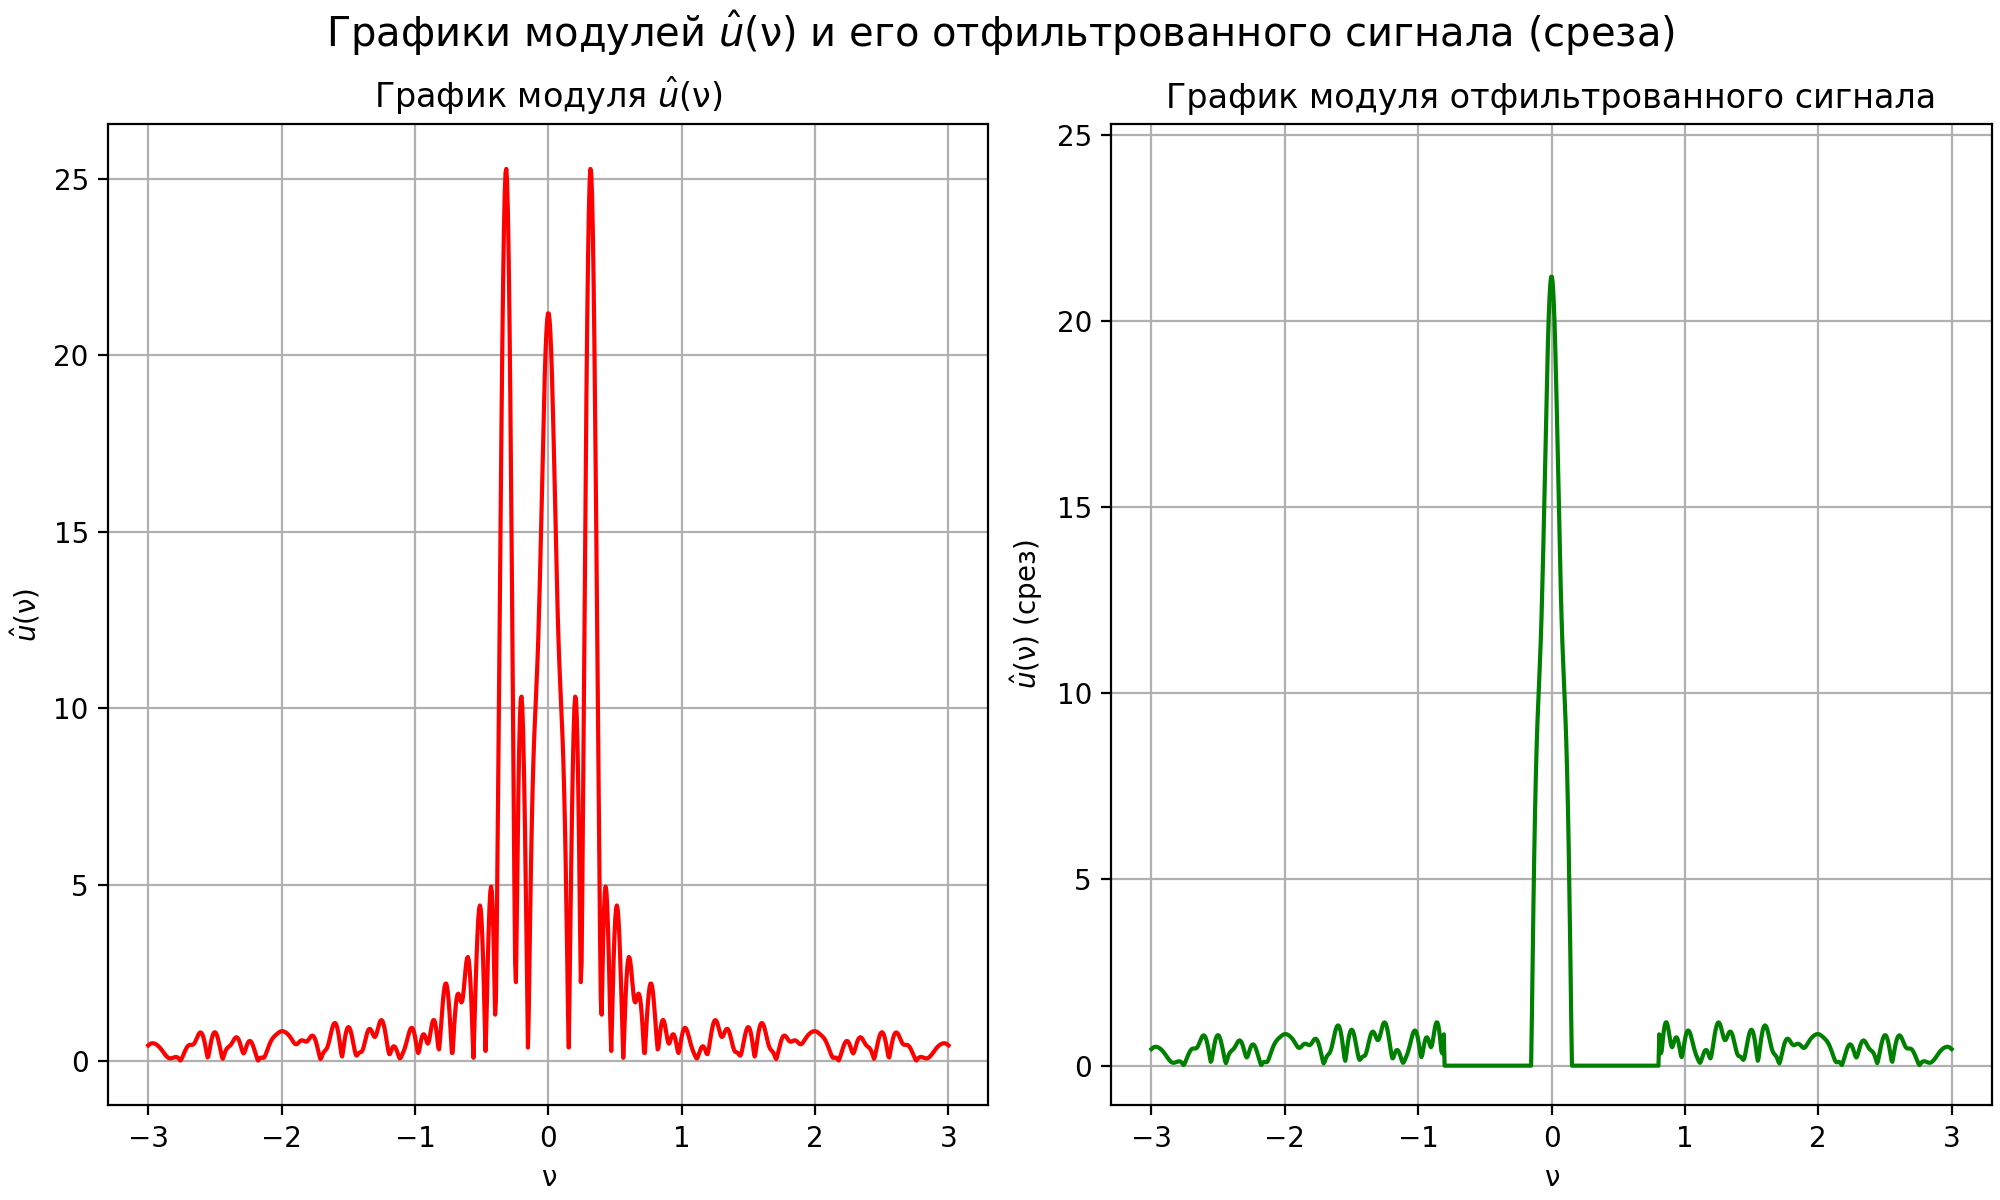
\includegraphics[scale=0.55]{media/1 task/specific_freq/Fourier_Image_3_4_2_-0,8:-0,153.png}
    \caption{Графики модулей Фурье-образа $f(t)$ и отфильтрованного сигнала при $b=3$,  $c=4$,  $d=2$}
    \label{fig:four_3_4_2}
\end{figure}

\begin{figure}[ht!]
    \centering
    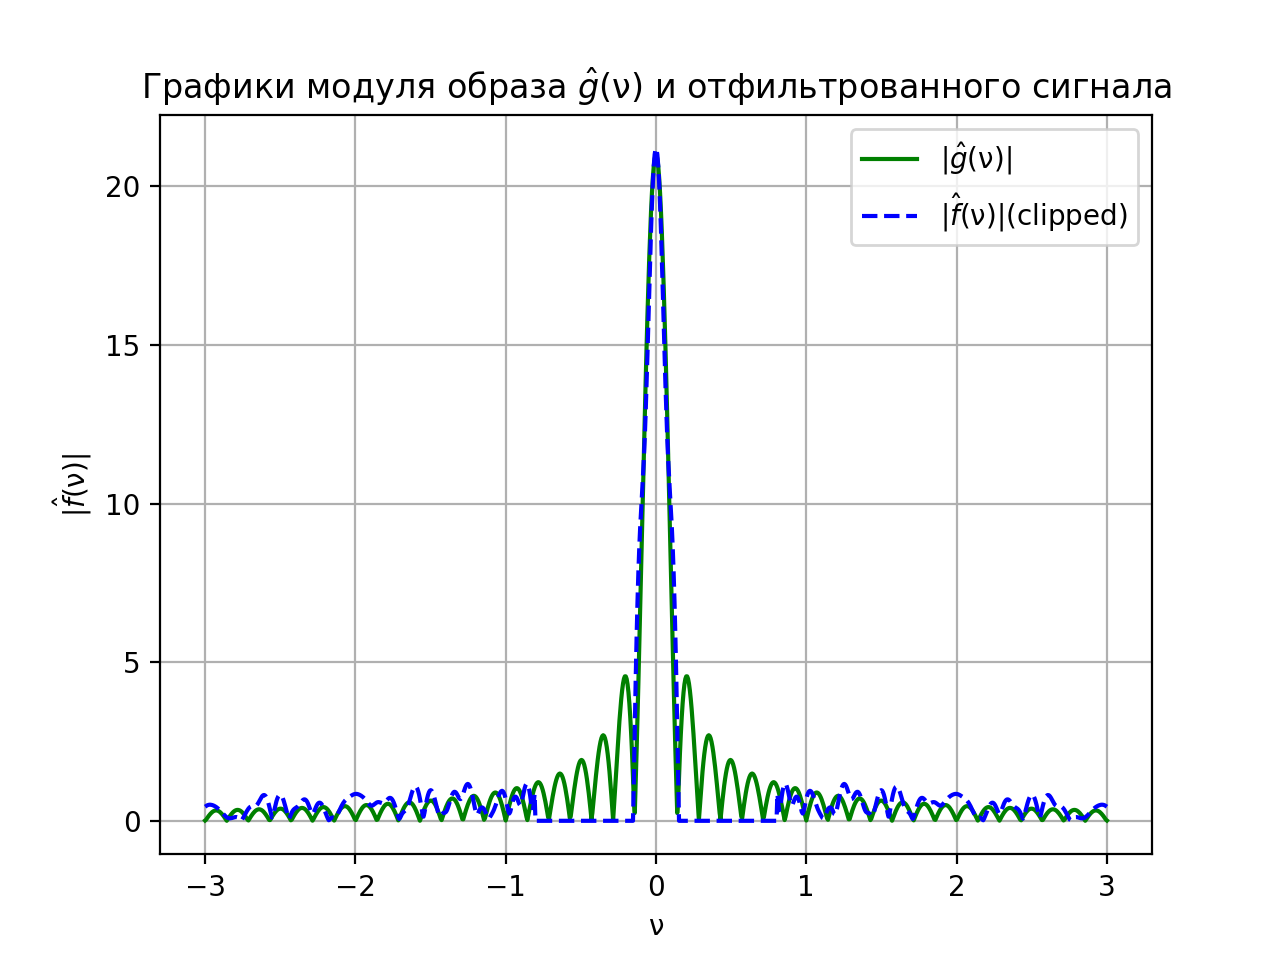
\includegraphics[scale=0.55]{media/1 task/specific_freq/Fourier_Image_Comparison_3_4_2_-0,8:-0,153.png}
    \caption{Сравнительные графики модулей Фурье-образа $g(t)$ и отфильтрованного сигнала при  $b=3$,  $c=4$,  $d=2$}
    \label{fig:fourc_3_4_2}
\end{figure}

\clearpage

\begin{figure}[ht!]
    \centering
    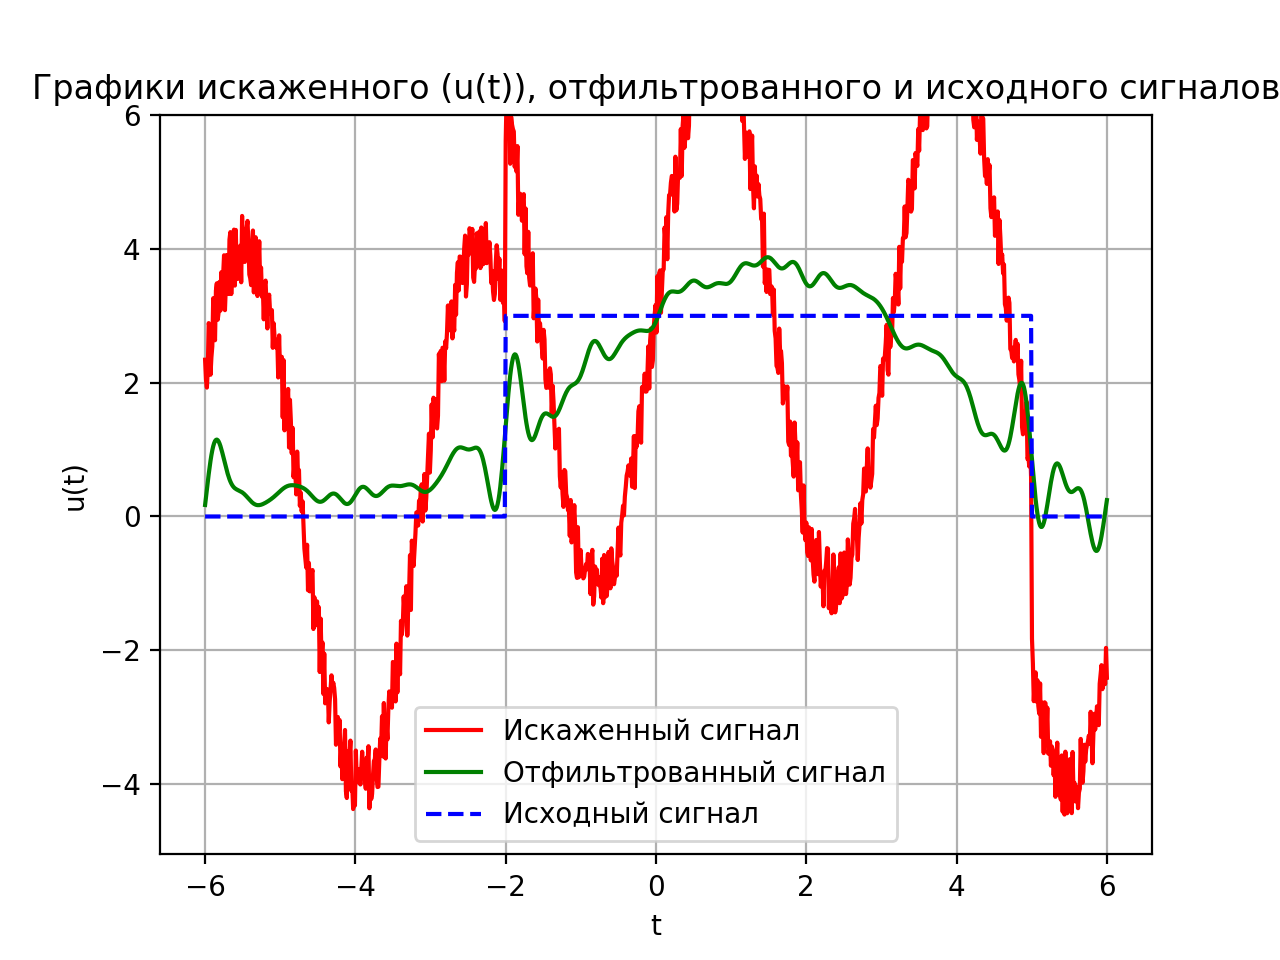
\includegraphics[scale=0.85]{media/1 task/specific_freq/Cleaned_1_4_2_-0,8:-0,153.png}
    \caption{Графики  $u(t)$, отфильтрованного и исходного сигналов при $b=1$,  $c=4$,  $d=2$}
    \label{fig:cleaned_1_4_2}
\end{figure}

\begin{figure}[ht!]
    \centering
    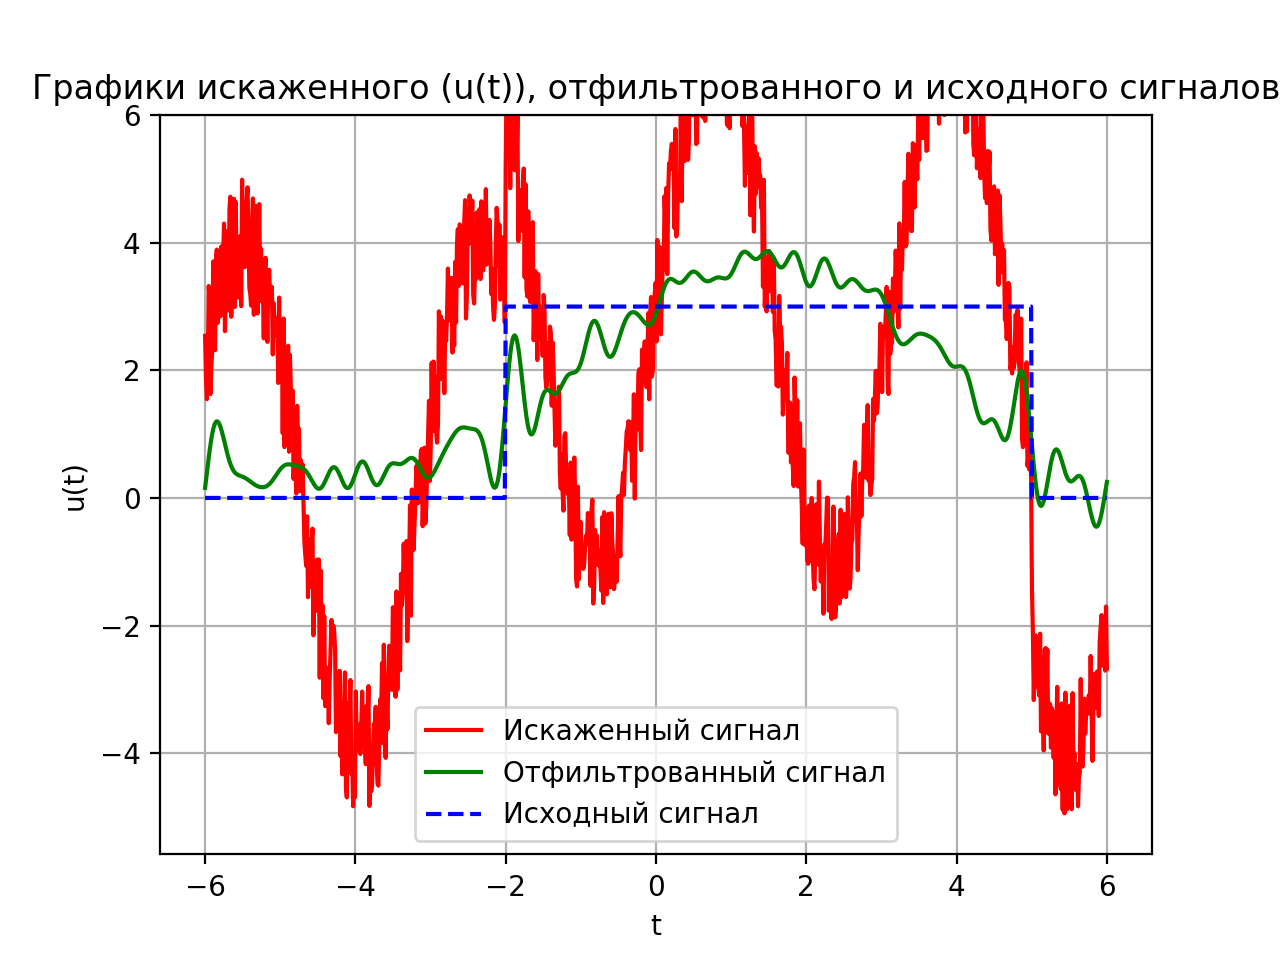
\includegraphics[scale=0.85]{media/1 task/specific_freq/Cleaned_2_4_2_-0,8:-0,153.png}
    \caption{Графики  $u(t)$, отфильтрованного и исходного сигналов при $b=2$,  $c=4$,  $d=2$}
    \label{fig:cleaned_2_4_2}
\end{figure}

\clearpage

\begin{figure}[ht!]
    \centering
    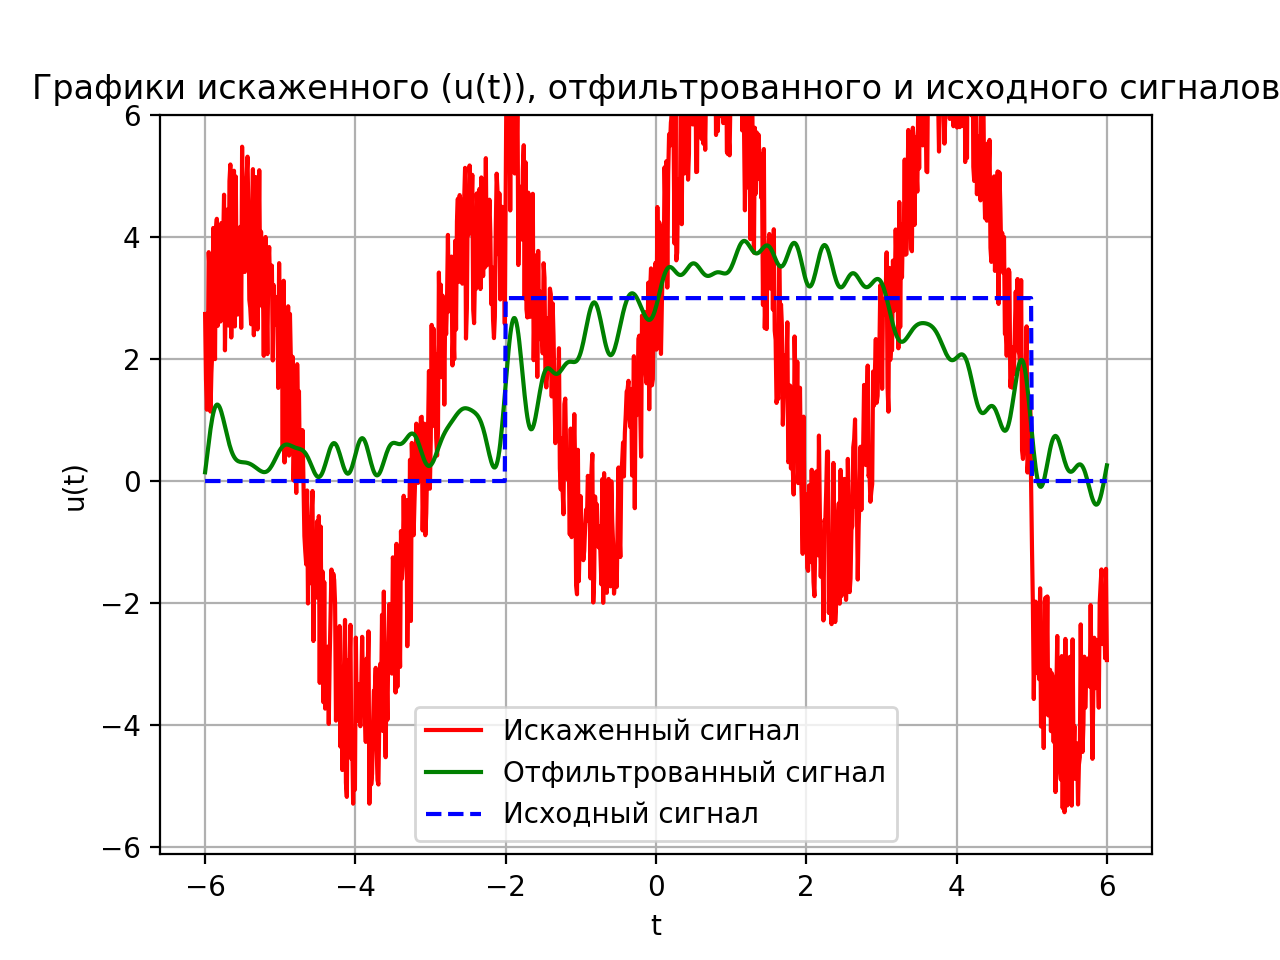
\includegraphics[scale=0.85]{media/1 task/specific_freq/Cleaned_3_4_2_-0,8:-0,153.png}
    \caption{Графики  $u(t)$, отфильтрованного и исходного сигналов при $b=3$,  $c=4$,  $d=2$}
    \label{fig:cleaned_3_4_2}
\end{figure}

При увеличении $b$, как говорилось ранее, увеличивается влияние хаотического шума, поэтому при одинаковом фильтрационном интервале отфильтрованный Фурье-образ начинает удаляться по норме от образа исходного сигнала (см. рисунки \ref{fig:fourc_1_4_2}, \ref{fig:fourc_2_4_2}, \ref{fig:fourc_3_4_2}). Это приводит к тому, что у отфильтрованного сигнала увеличиваются значения пиков при одном и том же значении $t$.

\subsubsection{Подбираем правильные частоты среза }

Возьмём сигнал с параметрами $b=2, c=4, d=2$ из прошлого пункта \ref{b_ex}. График сигнала представлен на рисунке \ref{fig:noisy_2_4_2}. Нами уже был рассмотрен промежуток $\nu_0 \in [0.153, 0.8]$. Теперь попробуем подобрать частоты таким образом, чтобы максимально приблизить его к исходному сигналу $g(t)$.

\clearpage

\begin{figure}[ht!]
    \centering
    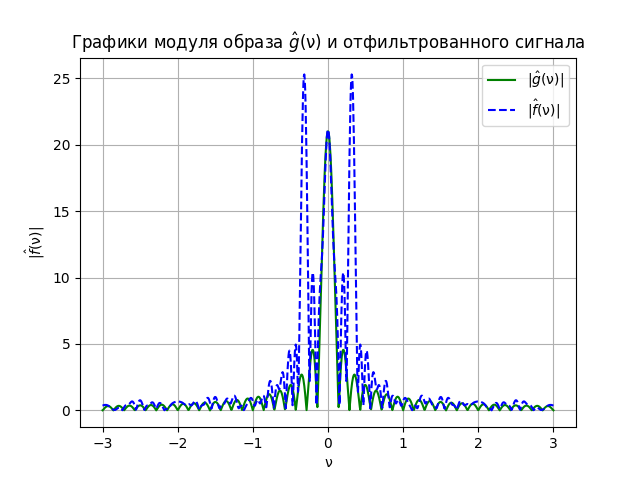
\includegraphics[scale=0.65]{media/1 task/specific_freq/Image_2_4_2_Begi.png}
    \caption{Сравнительные графики модулей Фурье-образа $g(t)$ и сигнала при  $b=2$,  $c=4$,  $d=2$}
    \label{fig:fourcorig_2_4_2}
\end{figure}

Для начала попробуем более точечнее отфильтровать частоты из уже использованного диапазона. Интервалы частот, которые мы отбросим:

\begin{center}
    $\nu_0 \in [0.153, 0.65] \cup [0.72, 0.8044]$
\end{center}

\begin{figure}[ht!]
    \centering
    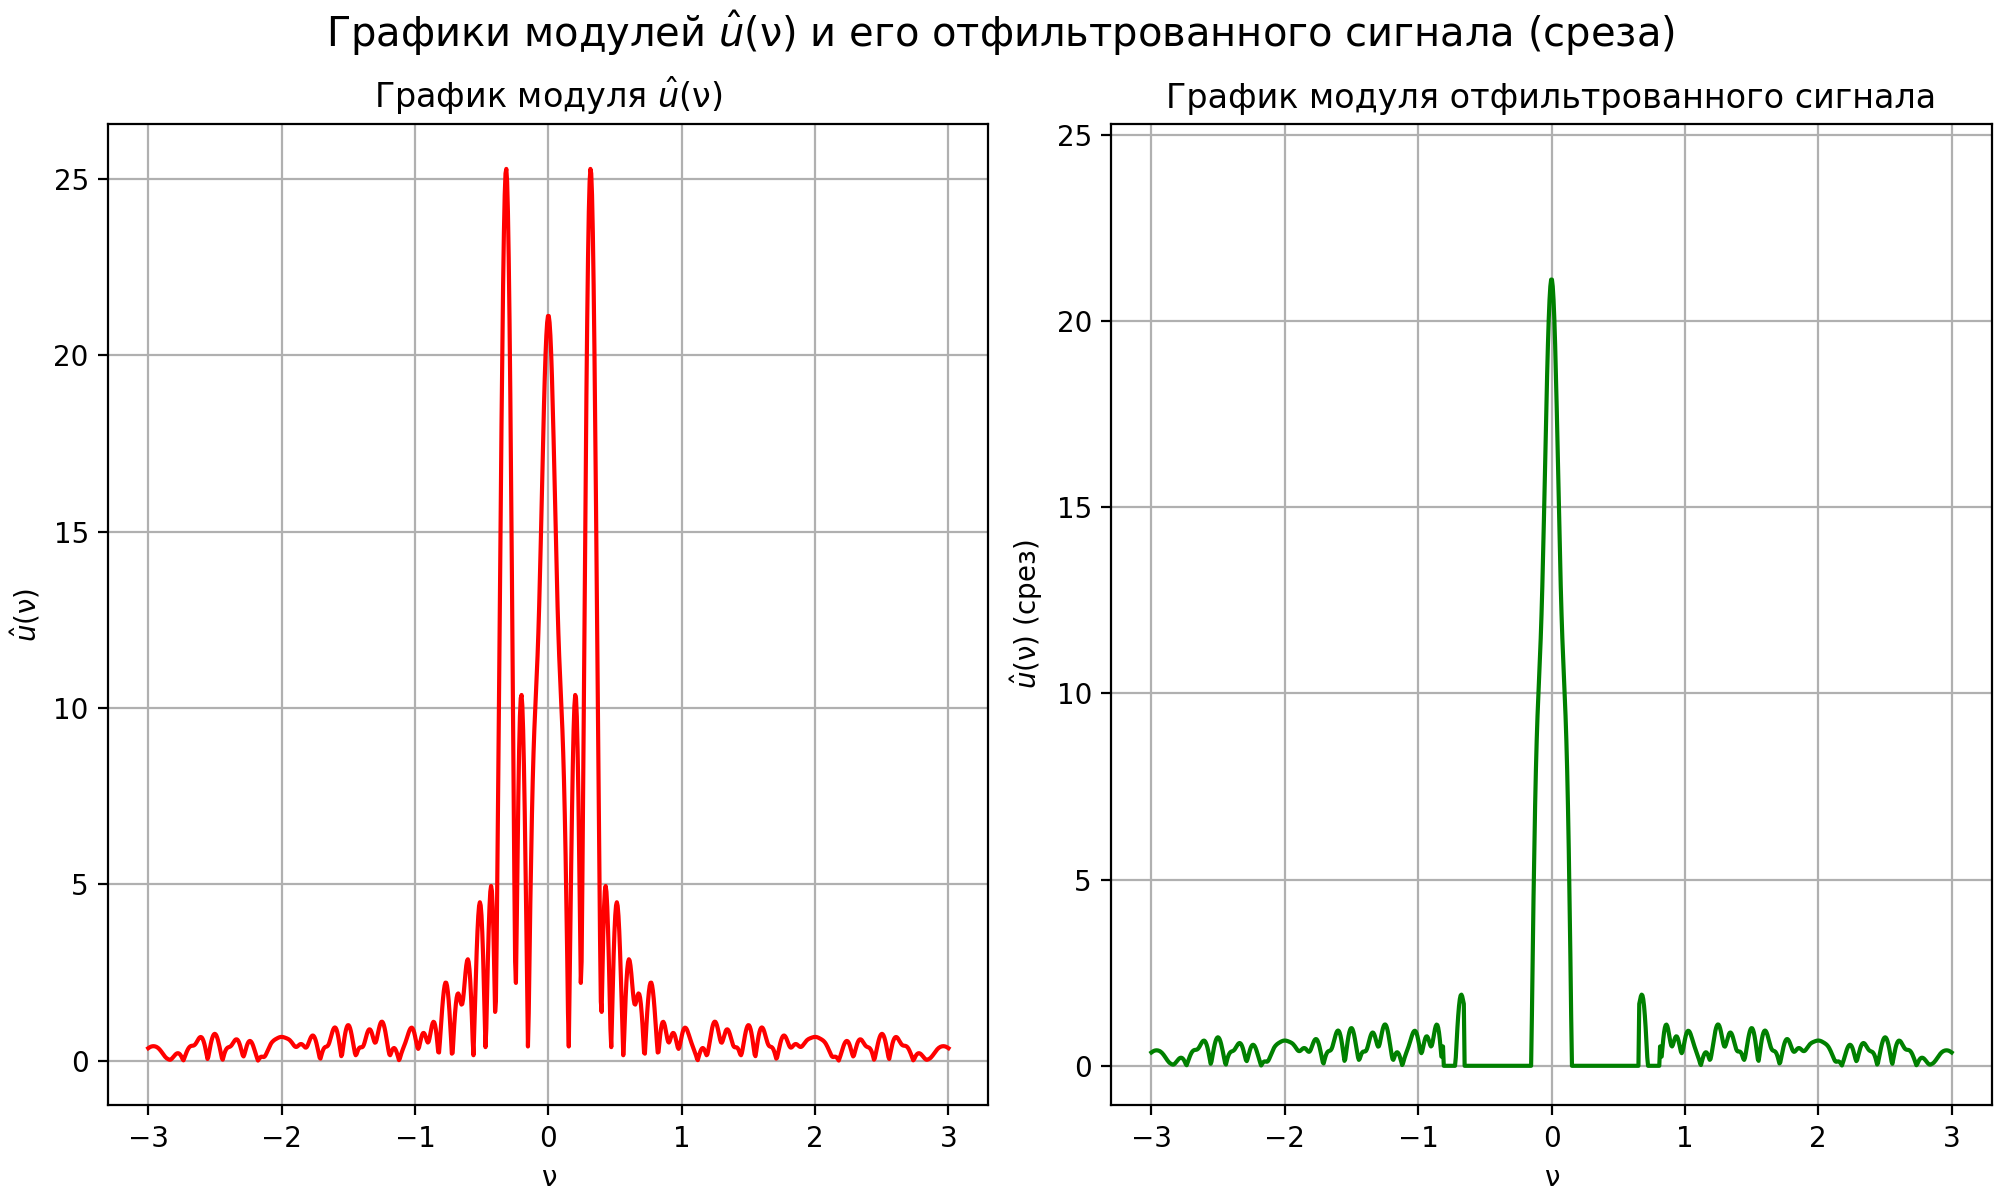
\includegraphics[scale=0.55]{media/1 task/specific_freq/Fourier_Image_2_4_2_-0,65:-0,153_-0,8044:-0,72.png}
    \caption{Графики модулей Фурье-образа $u(t)$ и отфильтрованного сигнала при $b=2$,  $c=4$,  $d=2$}
    \label{fig:four_2_4_2_2intervals}
\end{figure}

\begin{figure}[ht!]
    \centering
    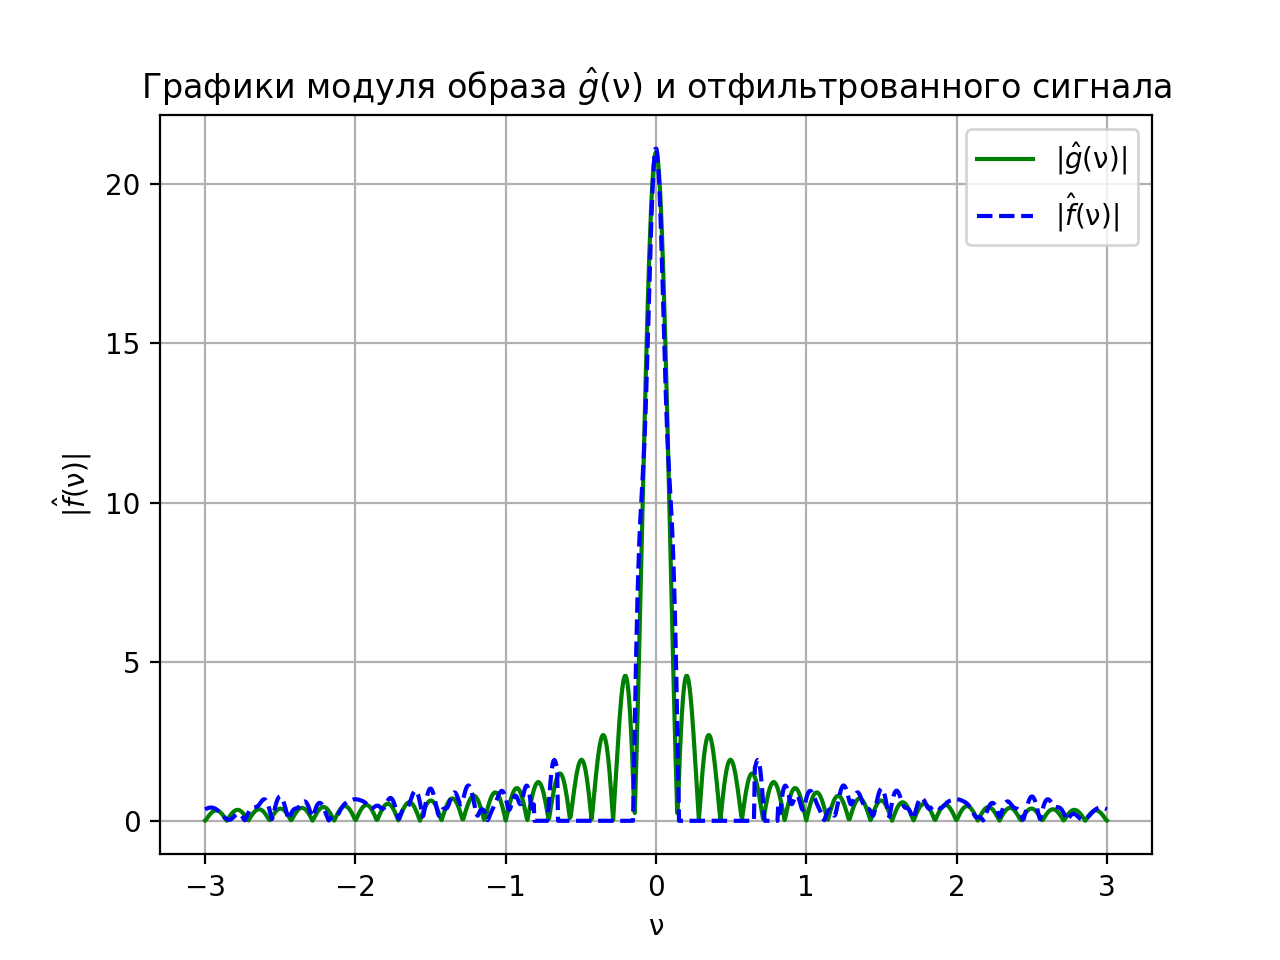
\includegraphics[scale=0.55]{media/1 task/specific_freq/Fourier_Image_Comparison_2_4_2_-0,65:-0,153_-0,8044:-0,72.png}
    \caption{Сравнительные графики модулей Фурье-образа $g(t)$ и отфильтрованного сигнала при $b=2$,  $c=4$,  $d=2$}
    \label{fig:fourc_2_4_2_2intervlas}
\end{figure}

\begin{figure}[ht!]
    \centering
    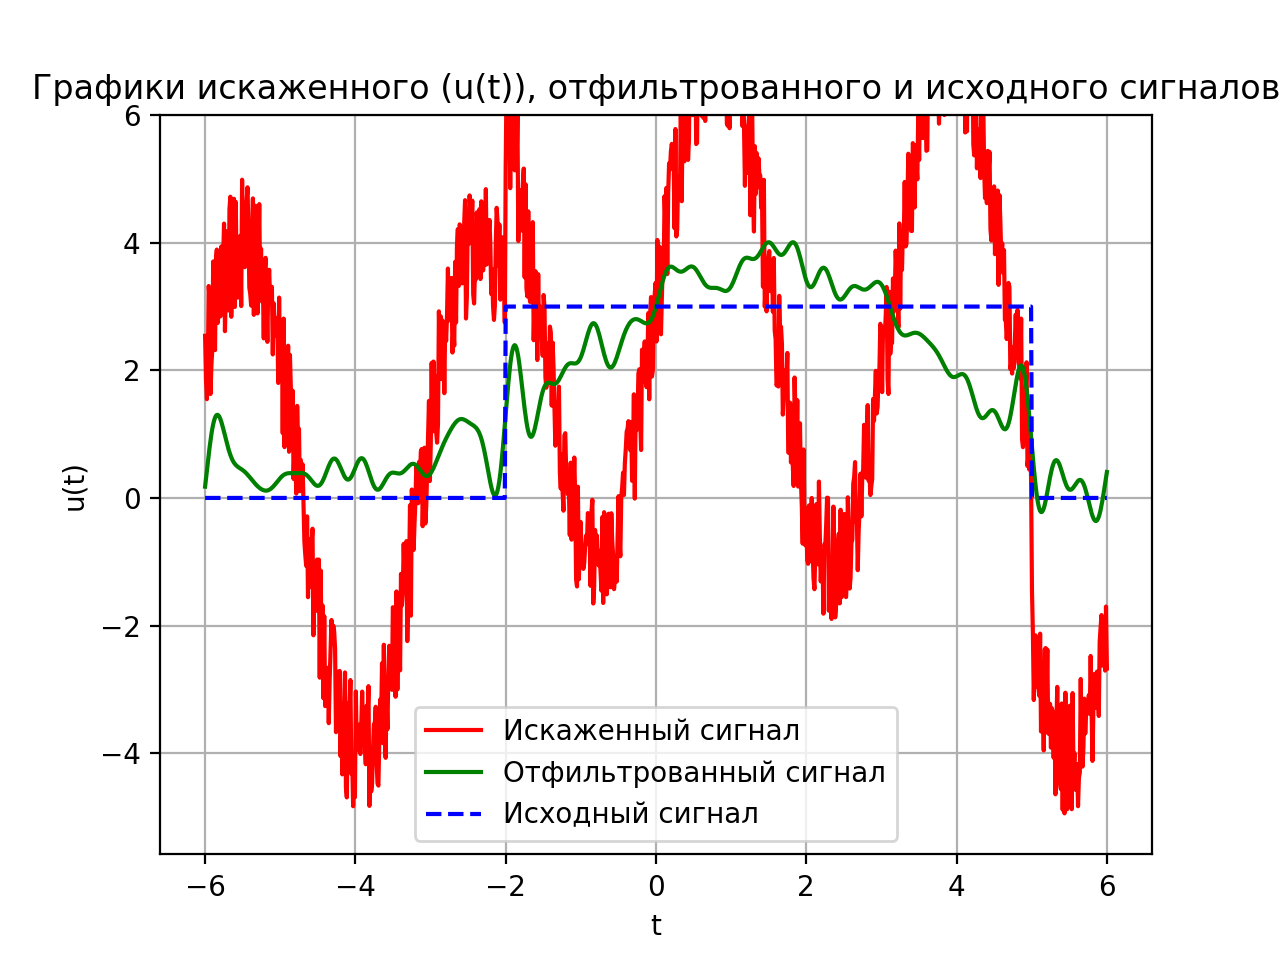
\includegraphics[scale=0.65]{media/1 task/specific_freq/Cleaned_2_4_2_-0,65:-0,153_-0,8044:-0,72.png}
    \caption{Графики  $u(t)$, отфильтрованного и исходного сигналов при $b=2$,  $c=4$,  $d=2$}
    \label{fig:cleaned_2_4_2_2intervals}
\end{figure}

Теперь попробуем дополнительно отбросить некоторые высокие частоты. Тогда интервал частот, которые мы отбросим, будут выглядеть следующим образом:

\begin{center}
    $\nu_0 \in [0.153, 0.65] \cup [0.72, 0.8044] \cup [1.21, 1.3] \cup [1.922, 2.07] \cup [2.47, 2.67]$
\end{center}

\begin{figure}[ht!]
    \centering
    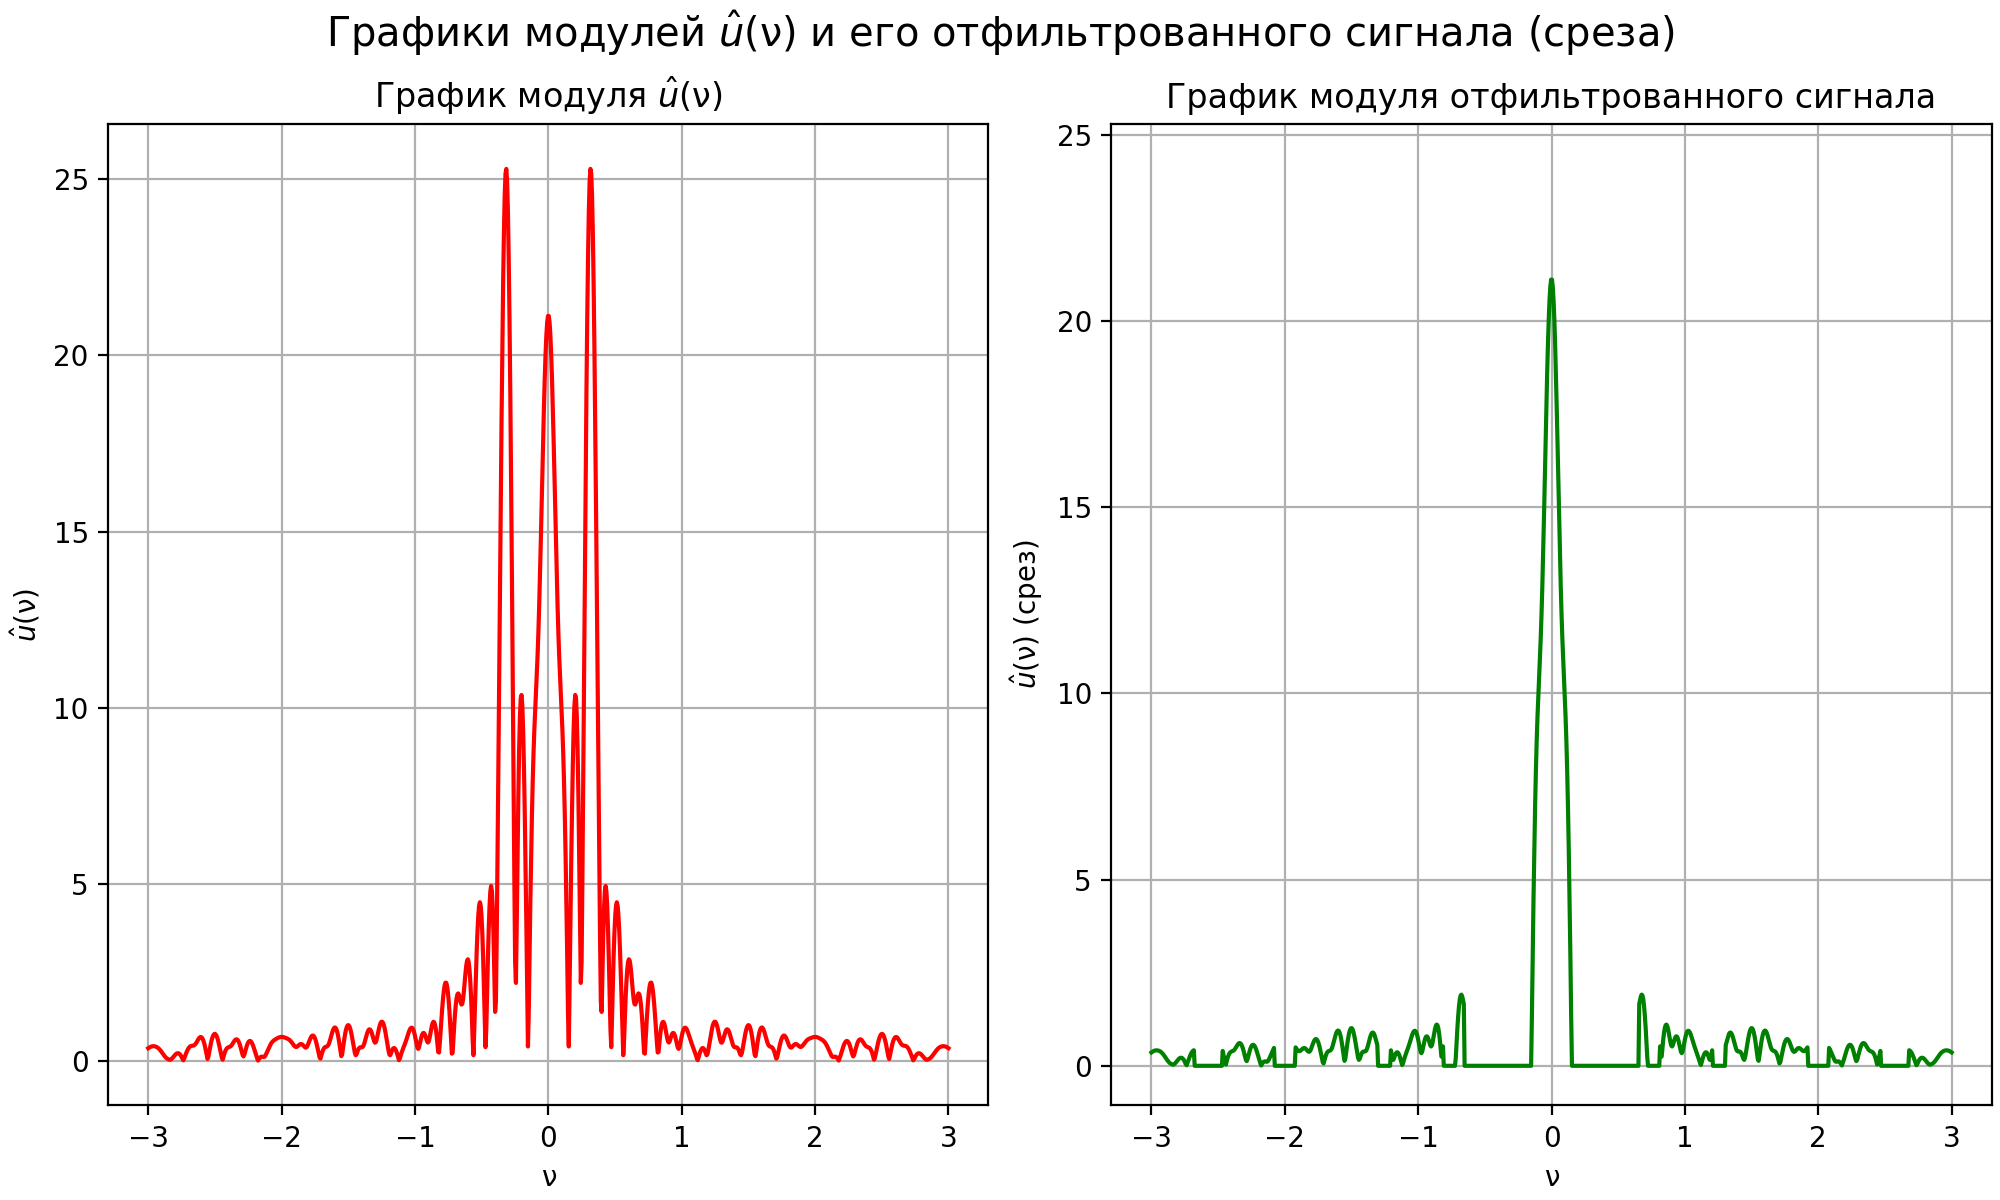
\includegraphics[scale=0.55]{media/1 task/specific_freq/Fourier_Image_2_4_2_-0,65:-0,153_-0,8044:-0,72_-1,3:-1,21_-2,07:-1,922_-2,67:-2,47.png}
    \caption{Графики модулей Фурье-образа $u(t)$ и отфильтрованного сигнала при $b=2$,  $c=4$,  $d=2$}
    \label{fig:four_2_4_2_5intervals}
\end{figure}

\begin{figure}[ht!]
    \centering
    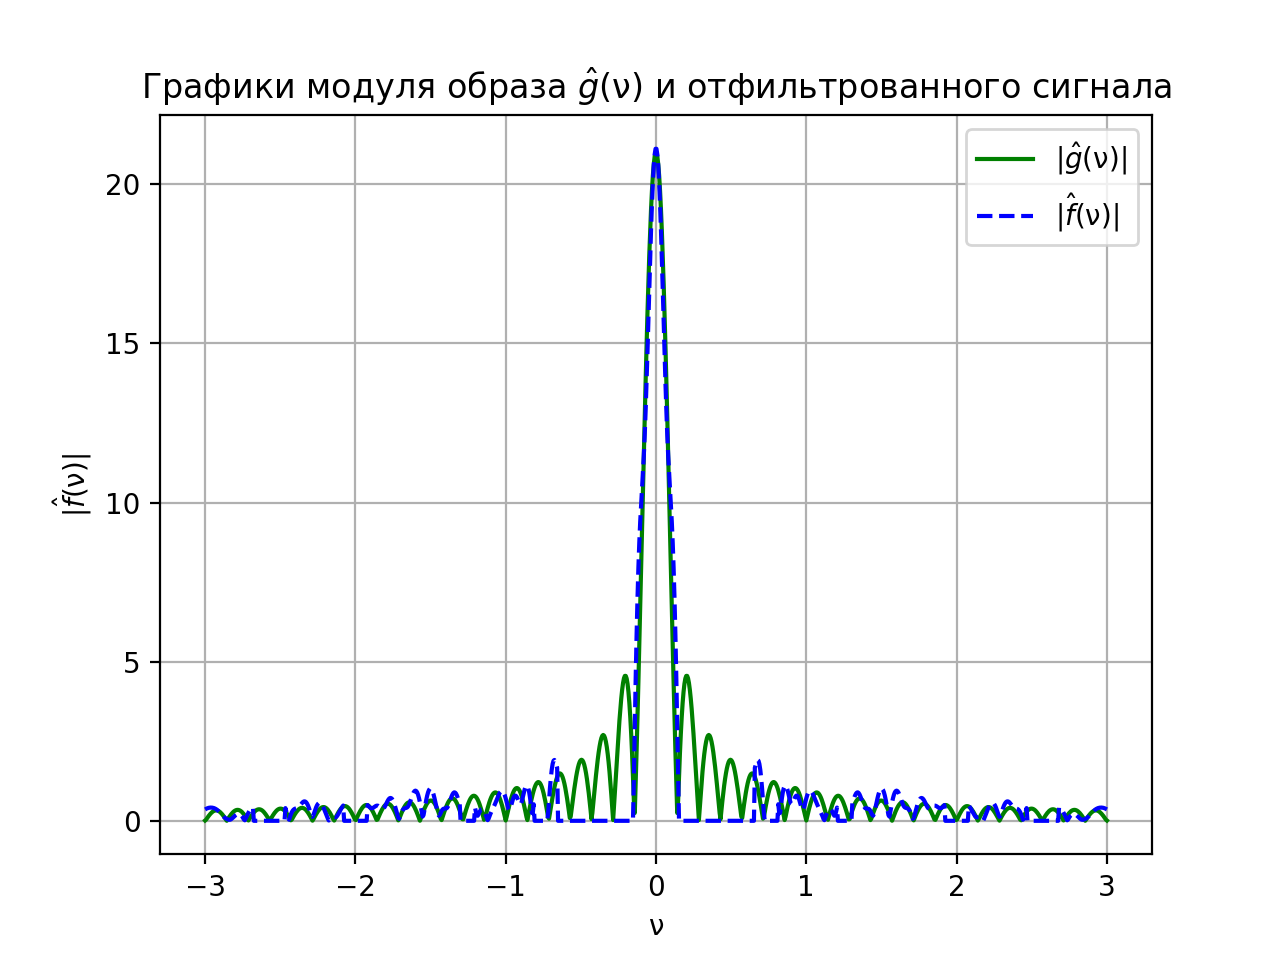
\includegraphics[scale=0.55]{media/1 task/specific_freq/Fourier_Image_Comparison_2_4_2_-0,65:-0,153_-0,8044:-0,72_-1,3:-1,21_-2,07:-1,922_-2,67:-2,47.png}
    \caption{Сравнительные графики модулей Фурье-образа $g(t)$ и отфильтрованного сигнала при $b=2$,  $c=4$,  $d=2$}
    \label{fig:fourc_2_4_2_5intervlas}
\end{figure}

\clearpage

\begin{figure}[ht!]
    \centering
    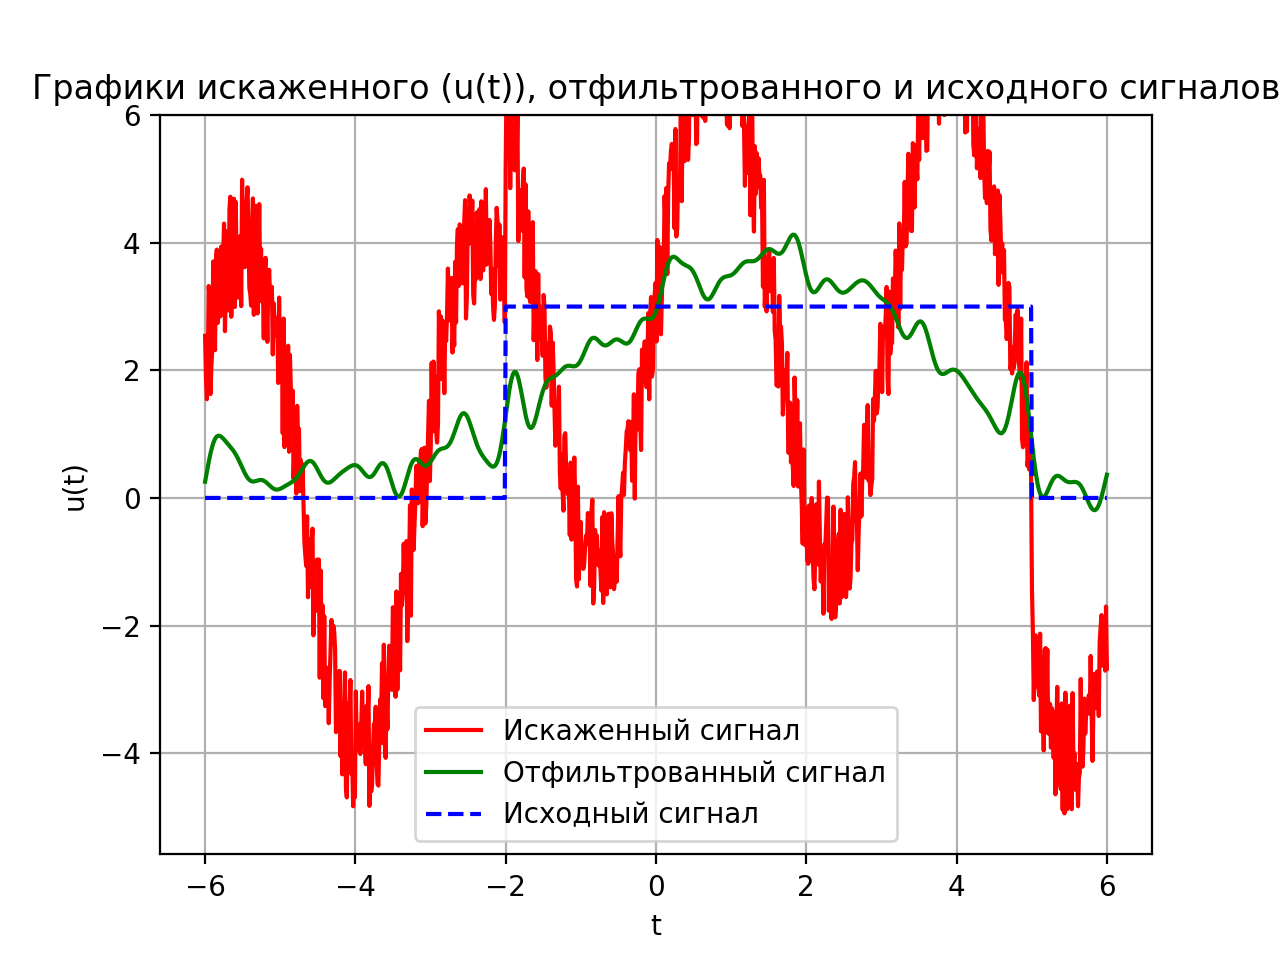
\includegraphics[scale=0.65]{media/1 task/specific_freq/Cleaned_2_4_2_-0,65:-0,153_-0,8044:-0,72_-1,3:-1,21_-2,07:-1,922_-2,67:-2,47.png}
    \caption{Графики  $u(t)$, отфильтрованного и исходного сигналов при $b=2$,  $c=4$,  $d=2$}
    \label{fig:cleaned_2_4_2_5intervals}
\end{figure}


К сожалению, с помощью жёсткой фильтрации нам не удалось добиться того, чтобы отфильтрованный сигнал был бы идентичен или близок к исходному сигналу. Перебрав множество комбинаций интервалов, было решено остановится на интервалах, изображенных на рисунках \ref{fig:cleaned_2_4_2}, \ref{fig:cleaned_2_4_2_2intervals} и \ref{fig:cleaned_2_4_2_5intervals}, так как при них мы смогли добиться наилучших результатов. Стоит отметить, что наиболее сглаженный сигнал был получен при фильтрации 5 интервалов. Однако мы не можем выделить наиболее близкий к исходному сигнал, потому что во всех 3 случаях мы получили очень похожие между собой сигналы, которые могут отличаться значениями в некоторые моменты времени.

Жёсткая фильтрация не может эффективно сглаживать искажения, которые одновременно вызваны синусоидальным и хаотическим шумами. Подобная комбинация искажает Фурье-образ таким образом, что его фильтрация только методом исключения определённых диапазонов частот не позволяет качественно избавиться от помех. Исключение широкого диапазона частот приводит к тому, что мы теряем частоты, которые играли важную роль в оригинальном сигнале. В итоге мы получаем сигнал, имеющий черты исходного, но не являющейся результатом, который можно назвать удовлетворительным.
\clearpage

\subsection{Низкие частоты}

Возьмём сигнал с параметрами $b=4$ $c=2$ $d=2$, график которого приведён ниже:

\begin{figure}[ht!]
    \centering
    \includegraphics[scale=0.5]{media/1 task/low_freq/Noisy_4_2_2.png}
    \caption{График $u(t)$ при $b=4$, $c=2$ и $d=2$}
    \label{fig:noisy_4_2_2}
\end{figure}

\subsubsection{Частоты, частоты и ещё раз частоты!}

В качестве частоты среза будут выступать значения $0.4, 0.6, 1.2, 1.8$ Гц. Графики приведены ниже:

\begin{figure}[ht!]
    \centering
    \includegraphics[scale=0.5]{media/1 task/low_freq/Fourier_Image_4_2_2_-0,4.png}
    \caption{Графики модулей Фурье-образа $u(t)$ и отфильтрованного сигнала при $\nu_0=0.4$ Гц}
    \label{fig:four_4_2_2_0.4}
\end{figure}

\begin{figure}[ht!]
    \centering
    \includegraphics[scale=0.55]{media/1 task/low_freq/Fourier_Image_Comparison_4_2_2_-0,4.png}
    \caption{Сравнительные графики модулей Фурье-образа $g(t)$ и отфильтрованного сигнала при $\nu_0=0.4$ Гц}
    \label{fig:fourc_4_2_2_0.4}
\end{figure}

\begin{figure}[ht!]
    \centering
    \includegraphics[scale=0.55]{media/1 task/low_freq/Fourier_Image_4_2_2-0,5975975975975976.png}
    \caption{Графики модулей Фурье-образа $u(t)$ и отфильтрованного сигнала при $\nu_0=0.6$ Гц}
    \label{fig:four_4_2_2_0.6}
\end{figure}

\begin{figure}[ht!]
    \centering
    \includegraphics[scale=0.55]{media/1 task/low_freq/Fourier_Image_Comparison_4_2_2-0,5975975975975976.png}
    \caption{Сравнительные графики модулей Фурье-образа $g(t)$ и отфильтрованного сигнала при $\nu_0=0.6$ Гц}
    \label{fig:fourc_4_2_2_0.6}
\end{figure}

\begin{figure}[ht!]
    \centering
    \includegraphics[scale=0.55]{media/1 task/low_freq/Fourier_Image_4_2_2-1,1981981981981982.png}
    \caption{Графики модулей Фурье-образа $u(t)$ и отфильтрованного сигнала при $\nu_0=1.2$ Гц}
    \label{fig:four_4_2_2_1.2}
\end{figure}

\begin{figure}[ht!]
    \centering
    \includegraphics[scale=0.55]{media/1 task/low_freq/Fourier_Image_Comparison_4_2_2-1,1981981981981982.png}
    \caption{Сравнительные графики модулей Фурье-образа $g(t)$ и отфильтрованного сигнала при $\nu_0=1.2$ Гц}
    \label{fig:fourc_4_2_2_1.2}
\end{figure}

\begin{figure}[ht!]
    \centering
    \includegraphics[scale=0.55]{media/1 task/low_freq/Fourier_Image_4_2_2-1,7987987987987988.png}
    \caption{Графики модулей Фурье-образа $u(t)$ и отфильтрованного сигнала при $\nu_0=1.8$ Гц}
    \label{fig:four_4_2_2_1.8}
\end{figure}

\clearpage

\begin{figure}[ht!]
    \centering
    \includegraphics[scale=0.55]{media/1 task/low_freq/Fourier_Image_Comparison_4_2_2-1,7987987987987988.png}
    \caption{Сравнительные графики модулей Фурье-образа $g(t)$ и отфильтрованного сигнала при $\nu_0=1.8$ Гц}
    \label{fig:fourc_4_2_2_1.8}
\end{figure}


Каждый раз мы берём всё более высокую частоту среза. Посмотрим, как это отразиться на фильтрации:

\begin{figure}[ht!]
    \centering
    \includegraphics[scale=0.75]{media/1 task/low_freq/Cleaned_4_2_2_-0,4.png}
    \caption{Графики  $u(t)$, отфильтрованного и исходного сигналов при $\nu_0=0.4$ Гц}
    \label{fig:cleaned_4_2_2_0.4}
\end{figure}

\clearpage

\begin{figure}[ht!]
    \centering
    \includegraphics[scale=0.75]{media/1 task/low_freq/Cleaned_4_2_2_-0,5975975975975976.png}
    \caption{Графики  $u(t)$, отфильтрованного и исходного сигналов при $\nu_0=0.6$ Гц}
    \label{fig:cleaned_4_2_2_0.6}
\end{figure}

\begin{figure}[ht!]
    \centering
    \includegraphics[scale=0.75]{media/1 task/low_freq/Cleaned_4_2_2_-1,1981981981981982.png}
    \caption{Графики  $u(t)$, отфильтрованного и исходного сигналов при $\nu_0=1.2$ Гц}
    \label{fig:cleaned_4_2_2_1.2}
\end{figure}

\clearpage

\begin{figure}[ht!]
    \centering
    \includegraphics[scale=0.75]{media/1 task/low_freq/Cleaned_4_2_2_-1,7987987987987988.png}
    \caption{Графики  $u(t)$, отфильтрованного и исходного сигналов при $\nu_0=1.8$ Гц}
    \label{fig:cleaned_4_2_2_1.8}
\end{figure}

Во всех случаях у отфильтрованного сигнала отсутствуют характерные для $g(t)$ скачки в точках разрыва. При увеличении частоты разреза $\nu_0$ колебания сигнала становятся похожи на синусоидальные, хаотический шум становится менее заметным, а амплитуда отфильтрованного сигнала становится меньше. 

Это происходит из-за исключения нижних частот, которые играют важную роль в исходном сигнале. При дальнейшем увеличении частоты среза мы оставляем компоненты, вклад которых не столь существенен, поэтому мы получаем графики с увеличенной частотой и уменьшенной амплитудой. 